\documentclass[candidate,subf,href,colorlinks=true
%,fixint=false
%,times
%,facsimile
%,classified
]{disser}

\usepackage[
  a4paper, mag=1000, includefoot,
  left=3cm, right=1cm, top=2cm, bottom=2cm, headsep=1cm, footskip=1cm
]{geometry}
\usepackage[T2A]{fontenc}
\usepackage[utf8]{inputenc}
\usepackage[english,russian]{babel}
\usepackage{graphicx}
\usepackage{amsmath}
\usepackage{comment}
\ifpdf\usepackage{epstopdf}\fi

\usepackage{listings}
\lstloadlanguages{Delphi,C++,Java,HTML,PHP}
\lstset{numbers=left,language=C++,postbreak=\space, breakindent=5pt,breakautoindent
=false,breaklines,tabsize=2,extendedchars=true,escapechar=|,frame=,commentstyle=\itshape,stringstyle=\bfseries}

\usepackage{algpseudocode}
\usepackage{algorithm} 

\usepackage{longtable}
%\usepackage{algorithmicx} 

% Номера страниц сверху и по центру
%\def\headfont{\small}
%\pagestyle{headcenter}
%\chapterpagestyle{empty}
\setcounter{tocdepth}{2}
% Ссылки на работы соискателя включаются в общий список литературы
\let\citemy=\cite

% Использовать полужирное начертание для векторов
\let\vec=\mathbf

% Путь к файлам с иллюстрациями
\graphicspath{{images/}}

\begin{document}
% Включение файла с общим текстом диссертации и автореферата
% (текст титульного листа и характеристика работы).
% Общие поля титульного листа диссертации и автореферата
\institution{\small{МИНИСТЕРСТВО ОБРАЗОВАНИЯ И НАУКИ РОССИЙСКОЙ ФЕДЕРАЦИИ
ФЕДЕРАЛЬНОЕ ГОСУДАРСТВЕННОЕ БЮДЖЕТНОЕ ОБРАЗОВАТЕЛЬНОЕ УЧРЕЖДЕНИЕ ВЫСШЕГО
ПРОФЕССИОНАЛЬНОГО ОБРАЗОВАНИЯ <<ГОСУДАРСТВЕННЫЙ
УНИВЕРСИТЕТ --- УЧЕБНО-НАУЧНО-ПРОИЗВОДСТВЕННЫЙ КОМПЛЕКС>>}}

\topic{Разработка подсистемы аутентификации пользователей в сети корпоративных
информационных порталов с применением портативного цифрового ключа доступа}

\author{Силаев Павел Павлович}

\specnum{080800.68}
\spec{Системы корпоративного управления}
%\specsndnum{01.04.07}
%\specsnd{Физика конденсированного состояния}

\sa{Лазарев Сергей Александрович}
\sastatus{к.~э.~н., доцент.}
%\sasnd{ФИО второго руководителя}
%\sasndstatus{к.~ф.-м.~н., проф.}

%\scon{ФИО консультанта}
%\sconstatus{д.~ф.-м.~н., проф.}

\city{Орел}
\date{\number\year}

% Общие разделы автореферата и диссертации
\mkcommonsect{actuality}{Актуальность работы.}{%
В современном мире к корпоративным
информационным системам (далее КИС) предъявляют высочайшие требования. В первую
очередь это касается функциональных требований и, как следствие, требований безопасности.
Одним из важнейших элементов КИС является доступ к корпоративным
информационным порталам, к которым всегда предъявлялись особые требования по
обеспечению безопасности.

С развитием информационных технологий резко возросло количество
несанкционированных проникновений. Это затрагивает вопрос о разработке
единого, универсального и высокозащищенного механизма доступа к
web-порталам, что, в свою очередь, позволит развивать корпоративные
информационные системы, системы электронного документооборота, а так же
способствует созданию информационных ассоциаций.~\cite{accociate}
Поэтому решение данной проблемы является сейчас одной из самых актуальных
задач.}

\mkcommonsect{object}{Объектом исследования}{%
является совокупность методик, моделей, алгоритмов и аппаратных средств
распределённой системы доступа к сети корпоративных порталов.}

\mkcommonsect{subject}{Предметом исследования}{% выступают процессы
осуществления доступа к порталам по средствам распределённой системы с помощью
портативных носителей идентификационной информации.}

\mkcommonsect{objective}{Цель диссертационной работы}{%
состоит в разработке подсистемы аутентификации
пользователей в сети корпоративных
информационных порталов с применением
портативного цифрового ключа доступа

Для достижения поставленной цели были решены следующие задачи:
\begin{enumerate}
  \item Анализ способов доступа к сети корпоративных порталов;
  \item Создание формализованных
методов и моделей функционирования системы доступа к сети корпоративных
информационных порталов;
\item Формирование технологических и алгоритмических решений
по построению системы доступа к корпоративным информационным порталам;
\item Реализация
программно-аппаратного средства доступа к сети корпоративных порталов с помощью
портативного цифрового ключа доступа.
\end{enumerate}
}

\mkcommonsect{novelty}{Научная новизна}{%
исследования заключается в разрабатываемых:
\begin{itemize}
  \item технологии доступа к сети порталов; 
  \item модели функционирования сети корпоративных информационных  порталов.
\end{itemize} 
}

\mkcommonsect{value}{Практическая значимость}{%
Результаты, изложенные в диссертации, могут быть использованы совместно с
распределенной системой управления доступом для сети
порталов.~\cite{conf_itnop_lsa_concept}}

\mkcommonsect{results}{%
На защиту выносятся следующие основные результаты и положения:}{%
Текст о результатах.
}

\mkcommonsect{approbation}{Апробация работы}{%
Основные результаты диссертации докладывались на следующих конференциях: 
}

\mkcommonsect{pub}{Публикации.}{%
Материалы диссертации опубликованы в $5$ печатных работах, из них $2$
статьи в рецензируемых журналах вхожящих в перечень ВАК, $2$ статьи в
сборниках трудов конференций.
}

\mkcommonsect{contrib}{Личный вклад автора}{% 
Содержание диссертации и основные
положения, выносимые на защиту, отражают персональный вклад автора в
опубликованные работы.
Подготовка к публикации полученных результатов проводилась совместно с
соавторами, причем вклад диссертанта был определяющим. Все представленные в
диссертации результаты получены лично автором.
}

\mkcommonsect{struct}{Структура и объем диссертации}{%
Диссертация состоит из введения,  $4ех$ глав, заключения и библиографии.
Общий объем диссертации $p_1$ страниц, из них $p_2$ страницы текста, включая $p_3$ рисунков.
Библиография включает $b_1$ наименований на $p_4$ страницах.
}

% номер копии для грифа секретности
%\copynum{1}
% класс доступа
%\classlabel{Для служебного пользования}

\title{МАГИСТЕРСКАЯ ДИССЕРТАЦИЯ\\}

\maketitle

%%
%% Titlepage in English
%%
%
%\institution{Name of Organization}
%
%\title{PhD Thesis}
%
%% Topic
%\topic{Dummy Title}
%
%% Author
%\author{Author's Name}
%
%\specnum{01.04.05}
%\spec{Optics}
%
%%\specsndnum{01.04.07}
%%\specsnd{Condensed matter physics}
%
%\sa{I.\,I.~Ivanov}
%\sastatus{Professor}
%%\sasnd{P.\,P.~Petrov}
%%\sasndstatus{Professor}
%
%% Scientific consultant
%%\scon{B.\,B.~Baranov}
%%\sconstatus{Professor}
%
%% City & Year
%\city{Saint Petersburg}
%\date{\number\year}
%
%\maketitle[en]

\tableofcontents

\intro

Каждый пользователь глобальной сети «Интернет» ежедневно сталкивается с
необходимостью входа на какой-либо ресурс, зарегистрировав себя в системе. Этот
процесс необходим для:
\begin{itemize}
  \item обеспечения конфиденциальности важных данных пользователя, который
  хранит их на данном ресурсе;
\item разграничения прав доступа к этому ресурсу.
\end{itemize}

Процесс регистрации пользователя в системе состоит из трех взаимосвязанных,
выполняемых последовательно процедур: идентификации, аутентификации и
авторизации.

Идентификация --- это процедура распознавания субъекта по его идентификатору. В
процессе регистрации субъект предъявляет системе свой идентификатор и она
проверяет его наличие в своей базе данных. Субъекты с известными системе
идентификаторами считаются легальными (законными), остальные субъекты относятся
к нелегальным.

Аутентификация --- процедура проверки подлинности субъекта, позволяющая
достоверно убедиться в том, что субъект, предъявивший свой идентификатор, на
самом деле является именно тем субъектом, идентификатор которого он использует.
Для этого он должен подтвердить факт обладания некоторой информацией, которая
может быть доступна только ему одному (пароль, ключ и т.п.).

Авторизация --- процедура предоставления субъекту определенных прав доступа к
ресурсам системы после прохождения им процедуры аутентификации. Для каждого
субъекта в системе определяется набор прав, которые он может использовать при
обращении к ее ресурсам.

Для того чтобы обеспечить управление и контроль над данными процедурами,
дополнительно используются процессы администрирования и аудита.

Администрирование --- процесс управления доступом субъектов к ресурсам системы.
Данный процесс включает в себя:
\begin{itemize}
  \item создание идентификатора субъекта (создание учетной записи пользователя) в
системе;
\item управление данными субъекта, используемыми для его аутентификации
(смена пароля, издание сертификата и т.п.);
\item управление правами доступа
субъекта к ресурсам системы.
\end{itemize}

Аудит --- процесс контроля (мониторинга) доступа субъектов к ресурсам системы,
включающий протоколирование действий субъектов при их доступе к ресурсам системы
в целях обеспечения возможности обнаружения несанкционированных действий.
В общем случае, речь идет о пяти основных процедурах процесса
предоставления доступа к информации.

Под системой доступа понимается набор методов и способов, а так же
соответствующий программно-аппаратный комплекс, обеспечивающие процесс
предоставления доступа к конфиденциальной информации.

Идентификационная информация --- набор уникальных параметров, в том числе
секретных, позволяющих пользователю получить доступ к системе.
%
% Используемые далее команды определяются в файле common.tex.
%

% Актуальность работы
\actualitysection
\actualitytext

%Объект исследования
\objectsection
\objecttext

%Предмет исследования
\subjectsection
\subjecttext

% Цель диссертационной работы
\objectivesection
\objectivetext

% Научная новизна
\noveltysection
\noveltytext

% Практическая ценность
\valuesection
\valuetext

% Результаты и положения, выносимые на защиту
\resultssection
\resultstext

% Апробация работы
\approbationsection
\approbationtext

% Публикации
\pubsection
\pubtext

% Личный вклад автора
\contribsection
\contribtext

% Структура и объем диссертации
\structsection
\structtext
%\review

\chapter{Анализ существующих систем доступа к информационным порталам}

\section{Корпоративные порталы}

Понятие корпоративного информационного портала (Enterprise Information Portal --
EIP) было введено компанией Merrill Lynch в ноябре 1998 года. Вслед за этим
последовало определение и многих других типов порталов.
Существует много самых разных определений корпоративным порталам, приведем
только исторически первое определение компании Merrill Lynch: <<Корпоративные
информационные порталы -- это приложения, которые позволяют компаниям раскрывать
информацию, хранящуюся внутри и вне организации, и предоставлять пользователям
единый шлюз доступа к персонализированной информации, необходимой для принятия
бизнес-решений>>. Они являются <<…совокупностью программных приложений, которые
консолидируют, управляют, анализируют и распространяют информацию по всему
предприятию и за его пределами>>~\cite{kis_eip}.

Определение корпоративного портала должно исходить из той цели, которую компания
ставит (или может ставить, но еще не знает об этом) перед корпоративным
порталом. В этом смысле у каждой компании будет свое определение, но именно того
корпоративного портала, который ей и требуется.

Если отойти от существующих определений и от вопроса возможностей корпоративного
портала, то для территориально разделенной компании имеющей корпоративную
информационную систему (КИС) в центральном офисе, можно сформулировать следующие
цели создаваемого корпоративного портала:
\begin{enumerate}
  \item Обеспечить всем работникам компании независимо от их территориального
нахождения доступ к КИС компании (естественно, в соответствии с полномочиями
разграничения доступа), доступ и к требуемой информации, и к требуемым
приложениям, необходимым для плодотворной работы. Т. е. при такой постановке
корпоративных информационных порталов (далее КИП) -- это средство обеспечения
прозрачного доступа к центральной КИС для всех сотрудников;
\item Обеспечить доступ к КИС компании партнерам и клиентам компании (естественно,
в соответствии с самыми строгими полномочиями разграничения доступа), доступ и к
требуемой информации, и к требуемым приложениям, необходимым для получения
информации, осуществления заказа и т.д.
\end{enumerate}

При этом корпоративный портал, фактически, является веб-интерфейсом КИС. Многие
производители КИС класса ERP включают в свои системы корпоративные порталы и
веб-интерфейсы (Oracle, Baan, Парус), а совсем недавно появились КИС класса
ERP II, основные отличия которых от ERP-КИС следующие:
\begin{enumerate}
  \item Выход КИС за пределы компании, <<прозрачное>> взаимодействие компании с
контрагентами (заказчиками, поставщиками, банками, налоговыми органами и др.).
Открытие максимального числа информационных процессов, развитие так называемой
<<коллаборативной коммерции>> (c-commerce) -- совместного электронного бизнеса
предприятия, деловых партнеров и потребителей;
\item Максимально полный охват всех бизнес-процессов компании.
\end{enumerate}

Таким образом, понятия корпоративной информационной системы и корпоративного
портала начинают сливаться. Поэтому можно сформулировать наиболее полное
определение корпоративных информационных порталов.

Корпоративные информационные порталы --- это web-сайты, которые позволяют
компании раскрывать информацию, хранящуюся внутри и вне организации, и предоставить
каждому пользователю единую точку доступа к предназначенной для него информации,
необходимой для принятия обоснованных управленческих решений.~\cite{opred_kis}

Исходя из функциональных особенностей сети корпоративных порталов, одну из
основополагающих ролей играет система аутентификации пользователей и
разграничение прав доступа.

Для определения принадлежности пользователя к сети корпоративных порталов
необходимо осуществить эффективный алгоритм аутентификации. Основные методы
аутентификации пользователей различаются, прежде всего, аутентификациионными
факторами. Аутентификационный фактор --- определенный вид информации,
предоставляемый субъектом системе при его аутентификации -- нечто, нам
известное: пароль. Отличительная характеристика представляет собой секретную
информацию, которая неизвестна непосвященным людям. При некомпьютерном использовании это
может быть произносимый голосом пароль или запоминаемая комбинация для замка. В
случае вычислительных систем это может быть пароль, вводимый с помощью
клавиатуры. Разработчики могут дешево и легко реализовать паролевый механизм.
Запоминаемое секретное слово может быть наиболее удобным средством с точки
зрения перемещающихся пользователей, т.е. для людей, которые подключаются к
системе из непредсказуемых удаленных мест. Однако использование паролей не
лишено недостатков. Во-первых, их эффективность зависит от секретности, а
хранить пароли в тайне нелегко. Существует бессчетное количество способов
выведать или перехватить пароль, и обычно обнаружить активную разведку до
нанесения урона невозможно. Во-вторых, развитие методов нападения сделало для
взломщиков определение паролей, обычно выбираемых людьми, относительно простым
делом. Даже если выбираются трудно угадываемые пароли, их где-нибудь записывают,
чтобы при необходимости иметь под рукой. Но, конечно же, записываемый пароль
более уязвим в плане возможной кражи, чем запоминаемый. Даже действующие из
лучших побуждений люди в какой-то момент нарушают правила использования паролей
просто для того, чтобы иметь возможность воспользоваться своим компьютером
именно тогда, когда в этом возникнет необходимость. Нечто, присущее нам:
биометрика. Отличительной характеристикой является какая-нибудь физическая
особенность, уникальная для аутентифицируемого лица. До появления компьютеров
это могли быть личная подпись, фотография, отпечаток пальца или письменное
описание внешнего вида человека.~\cite{auth_n_aut}

При компьютерном использовании отличительная характеристика физического лица
измеряется и сравнивается с ранее полученными данными, снятыми с достоверно
установленной личности. В хорошо известных методиках для аутентификации
используются голос человека, отпечатки пальцев, письменная подпись, форма кисти
или особенности радужной оболочки глаза. Нечто, имеющееся у нас: устройство
аутентификации. Отличительной характеристикой является наличие у авторизованного
лица некоего конкретного предмета. При некомпьютерном использовании это могли
быть печать или ключ от замка. В компьютерных системах это может быть не более
чем носитель с файлом данных, содержащим отличительную характеристику. Часто
характеристика встраивается в устройство, например в карту с магнитной полосой,
смарт-карту, USB ключ или в OTP токен. Кроме того, подобные устройства часто
предлагают возможность так называемой многофакторной аутентификации.
Многофакторная аутентификация — аутентификация, в процессе которой используются
аутентификационные факторы нескольких типов. Например, пользователь должен
предоставить смарт-карту и дополнительно ввести пароль. Также используются
понятия двухфакторной и трехфакторной аутентификации при использовании в
процессе аутентификации комбинации двух и трех типов аутентификационных факторов
соответственно.

Метод аутентификации (метод регистрации) --- специфика использования
определенного типа аутентификационных факторов в процедуре аутентификации. Кроме
методов локальной аутентификации -- входа пользователя локально в компьютер,
существуют методы для аутентификации в локальных вычислительных сетях, при
доступе к удаленным ресурсам, веб приложениям и др.

Немаловажной составляющей корпоративных информационных порталов является
электронный документооборот. Документооборот --- движение документов в
организации с момента их создания или получения до завершения исполнения или
отправления.~\cite{GOST_P51141}

Комплекс работ с документами: прием, регистрация, рассылка, контроль исполнения,
формирование дел, хранение и повторное использование документации, справочная
работа.

Электронный документооборот (ЭДО) представляет собой единый механизм по работе с
документами, представленными в электронном виде, с реализацией концепции
<<безбумажного делопроизводства>>.

Необходимость в автоматизации управления документооборотом обусловлено
повышением эффективности организационно-распорядительного документооборота и
работы функциональных специалистов, создающих документы и использующих их в
повседневной работе.

Достоинства электронного документооборота:
\begin{enumerate}
  \item многокритериальный поиск документов;
  \item контроль исполнения документов;
  \item регистрация документов;
  \item ввод резолюций к документам;
  \item распределенная
обработка документов в сети;
  \item  распределение прав доступа к различным
документам и функциям системы;
  \item ведение нескольких картотек документов;
  \item работа с проектами документов;
  \item распределение находящихся на исполнении
документов по <<папкам>> в зависимости от стадии исполнения документа:
поступившие, на исполнении, на контроле и другие;
  \item формирование стандартных
отчетов;
  \item обмен документами по электронной почте;
  \item списание документов в дело;
  \item отслеживание перемещений бумажных оригиналов и копий документов,
ведение реестров внутренней передачи документов;
  \item ведение пользовательских
списков должностных лиц, организаций, тематических рубрик, групп документов;
  \item редактирование шаблонов выходных печатных форм.~\cite{kuznecov}
\end{enumerate}

Введение электронного документооборота позволяет снизить количество служб,
занятых работой с документами (курьеров, канцелярских работников и т. п.).
Для обеспечения электронного документооборота необходимо использование
подсистемы управления обменом электронно-цифровой подписи.

Электронно-цифровая подпись --- атрибут электронного документа, используемый для
защиты информации от несанкционированного использования и подделки.

Электронно-цифровая подпись формируется путем криптографического преобразования
информации с закрытым ключом, что позволяет определить владельца сертификата
ключа подписи и обеспечить неотказуемость подписавшегося от документа, а также
проверить полученную информацию на отсутствие ошибок и неточностей. Электронный
документ --- это документ, подготовленный с использованием системы электронного
документооборота (далее СЭД), зафиксированный на материальном носителе в виде
объекта СЭД и снабженный реквизитами, с помощью которых можно идентифицировать место, время
создания и автора документа.

 Чаще всего цифровые подписи используются для подтверждения имени отправителя,
 основываясь на том, что лишь он один владеет уникальным закрытым ключом,
 которому соответствует полученный открытый ключ. Также электронная подпись
 иногда используется для датирования документа с помощью штампа времени:
 доверенная сторона подписывает документ штампом времени с помощью своего
 специального закрытого ключа, подтверждая существование документа в данный
 момент, обозначенный в цифровой подписи.
 
В случае если электронно-цифровая подпись ставится для удостоверения личности
отправителя: сторона, которой доверяют априори, предоставляет открытый ключ и
информацию о владельце закрытого ключа получателю документа -- получается
иерархия доверия.

\section{Анализ технологических решений по осуществлению аутентификации}

Для осуществления аутентификации существует множество технологических решений.
Рассмотрев все возможные технические и программные аспекты, можно будет сделать
вывод относительно принятия решения о применении наиболее эффективного
алгоритма.

\subsection{Биометрический метод}

Современные технологии способны обеспечить удостоверение личности человека,
используя характерные только для него одного характеристики. Данные технологии
основаны на практическом применении знаний научной дисциплины биометрии. Данная
дисциплина занимается статистическим анализом биологических наблюдений и
явлений. Биометрическая характеристика --- это измеримая физиологическая или
поведенческая черта живого человека. Некоторые биометрические характеристики
уникальны для данного человека, и их можно использовать для установления
личности или проверки декларируемых личных данных:
\begin{itemize}
  \item для идентификации пользователя (вместо ввода имени пользователя);
  \item для однофакторной аутентификации пользователя;
  \item совместно с паролем или
аутентификационным токеном(таким, как смарт-карта);
  \item для обеспечения
двухфакторной аутентификации.
\end{itemize}

Биометрические характеристики делятся на группы. Физиологические биометрические
характеристики (также называемые физическими биометрическими характеристиками,
статическими биометрическими характеристиками) --- биометрические
характеристики, основанные на данных, полученных путем измерения анатомических
характеристик человека, таких, как отпечаток пальца, форма лица или кисти,
сетчатка глаза.

Поведенческие биометрические характеристики (также называемые динамическими
биометрическими характеристиками) -- биометрические характеристики, основанные
на данных, полученных путем измерения действий человека.
Характерной чертой для поведенческих характеристик является их протяженность во
времени -- измеряемое действие имеет начало, середину и конец. К примеру: голос,
подпись. Хотя биометрические технологии отличаются в объектах и способах
измерений, все биометрические системы работают одинаково. Пользователь
предоставляет образец (sample) -- опознаваемое необработанное изображение или
запись физиологической или поведенческой характеристики посредством
регистрирующего устройства (например, сканера или камеры). Этот биометрический
образец обрабатывается для получения информации об отличительных признаках, в
результате чего получается контрольный шаблон (или шаблон для проверки). Шаблоны
представляют собой числовые последовательности. Сам образец невозможно
восстановить из шаблона. Результат проверки других аутентификационных данных,
как правило, однозначен --- это решение «да» или «нет» (пароль совпал или нет).

В случае проверки контрольного шаблона результат иной. Контрольный шаблон
сравнивается с эталонным шаблоном (или зарегистрированным шаблоном), созданным
на основе нескольких образцов, определенной физиологической или поведенческой
характеристики пользователя, взятых при его регистрации в биометрической
системе. Поскольку эти два параметра (контрольный и эталонный шаблон) полностью
никогда не совпадают, то степень совпадения должна превышать определенную
настраиваемую пороговую величину. Соответственно в биометрических системах
контрольный шаблон может быть ошибочно признан:
\begin{itemize}
  \item соответствующим эталонному шаблону другого лица;
  \item не соответствующим эталонному шаблону данного
пользователя, несмотря на то, что этот пользователь зарегистрирован в
биометрической системе.
\end{itemize}

Точность биометрической системы измеряется двумя
параметрами:

\begin{itemize}
  \item коэффициентом неверных совпадений (FMR), также известным под названием «ошибка
типа I» или «вероятность ложного допуска» (FAR);
  \item коэффициентом неверных
несовпадений (FNMR), также известным под названием «ошибка типа II» или
«вероятность ложного отказа в доступе» (FRR).
\end{itemize}~\cite{auth_n_aut} 

Биометрическая аутентификация обычно является одним из наиболее легких подходов
для тех людей, которые должны проходить аутентификацию. В большинстве случаев
хорошо спроектированная биометрическая система просто снимает показания с
человека и правильно выполняет аутентификацию. Однако все преимущества сводятся
на нет несколькими недостатками. Как правило, по сравнению с другими системами,
приобретение, установка и эксплуатация оборудования стоят дорого. При
дистанционном использовании биометрические показания подвержены риску перехвата:
похититель может воспроизвести запись показаний, чтобы замаскировать себя под
владельца, или использовать их в целях выслеживания последнего. Если
биометрические показатели попадают в плохие руки, то их владелец не имеет
способа восполнения ущерба, так как биометрические особенности невозможно
изменить. Кроме того, сам процесс аутентификации сложен. Сложно также сделать
систему достаточно чувствительной, чтобы она отвергала посторонних пользователей
и при этом время от времени не отвергала своих. Биометрические показатели также
могут быть признаны негодными вследствие физиологических изменений и телесных
повреждений. Был случай, когда биометрическое устройство не впустило в режимное
помещение работавшую там женщину, потому что из-за беременности у нее изменилась
картина кровеносных сосудов в сетчатке глаз. Несмотря на то, что криптография с
открытым ключом может обеспечивать аутентификацию пользователя, сам по себе
закрытый ключ подобен паспорту без фотографии. Закрытый ключ, хранящийся на
жестком диске компьютера владельца, уязвим по отношению к прямым и сетевым
атакам. Достаточно подготовленный злоумышленник может похитить персональный ключ
пользователя и с помощью этого ключа представляться этим пользователем. Защита
ключа с помощью пароля помогает, но недостаточно эффективно -- пароли уязвимы по
отношению ко многим атакам. Несомненно, требуется более безопасное хранилище.

\subsection{Смарт-карты}

Смарт-карты --- пластиковые карты стандартного размера банковской карты
(стандарт ISO 7816 1), имеющие встроенную микросхему. Они находят все более широкое
применение в различных областях, от систем накопительных скидок до кредитных и
дебетовых карт, студенческих билетов и телефонов стандарта GSM. Для
использования смарт-карт в компьютерных системах необходимо устройство чтения
смарт-карт. Несмотря на название -- устройство чтения (или считыватель),
большинство подобных оконечных устройств, или устройств сопряжения (IFD),
способны как считывать, так и записывать информацию, если позволяют возможности
смарт-карты и права доступа. Устройства чтения смарт-карт могут подключаться к
компьютеру посредством последовательного порта, слота PCMCIA или USB. Устройство
чтения смарт-карт также может быть встроено в клавиатуру. Как правило, для
доступа к защищенной информации, хранящейся в памяти смарт-карты, требуется
пароль, называемый PIN кодом (англ. Personal Identification Number --
персональный идентификационный номер).~\cite{thesis_smart_card}

\subsection{Аппаратный генератор одноразовых паролей}

В основе всех методов аутентификации с использованием пароля лежит предположение
о том, что только законный пользователь может успешно пройти проверку личности,
что только он знает свой пароль. Часто злоумышленник может легко узнать
идентификатор пользователя. Особенно если в качестве идентификатора пользователя
используется не случайная строка символов, состоящая из букв и цифр, а «имя
пользователя». Так как обычно <<имя пользователя>> -- это различные варианты
комбинации имени и фамилии пользователя, то определить имя пользователя не
составляет большого труда. Соответственно, если злоумышленнику удастся узнать
еще и пароль, то злоумышленнику будет легко представиться соответствующим
пользователем. Сколь бы ни был пароль засекречен, узнать его иногда не слишком
трудно. Злоумышленник может сделать это, используя различные способы атак. Для
каждой из этих атак есть методы защиты. Но большинство из этих методов обладают
различными недостатками. Некоторые виды защиты достаточно дороги (борьба с
паразитным излучением оборудования), другие создают неудобства для пользователей
(правила формирования пароля, использование длинных паролей).

Один из вариантов защиты от различных атак на аутентификацию по паролю -- это
переход на аутентификацию с использованием одноразовых паролей.

Одноразовые пароли (One Time Passwords -- OTP) -- динамическая
аутентификационная информация, генерируемая для единичного использования с помощью
аутентификационных токенов (программных или аппаратных).
OTP токен -- мобильное персональное устройство, принадлежащее определенному
пользователю, генерирующее одноразовые пароли, используемые для аутентификации
данного пользователя. Аутентификация с одноразовым паролем обладает
устойчивостью к атаке анализа сетевых пакетов, что дает ей значительное
преимущество перед запоминаемыми паролями. Несмотря на то, что злоумышленник
может перехватить пароль методом анализа сетевого трафика, поскольку пароль
действителен лишь один раз или в течение ограниченного промежутка времени, у
злоумышленника, в лучшем случае, есть весьма ограниченная возможность
представиться пользователем посредством перехваченной информации. Для того чтобы
сгенерировать OTP, необходимо иметь OTPтокен. Таким образом, при использовании
OTP вместо аутентификационного фактора <<нечто, нам известное>>, применяется
другой аутентификационный фактор -- <<нечто, имеющееся у нас>>.

Другим важным преимуществом аутентификационных устройств является то, что многие
из них требуют от пользователя введения PIN кода или пароля, который может
использоваться различными способами, в частности:
\begin{itemize}
  \item для активации OTP токена;
  \item в качестве дополнительной информации, используемой
при генерации OTP;
  \item для предъявления серверу аутентификации вместе с OTP.
\end{itemize}

В этих методах аутентификации используются два аутентификационных фактора.
Поэтому они относятся к двухфакторной аутентификации. OTP токены имеют небольшой
размер и выпускаются в виде(форм факторы):
\begin{itemize}
  \item карманного калькулятора;
  \item брелока;
  \item смарт карты;
  \item устройства,
комбинированного с USB ключом;
  \item специального программного обеспечения для
карманных компьютеров.
\end{itemize}

В качестве примера решений OTP можно привести линейкуRSA
SecurID, ActivCard Token, комбинированный USB ключAladdin eToken NG OTP.
~\cite{auth_n_aut}

\subsection{USB ключи}

Некоторые производители выпускают другие виды аппаратных устройств,
представляющие собой комбинацию смарт карты и устройства чтения смарт карт. Они
по свойствам памяти и вычислительным возможностям полностью аналогичны смарт
картам. Наиболее популярны аппаратные «ключи», использующие порт USB. USB ключи
привлекательны для некоторых организаций, поскольку USB стал стандартным портом
для подключения периферийных устройств: организации не нужно приобретать для
пользователей какие бы то ни было считыватели. Аутентификацию на основе смарт
карт и USB ключей сложнее всего обойти, так как используется уникальный
физический объект, которым должен обладать человек, чтобы войти в систему. В
отличие от паролей владелец быстро узнает о краже и может сразу принять
необходимые меры для предотвращения ее негативных последствий. Кроме того,
реализуется двухфакторная (а в случае решений совместно с биометрической
информацией и трехфакторная) аутентификация. Основными слабыми местами являются
более высокая стоимость реализации и риск дополнительных расходов, связанных с
потерей аппаратуры. Смарт карты, USB ключи и другие устройства аутентификации
могут повысить надежность служб PKI: смарт карта может использоваться для
безопасного хранения закрытых ключей пользователя, а также для безопасного
выполнения криптографических преобразований. Безусловно, устройства
аутентификации не обеспечивают абсолютную безопасность, но надежность их защиты
намного превосходит возможности обычного настольного компьютера. Хранить и
использовать закрытый ключ можно по-разному, и разные разработчики используют
различные подходы.

Наиболее простой из них -- использование устройства аутентификации в качестве
защищенного носителя аутентификационной информации: при необходимости карта
экспортирует закрытый ключ, и криптографические операции осуществляются на
рабочей станции. Этот подход является не самым совершенным с точки зрения
безопасности, зато относительно легко реализуемым и предъявляющим невысокие
требования к устройству аутентификации. В качестве примера подобного рода
устройств аутентификации можно привести Aladdin eToken R2, Rainbow iKey 1000,
Актив ruToken. Два следующих подхода более безопасны, поскольку предполагают
выполнение устройством аутентификации криптографических операций. В первом
случае пользователь генерирует ключи на рабочей станции и сохраняет их в памяти
устройства, во втором — с помощью устройства. В обоих случаях, после того как
закрытый ключ сохранен, его нельзя извлечь из устройства и получить любым другим
способом. Генерация ключевой пары вне устройства. В этом случае пользователь
может сделать резервную копию закрытого ключа. Если устройство выйдет из строя,
будет потеряно, повреждено или уничтожено, пользователь сможет сохранить тот же
закрытый ключ в памяти нового устройства. Это необходимо, если пользователю
требуется расшифровать какие-либо данные, сообщения и так далее, зашифрованные с
помощью соответствующего открытого ключа. Однако при этом закрытый ключ
пользователя подвергается риску быть похищенным.Генерация ключевой пары с
помощью устройства. В этом случае закрытый ключ не появляется в открытом виде и
нет риска, что злоумышленник украдет его резервную копию. Единственный способ
использования закрытого ключа -- это обладание устройством аутентификации.
Являясь наиболее безопасным, это решение выдвигает высокие требования к
возможностям самого устройства: оно должно обладать функциональностью генерации
ключей и осуществления криптографических преобразований. Это решение также
предполагает, что закрытый ключ не может быть восстановлен в случае выхода
устройства из строя и т.п. Об этом необходимо беспокоиться при использовании
закрытого ключа для шифрования, но не там, где он используется для
аутентификации, или в других службах, использующих цифровые подписи. Подобным
образом способны работать процессорные смарткарты и USB токены на их основе, к
примеру Aladdin eTokenPRO, eToken NG OTP, Rainbow iKey 2000, iKey 3000,
AthenaASECard Crypto, Schlumberger Cryptoflex, ActivCard USB Key и др.~\cite{auth_n_aut}
\section{Рекомендации по применению методов доступа}

При аутентификации с использованием сертификатов открытого ключа должны
использоваться аппаратные устройства аутентификации (смарт карты, USB ключи).
Краеугольным камнем аутентификации с открытым ключом является исключительное
владение пользователя закрытым ключом. Это не может быть обеспечено, если
закрытый ключ хранится или криптографические преобразования осуществляются на
компьютере пользователя.

Халатность пользователей типа 1. Устройства аутентификации могут оставляться на
рабочей станции. Если пользователь, отходя от своего рабочего места, оставляет
смарт карту в устройстве чтения или USB ключ в порту, кто-то другой в офисе
может легко представиться данным пользователем. Защита с помощью PIN кода
эффективна, если сеансы пользователей блокируются после определенного промежутка
бездействия, а для разблокирования необходима повторная аутентификация. Но PIN
коды можно узнавать, например, с помощью «подглядывания из-за плеча».
Организации должны призывать пользователей всегда носить устройства
аутентификации с собой. Это обеспечивается автоматически, если устройства
используются для физического контроля доступа в помещения (к примеру, смарт
карты или USB токены с интегрированными RFID метками)и операционная система
настроена на блокирование пользовательского сеанса при извлечении устройства
аутентификации.

Халатность пользователей типа 2. Устройства аутентификации могут быть утеряны.
Организация, в которой используются устройства аутентификации, будет вынуждена
каждому пользователю, потерявшему свое устройство, выдавать новое временное
устройство или предоставлять временную возможность аутентификации с помощью
альтернативного метода. При этом организация должна следить за тем, чтобы
подобные мероприятия не приводили к существенному ослаблению безопасности. В
качестве мер, уменьшающих риски при потере устройств аутентификации, можно
привести следующие правила издания сертификатов:
\begin{itemize}
  \item использование различных сертификатов (и соответственно ключевых пар) для целей
аутентификации, формирования ЭЦП и шифрования;
  \item использование генерации
ключевой пары вне устройства для сертификатов, предназначенных для шифрования
данных. Такой подход позволит иметь резервные копии ключевой информации на
случай утери устройства. Для архивирования закрытых ключей пользователей
рекомендуется использовать модули аппаратной защиты (HSM);
  \item использование
генерации ключевой пары с помощью устройства аутентификации для создания
сертификата, предназначенного для аутентификации пользователя в системе. Такой
подход позволяет гарантировать уникальность аутентификационных данных (то, что
существует только одно устройство, с помощью которого данный пользователь может
войти в систему, и что нельзя изготовить дубликат аутентификационных данных),
при этом при утере устройства (и последующих отзыве старого
сертификата и издании нового) не происходит потери пользовательской информации.
\end{itemize}

Устройства аутентификации могут быть уязвимы по отношению к логическим и
физическим атакам, а также атакам троянских коней. Каждая организация,
использующая данные устройства в приложениях безопасности, должна быть уверена в
том, что производители устройств и разработчики программного обеспечения
позаботились о принятии соответствующих логических и архитектурных контрмер.
Правда, эти меры могут отрицательно сказаться на удобстве использования
устройств аутентификации.

Логические атаки осуществляются, когда устройство аутентификации работает в
обычных физических условиях, но важная информация получается в результате чтения
трафика, входящего в устройство аутентификации и выходящего из него. Если есть
риск подобных атак, рекомендуется использовать устройства, позволяющие защищать
(к примеру, с помощью потокового шифрования) передаваемую информацию. В
компьютерных системах файлы данных, так или иначе, хранятся в пределах файловой
системы. Доступом к файлам и папкам управляет операционная система, и
рекомендации по назначению прав хорошо известны. Тем не менее список лиц,
которые могут получить доступ к незащищенным конфиденциальным данным,
оказывается весьма обширным. Администратор операционной системы по умолчанию
имеет самый высокий уровень прав доступа. Системный администратор имеет
возможность обратиться по сети к любому диску сервера с помощью так называемых
административных сетевых ресурсов. Не следует забывать и о роли человеческого
фактора. В случае ошибки администратора при настройке прав доступ к
конфиденциальным данным может получить любой пользователь. По оценкам IDC,
примерно 74\% финансовых потерь связаны с проблемами так называемого
«человеческого фактора». Для сравнения: потери от вирусных и хакерских атак
составляют соответственно 4 и 2\%.Также источником угроз являются компьютерные
вирусы, сетевые черви и троянские программы. Если список программного
обеспечения, устанавливаемого на сервере, всегда известен и само программное
обеспечение свободно от вирусов, то компьютеры пользователей могут быть заражены
вирусами и (или) содержать троянские программы. Используя параметры учетной
записи пользователя, работающего в данный момент за зараженным компьютером,
вирус может выполнять сканирование сетевых ресурсов и пытаться прочитать
хранящиеся на них файлы. Если таким пользователем является администратор, то
вирусу становится доступно содержимое дисков сервера через административные
сетевые ресурсы.

В качестве мер для предотвращения подобного рода угроз НСД к данным файловой
системы можно порекомендовать как организационные меры по контролю установленных
прав доступа и аудита их изменения, так и возможность использования
специализированных средств, таких, как программно аппаратные комплексы
криптографической защиты файловой системы с двухфакторной аутентификацией.

Подобные комплексы могут обеспечивать следующие функции:
\begin{itemize}
  \item двухфакторную аутентификацию для доступа к защищенным данным;
  \item защиту данных
на жестких и съемных дисках от несанкционированного доступа методом
«прозрачного» шифрования, в том числе от возможности получения доступа в обход
средств аутентификации и контроля доступа операционной системы с помощью
физического подключения к носителям данных;
  \item контроль сетевого доступа к
защищенным дискам, позволяющий для каждого защищенного диска определить, будет
ли он доступен по сети пользователям или только приложениям, выполняющимся
непосредственно на сервере;
  \item возможность отключения (в том числе с уничтожением
ключевой информации, с помощью которой проводится шифрование) доступа к
защищенной информации в случае возникновения нештатных ситуаций.
\end{itemize}

Примерами такого рода решений могут быть программно аппаратные комплексы для
защиты серверных данных AladdinSecretDisk Server NG, Физтехсофт StrongDisk
Server, ЛАН Крипто Индис Cервер, Control Break SafeBoot Device
Encryption,WinMagic SecureDoc. Доступ к ресурсам информационной системы -- это
фактически доступ к данным, находящимся в хранилище под управлением
СУБД. В таком контексте нарушением безопасности является НСД, который тем или
иным способом может получить потенциальный злоумышленник. Поэтому обеспечение
надежной и безопасной аутентификации — важнейшая задача как для разработчиков,
так и для администраторов систем. Существует несколько основных методов
аутентификации, которые обеспечивают разную степень безопасности. Выбор метода
должен основываться на таких факторах, как:
\begin{itemize}
  \item надежность, достоверность, неотказуемость (неотрицание совершения
  операций);
  \item стоимость решения, стоимость администрирования;
  \item соответствие общепринятым
стандартам;
  \item простота интеграции в готовые решения и новые разработки.
\end{itemize}

Как правило, более надежные методы являются более дорогостоящими как для
разработки, так и для администрирования.
 Наиболее надежным методом аутентификации на сегодняшний день является
 двухфакторная аутентификация с использованием цифровых сертификатов X.509,
 которые хранятся в защищенной памяти смарт карт или USB ключей. Оба этих
 устройства обеспечивают одинаковую степень надежности аутентификации, но смарт
 карты требуют дополнительного оборудования, что, естественно, увеличивает
 стоимость решения. Также необходимо обратить внимание на следующие аспекты:
 \begin{itemize}
   \item интеграцию с внешними системами аутентификации;
   \item безопасность соединений;
   \item защиту данных на любом уровне;
   \item выборочное шифрование данных;
   \item подробный аудит
действий пользователей;
   \item централизованное управление аутентификацией и
авторизацией пользователей.
 \end{itemize}

Обычно разработчики программного обеспечения не
уделяют должного внимания вопросам защиты данных, стараясь по максимуму
удовлетворить пожелания заказчиков по функциональности системы. В результате
подобные проблемы решаются зачастую в процессе внедрения системы, и это приводит
к ситуациям, когда «защищенное» приложение содержит <<секретные>> коды, прошитые
в исходных текстах программ или в файлах настройки. Определенные трудности для
разработчиков представляют ситуации, когда заказчик системы сам толком не
представляет, от кого и что, собственно, следует защищать. Интеграторы при
внедрении систем в организации заказчика уделяют большое внимание защите, но
здесь акценты смещены в сторону внешних атак -- троянов, вирусов, хакеров.
Вопросы <<внутренней>> безопасности и в этом случае остаются открытыми. В такой
ситуации усилия системных администраторов, неосведомленных в полной мере о
бизнес процессах организации, направлены на «урезание» прав пользователей, что
существенно осложняет работу системы в целом, а иногда приводит к ее полной
остановке. Мероприятия по защите информации должны включать решение следующих
вопросов:
\begin{itemize}
  \item определение угроз безопасности и групп потенциальных нарушителей;
  \item определение групп приложений, обеспечивающих бизнес процессы
  организации;
  \item определение категорий данных по уровню доступа;
  \item определение групп
пользователей системы;
  \item определение объектов, хранящих данные и подлежащих
защите;
  \item определение политик безопасности;
  \item определение методов хранения
связей пользователей;
  \item права доступа;
  \item данные;
  \item выбор метода аутентификации и
способов ее реализации;
  \item подготовка методики по обеспечению безопасности
инфраструктуры сети, СУБД, серверов приложений, клиентских приложений.
\end{itemize}

Также весьма популярным способом получения НСД к содержимому базы данных
является попытка прочитать файлы БД на уровне ОС (как обычные файлы). Если
администратором БД не были предприняты дополнительные меры по шифрованию
содержащейся в ней информации (а чаще всего это именно так), то простое
копирование файлов БД по сети и последующий прямой просмотр их содержимого
позволят злоумышленнику получить доступ к хранящейся в БД информации. Довольно
часто IT сотрудники не могут устоять от соблазна <<пронюхать>> информацию,
лежащую на поверхности. И они имеют все возможности для этого, поскольку обладают
привилегиями доступа к файлам. Именно поэтому защищенная система должна быть
спроектирована и построена так, чтобы:
\begin{itemize}
  \item файлы программного обеспечения СУБД не были доступны по сети;
  \item к файлам БД на
сервере не было доступа по сети;
  \item пользователи получают доступ к информации,
хранящейся в БД, только посредством СУБД;
  \item сами файлы БД были зашифрованы.
\end{itemize}

Шифрование файлов БД используется как простой и эффективный способ защиты данных
от несанкционированного доступа в случае физического обращения злоумышленника к
носителю информации -- сервер БД не выполнял функции файлового сервера.

Рекомендации к аутентификации сами по себе не могут рассматриваться как
полное решение проблемы аутентификации, управления учетными записями и правами
пользователей. Только используя их в различных комбинациях, можно создать
безопасное и удобное решение для централизованного управления
аутентификационными данными. К примеру, использование протокола Kerberos
совместно с LDAP каталогом (Light Weight Directory Access Protocol) может
рассматриваться как надежная платформа для построения.~\cite{auth_n_aut}
\section{Сравнительный анализ систем доступа}

\begin{table}[pH]
  \centering
  \small
  \begin{tabular}{|p{2.5cm}|p{3.5cm}|p{2.5cm}|p{2.75cm}|p{3.25cm}|}
    \hline
    
	\textbf{Метод доступа} & \textbf{Безопасность} & \textbf{Сложность в
	использовании} & \textbf{Сложность внедрения} & \textbf{Другие недостатки} \\
	\hline
	
\textit{На основе ввода логина и пароля} & -- уязвимость в отношении вредоносных
программ; 

-- пароль можно подсмотреть. & необходим ручной ввод логина и пароля
& относительно просто в реализации и внедрении & дополнительная уязвимость при
восстановлении пароля  \\ \hline

\textit{На основе биометрических показателей человека} & изменение структуры
человека приводит к отказу в работе системы & простота в использовании & --
существует сложность внедрения; -- высокая стоимость оборудования & существует процент
  сбоев при проверке пользователя \\ \hline
  
\textit{С помощью генератора одноразовых паролей} & высокая безопасность за счёт
 короткого промежутка времени жизни пароля & необходим ручной ввод пароля &
 существует сложность внедрения & для работы системы необходима синхронизация
 времени, что не просто осуществить\\ \hline
  
 \textit{C помощью смарт-карты} & -- высокая безопасность;
 
-- использование двухфакторной авторизации & простота в использовании &
существует сложность внедрения & -- для работы устройства необходим специальный
считыватель;

-- уязвимость при вводе PIN кода \\ \hline
  
  \textit{С помощью usb-ключа} & уязвимость в отношении вредоносных программ &
  простота в использовании & относительная простота  реализации и внедрения & \\
  \hline
  \end{tabular}
  \caption{Сравнение существующих систем доступа к информационным ресурсам}
  \label{tab:3}
\end{table}

Для проведения сравнительного анализа систем доступа необходимо выбрать критерий
или ряд критериев, по которым будут оцениваться рассмотренные ранее методы и
программно-технические средства.

В качестве главного критерия оценки предлагается взять степень защищенности
данных пользователя от несанкционированного проникновения. Немаловажным
критерием будет наличие многофакторной аутентификации с применением методов
шифрования.

Еще одним критерием оценки систем доступа может выступать сложность внедрения и
использования. В частности речь идёт о способе внедрения, позволяющего не
вмешиваться в существующее функционирование порталов. В плане использования
можно выдвинуть оценку -- устойчивость к возможности проявления халатностей
пользователя различного рода, а так же количество простейших операций,
выполняемых пользователем для осуществления доступа.

Применительно к корпоративным информационным системам стоит выделить критерий,
определяющий возможность использования выбранного метода доступа для
осуществления электронного документооборота с помощью ЭЦП.

В ходе исследования были рассмотрены следующие методы регистрации пользователя в
системе:
\begin{itemize}
  \item осуществление доступа на основе биометрических показателей человека;
  \item осуществление доступа с помощью генератора одноразовых паролей;
  \item осуществление доступа с помощью смарт-карты;
  \item осуществление доступа с помощью USB-ключа.
\end{itemize}

Можно сказать, что ни одна из рассмотренных систем доступа не лишена
недостатков. Это подтверждает таблица~\ref{tab:3}.



Ввиду обнаруженных недостатков в существующих методах аутентификации априори
возникает необходимость их устранения. Они ослабляют и подрывают весь комплекс
защитных мер личных данных. Сложность внедрения и использования повышает роль
человеческого фактора в осуществлении механизмов безопасности. Пользователи
находят трудную реализацию утомительной и перестают использовать весь спектр
защитных возможностей, намеренно делая систему уязвимой. Слабая
криптоустойчивость некоторых существующих механизмов безопасности изначально
снижает уровень защищенности системы.

\section{Формулировка предлагаемого решения}

\begin{figure}[ht]
\center{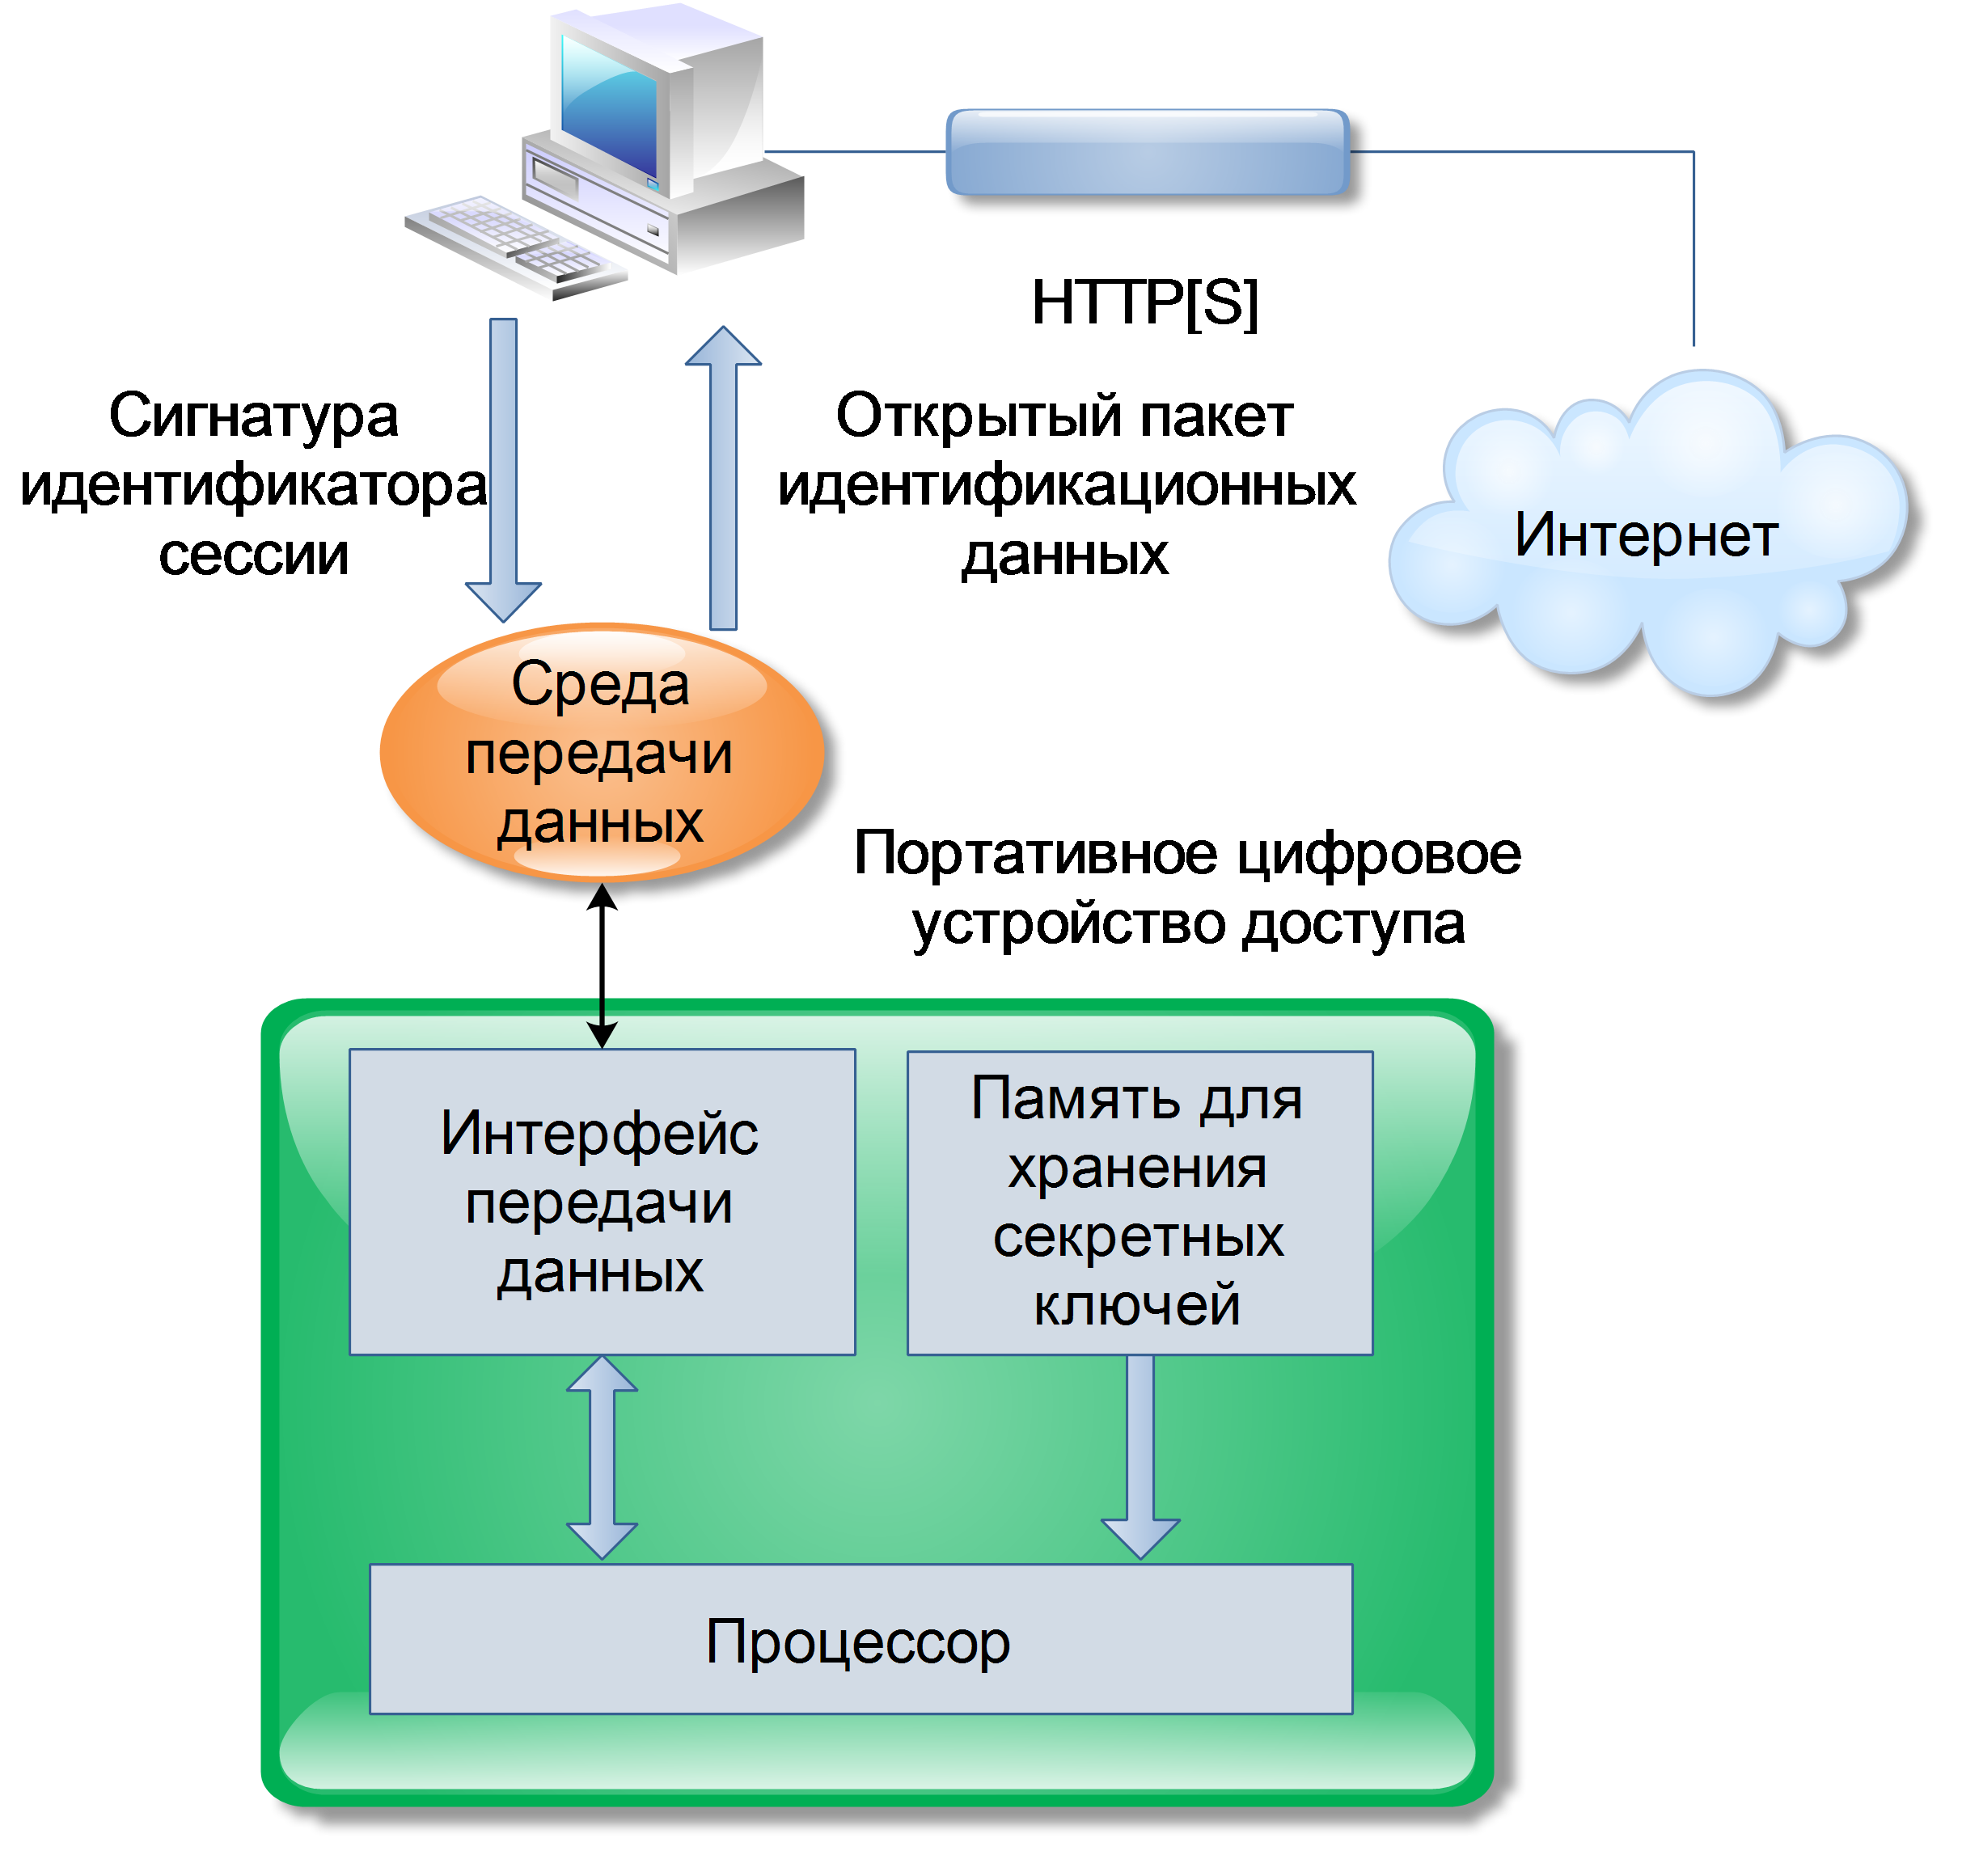
\includegraphics[width=0.7\linewidth]{1-5-1}}
\caption{Концептуальная схема подсистемы аутентификации пользователей}
\label{ris:1.5.1}
\end{figure} 

На основе данных, полученных в результате анализа, можно сформулировать вариант
решения, который позволит устранить недостатки существующих систем доступа.

Исходя из указанных недостатков традиционных подходов к аутентификации, была
предложена новая идея, основанная на использовании портативного
электронного устройства в качестве инструмента доступа к Web-порталу. Процесс
доступа основывается на реализации алгоритмов шифрования.
~\cite{thesis_digit_sign,thesis_smart_card}

Уникальность данной разработки заключается в том, что доступ осуществляется при
помощи специального устройства, способного не только хранить секретные ключи, но
и на их основе вычислять параметры алгоритмов, которые могут далее передаваться
в открытом виде.

Таким образом мастер-ключ алгоритма не копируется на персональный компьютер, где
он сильно уязвим и может быть подвержен атаке. Считывание ключей из устройства
физически неосуществимо в силу ряда принципов работы микроконтроллера, на основе
которого оно построено. Выходные данные алгоритма вычисляются на устройстве и
далее передаются по открытым каналам.

Данное устройство должно быть изготовлено таким образом, чтобы оно соединялось с
персональным компьютером с помощью стандартного интерфейса передачи данных (USB)
без использования дополнительных считывателей. Концептуальная схема данной
технологии представлена на рисунке~\ref{ris:1.5.1}.

Таким образом, с помощью данного устройства достигается механизм двухфакторной
аутентификации. Кроме того, данное устройство можно использовать для
осуществления электронного документооборота применяя технологию
электронно-цифровой подписи.

В качестве области приложения данный программно-аппаратный комплекс можно
рассмотреть в контексте системы управления доступом к распределеной сети
корпоративных порталов.~\cite{conf_itnop_lsa_concept}

\begin{figure}[ht]
\center{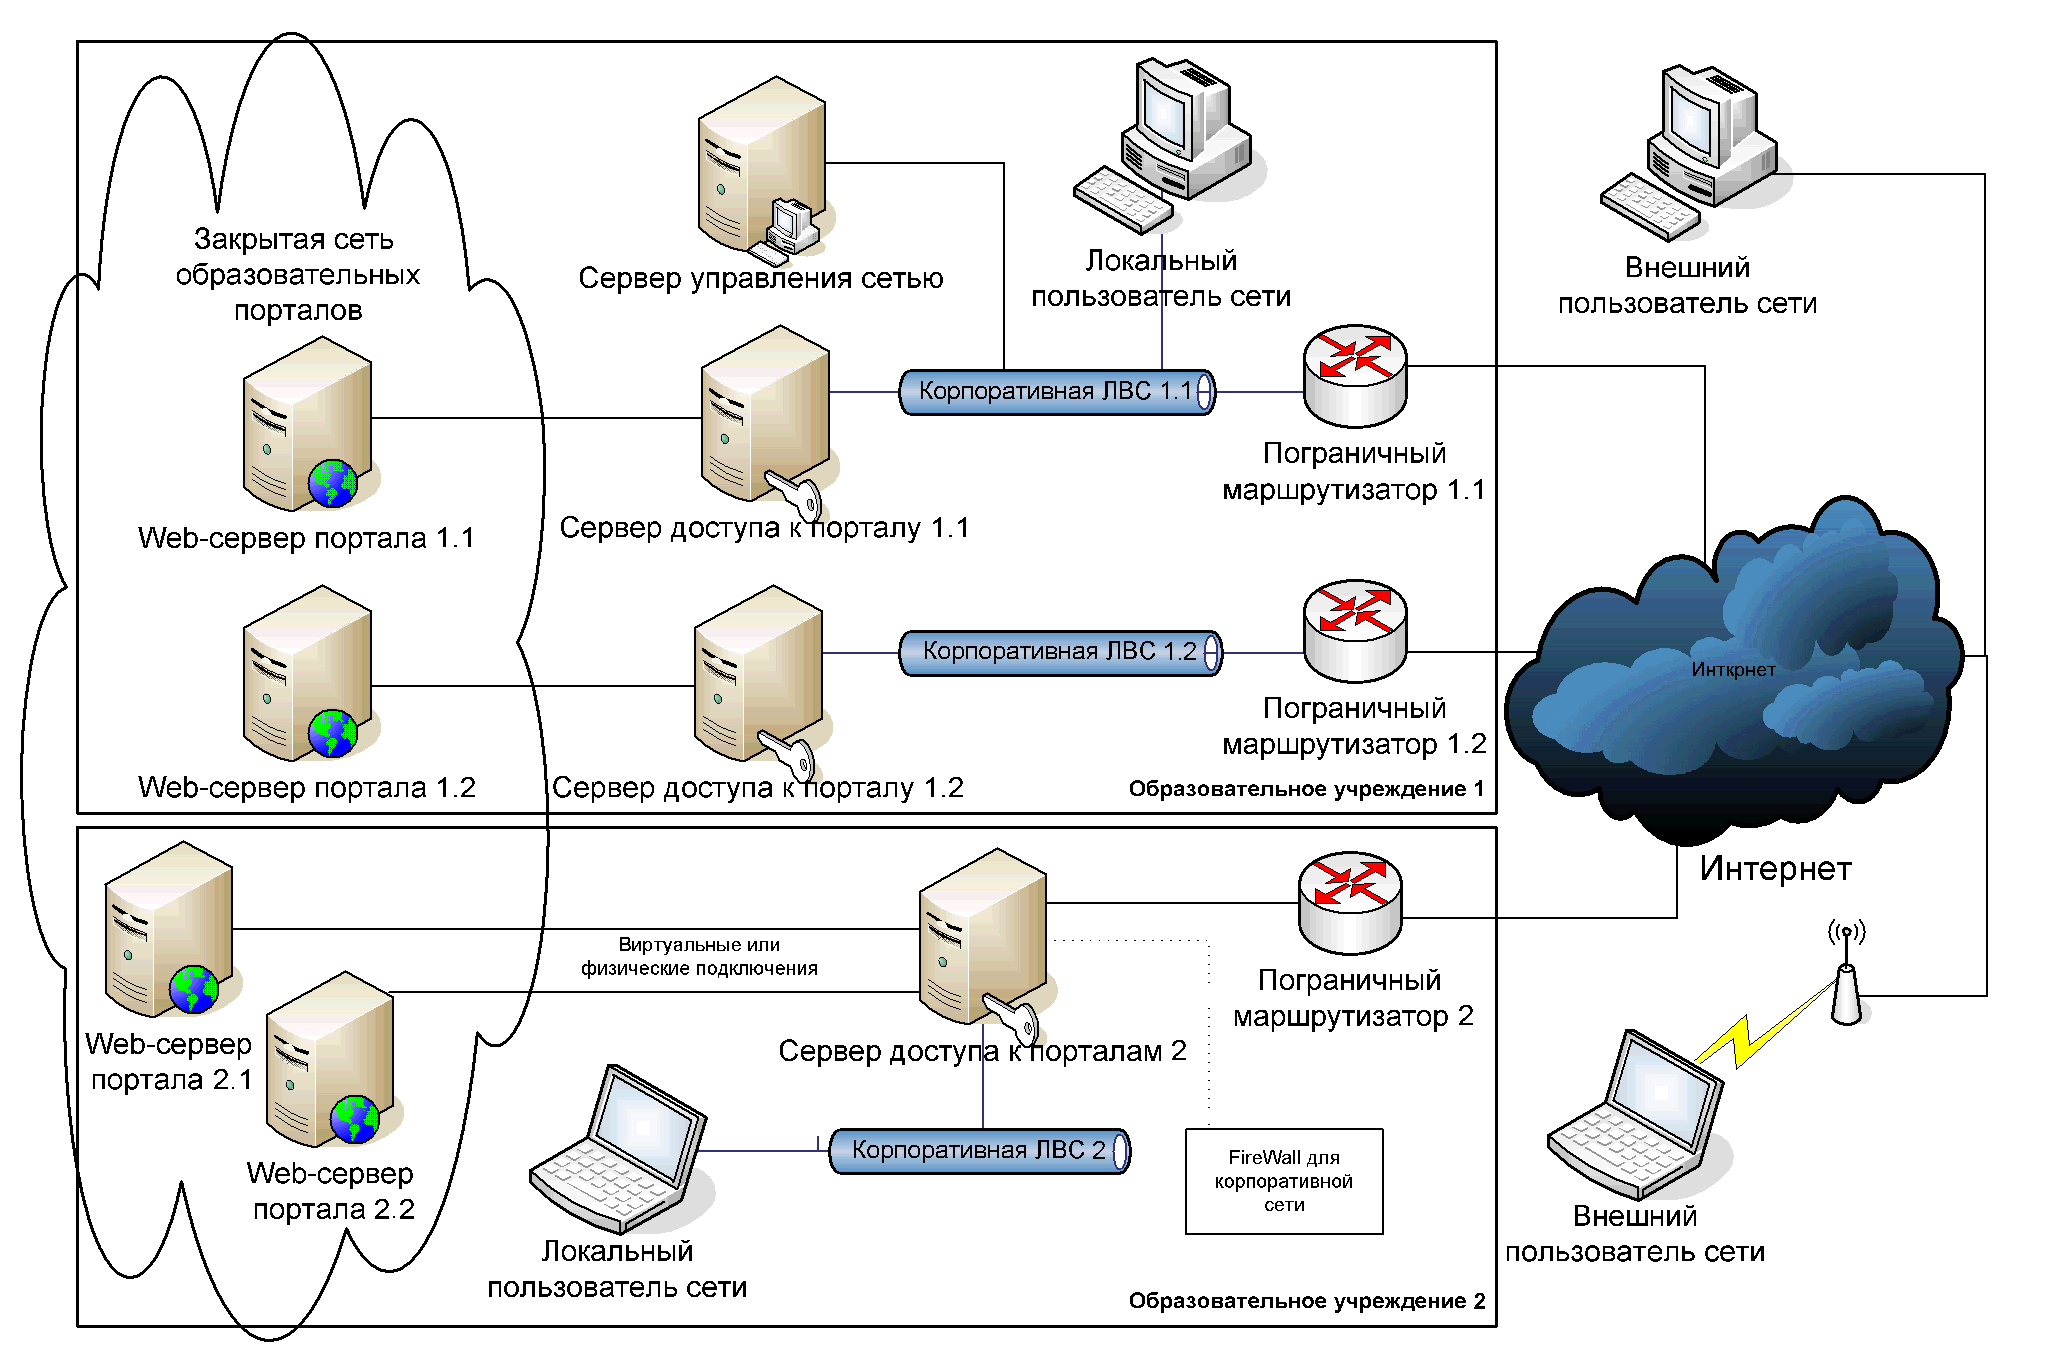
\includegraphics[width=1\linewidth]{1-5-2}}
\caption{Схема развертывания элементов распределенной системы доступа}
\label{ris:1.5.2}
\end{figure} 

Программно-аппаратный комплекс доступа на основе портативных
электронных цифровых ключей предполагает наличие серверной и клиентской части.
Серверная часть представляет собой наборы алгоритмов, которые производят
верификацию сгенерированных шифров со стороны пользователя. Клиентская часть в
свою очередь состоит непосредственно из портативного цифрового устройства
доступа и web-скриптов, загружающихся в браузер клиента через web-страницу и
осуществляющих взаимодействие с ключом.

В результате интеграции в систему управления доступом (беря во внимание схему
на рисунке~\ref{ris:1.5.2}) серверная часть инсталлируется на сервера доступа.
Портативное цифровое устройство доступа подключается к пользовательской машине. Во время
работы устройства синхронизирующие программы подгружаются через web-страницу с
сервера доступа и выполняют информационный обмен с ключом. Таким образом можно
осуществлять аутентификацию пользователя в системе и производить электронный
документооборот, используя электронно-цифровую подпись (ЭЦП).
\chapter{Обоснование эффективности применения разрабатываемой подсистемы}

Разрабатываемую подсистему, из-за своей специфики, можно отнести к классу
открытых систем. Одним из важных признаков таких систем является повышенная безопасность.
~\cite{zapechnikov}

Дадим определения основных понятий, которыми в дальнейшем будем пользоваться при
рассмотрении вопросов защиты.

Под термином \textit{<<информационная безопасность>>}, согласно определению
Гостех-комиссии при Президенте РФ, понимают состояние защищенности информации,
обрабатываемой средствами вычислительной техники или автоматизированной системы,
от внутренних или внешних угроз:
от нежелательного ее разглашения (нарушения конфиденциальности), искажения
(нарушения целостности), утраты или снижения степени доступности информации, а
также ее незаконного тиражирования, которые приводят к материальному или
моральному ущербу владельца или пользователя информации.~\cite{ruk_doc}

\textit{Угрозы (threats)} --- потенциально возможное событие, действие или
процесс, которые посредством воздействия на компоненты системы могут привести к
нанесению ущерба. Это также и люди или группы людей, способные взломать
компьютерную систему.~\cite{gerasimenko} Это может быть любопытный подросток,
рассерженный служащий или шпион конкурирующей компании или иностранного правительства.
Наличие угрозы необязательно означает, что она реализуется и нанесет вред.

\textit{Уязвимость (vulnerability)} --- любая характеристика или свойство
системы, использование которой нарушителем может привести к реализации угрозы. Иными
словами, это слабые места в системах~\cite{gerasimenko}. Уязвимости могут использоваться для
компрометации (взлома) систем.

\textit{Вторжение (intrusion)} --- процесс попытки несанкционированного
проникновения в какую-либо систему. Под вторжением может пониматься любое действие нарушителя,
приводящее к реализации угрозы путем использования уязвимостей. Поэтому это
реализовавшаяся угроза.

\textit{Атака (attack)} --- это событие (момент), при котором злоумышленник
проникает внутрь системы или совершает по отношению к ней какое-либо несанкционированное
действие. Атака является результатом вторжения.

Все нарушители могут быть разделены на две категории:
\begin{enumerate}
  \item Аутсайдеры (outsiders) --- это внешние нарушители по отношению к
  открытой сети, которые атакуют внутренние сетевые ресурсы (цель -- удаление
  информации на корпоративном веб-сqервере, пересылка спэма через почтовый сервер и т.д.). 
  Злоумышленники могут осуществлять атаки из Интернета через модемные линии, через физическое 
  подключение к каналам связи или из сети партнеров (поставщиков, заказчиков, дилеров и т.д.).
  \item Инсайдеры (insiders) --- это внутренние нарушители, находящиеся внутри
  сети и имеющие полный доступ ко всем ее серверам. Это пользователи,
  неправильно применяющие свои привилегии или исполняющие роль
  привилегированного пользователя (например, с привилегированного терминала).
  Исследования показывают, что 80 \% всех атак в сетях исходит именно от
  инсайдеров. Заметим, что существующие методы безопасности не обеспечивают
  защиту от них. Внутренние злоумышленники представляют основную опасность, так
  как они знакомы с системой зашиты, направлением деятельности компании и могут
  реально оценить стоимость ресурсов корпоративной сети. В этой категории опасность 
  представляют уволенные и обиженные сотрудники, мстящие от обиды, <<продвинутые>> 
  пользователи, при каждом удобном случае желающие продемонстрировать свои
  знания, и администраторы, которые в силу своих обязанностей знают многие секреты организации.
\end{enumerate} 

Внутренние злоумышленники по характеру действий могут быть разделены на
следующие категории:
\begin{itemize}
  \item Посторонние лица (у которых права в действующей ИС отсутствуют) осуществляют
перехват или воздействие на информацию, передаваемую по телекоммуникационным
сетям, а также квалифицированное воздействие на систему защиты и работу ИС в
целом с использованием телекоммуникационных сетей.
  \item Разработчики приложений (у которых права в действующей ИС отсутствуют) к уже
названным двум действиям добавляют на этапе разработки ПО реализацию
преднамеренных скрытых возможностей для последующего входа в систему или
непреднамеренных ошибок.
  \item Обслуживающий персонал (у которого права в ИС и на уровне приложений
отсутствуют, но имеется доступ к техническим средствам и ПО) может вести себя
как постронее лицо, плюс получать доступ к сетевому и телекоммуникационному
оборудованию, устанавливать посторонние программы и внедрять программные
закладки.
  \item Пользователи ИС --- сотрудники или клиенты (права на доступ к приложениям ИС)
-- осуществляют перехват или воздействие на информацию, передаваемую по
телекоммуникационным сетям, вносят вредоносное ПО в ИС и присваивают полномочия
других пользователей (в том числе администратора).

В основном их цели сводятся к следующему:
\begin{itemize}
  \item финансовой выгоде;
  \item политической выгоде -- небольшой, но существенный, процент атакующих
  делают это по политическим соображениям, например, они пытаются таким образом
  обратить внимание общественности на отдельную проблему (права животных,
  контроль за оружием, свобода слова и т.д.);
  \item разрушению;
  \item мести недовольных сотрудников;
  \item вызову обществу;
  \item самоутверждению (например, дети хотят поразить друзей своими знаниями и
  навыками);
  \item спорту -- возможно, администратор хвастается защищенностью своего
  интранета, говоря всем, что он непроницаем; перед таким вызовом нарушитель устоять не может;
  \item шутке.
\end{itemize}
\end{itemize}

Угрозы осуществляются на практике в результате стечения случайных обстоятельств
(ошибки, пропуски, сбои электроэнергии, природные бедствия) либо из-за
преднамеренных действий злоумышленников. Общепринятой классификации угроз
безопасности пока не существует.

Возможна классификация угроз безопасности по следующим признакам:
\begin{enumerate}
  \item Цели реализации (цели могут быть связаны, например, со свойствами
  конфиденциальности, целостности и доступности информации, которые собирается
  нарушить злоумышленник, или с расширением прав доступа и получением полного
  контроля над работой компьютера пользователя или определенным сервером);
  \item принципу воздействия на систему (например, взлом парольной защиты или
  нападение на основе сетевого протокола);
  \item характеру воздействия на систему (например, пассивный перехват трафика
  или активная подмена данных);
  \item причине появления используемой ошибки защиты (например, из-за отсутствия
  средств обнаружения вторжений, неправильной настройки средств защиты или не
  установки защищающих обновлений);
  \item объекту атаки (например, данные, программы, сетевое обеспечение);
  \item используемым средствам атаки;
  \item состоянию объекта атаки (например, явное изменение состояния или
  отсутствие каких бы то ни было изменений, так как осуществляется лишь
  пассивный перехват входящих и исходящих пакетов или почтовых сообщений);
  \item по источнику угроз и т. п.
\end{enumerate}

Согласно ставшему уже классическим подходу для информации вообще выделяются три
вида угроз, связанные с ее основными свойствами:
\begin{enumerate}
  \item Угрозы конфиденциальности (конфиденциальность --- защищенность
  информации от несанкционированного ознакомления с нею, подразумевающая
  некоторую классификацию данных, получение либо использование которых
  неавторизованными для этого лицами может стать причиной серьезного ущерба для
  владельцев или пользователей этой информации); примеры угроз: хищение
  (копирование) информации и средств ее обработки, утрата (неумышленная потеря,
  утечка) информации и средств ее обработки.
  \item Угрозы целостности (целостность --- состояние, при котором данные,
  представленные в компьютере, в точности соответствуют данным в исходных
  документах и при этом не могут быть подвержены неумышленным или умышленным
  искажениям или разрушениям; информация может пострадать от сознательных
  действий злоумышленника, от ошибок персонала, от пожара, аварий и др.);
  примеры угроз: модификация (искажение) информации, отрицание ее подлинности,
  навязывание ложной информации.
  \item Угрозы доступности (доступность --- возможность за приемлемое время
  получить требуемую информационную услугу, причем наличие системы безопасности
  не должно создавать помех нормальной работе системы); примеры угроз:
  блокирование информации; уничтожение информации и средств ее обработки.
\end{enumerate}
 
Анализ всего комплекса угроз и оценка последствий их реализации составляет одну
из первых задач сотрудников, ответственных за безопасность. Оценка уязвимости
систем предполагает изучение всех комбинаций реализации перечисленных угроз и
последствий, к которым они приводят. По мере совершенствования средств и методов
защиты компьютерных систем злоумышленниками создаются новые, весьма изощренные
способы их преодоления. Приведем здесь перечень наиболее вероятных случайных
происшествий и злоумышленных действий, которые важны при оценке степени
уязвимости любой системы.
\begin{enumerate}
  \item Происшествия, связанные с техническими причинами:
  \begin{itemize}
    \item выход из строя дискового накопителя с повреждением диска;
	\item отказы, вызванные ошибками в ПО;
	\item повреждение магнитных носителей;
	\item отказы электронных схем компьютеров и периферийного оборудования;
	\item нарушения в сети электропитания: перенапряжение, импульсные выбросы,
аварийное отключение электропитания, воздействие статического электричества;
	\item ошибки при передаче данных по каналам связи;
	\item повреждения кабелей связи при строительных работах. 
  \end{itemize}
  \item Происшествия, связанные со стихийными бедствиями:
  \begin{itemize}
    \item пожар;
	\item затопление при аварии водопровода, отопления или канализации;
	\item разрушение ветхих элементов конструкции здания;
	\item прямое попадание молнии или наводка импульсных токов во время грозы.
  \end{itemize}
  \item Происшествия, связанные с ненамеренными действиями людей:
  \begin{itemize}
    \item случайное заражение компьютера вирусом при использовании посторонней
    программы -- игры, учебного пакета и т. п.;
	\item ошибочные действия малоквалифицированного персонала при профилактике,
техническом обслуживании или ремонте; 
	\item ненамеренное повреждение аппаратуры в результате случайных действий
	безответственных лиц, например, обрыв соединительного кабеля или повреждение
	аппаратуры при неосторожном поведении в помещении, где установлена система;
	\item ошибочные действия оператора при работе, приводящие к разрушению данных;
	\item неправильное обращение с гибкими дисками или другими магнитными
	носителями при их использовании или хранении.
  \end{itemize}
  \item Умышленные действия людей, наносящие вред системе: 
    \begin{itemize}
    \item проникновение в систему через внешний (например, телефонный) канал
    связи с присвоением полномочий одного из легальных пользователей с целью
    подделки, копирования или уничтожения данных (реализуется угадыванием либо
    подбором паролей, выявлением паролей и протоколов через агентуру в
    организации, перехватом паролей при негласном подключении к каналу во время
    сеанса связи, дистанционным перехватом паролей в результате приема
    электромагнитного излучения);
	\item проникновение в систему через телефонную сеть при перекоммутации канала
	на модем злоумышленника после вхождения легального пользователя в связь и
	предъявления им своих полномочий с целью присвоения прав этого пользователя на
	доступ к данным;
	\item копирование информации и паролей при негласном пассивном подключении к
	кабелю сети или при приеме электромагнитного излучения сетевого адаптера; 
	\item выявление паролей легальных пользователей при негласном активном
	подключении к коммуникационной сети при имитации запроса сетевой ОС; 
	\item анализ трафика при пассивном подключении к каналу связи (с помощью так
	называемых снифферов, перехватчиков, от англ. sniffer) или при перехвате
	электромагнитного излучения аппаратуры для выявления протоколов обмена;
	\item подключение к каналу связи в качестве активного ретранслятора для
	фальсификации документов, изменения их содержания, порядка следования,
	повторной передачи, доставки с задержкой или упреждением;
	\item блокировка канала связи собственными сообщениями, вызывающая отказ в
	обслуживании легальных пользователей; отказ абонента от факта приема (передачи)
	документов или формирование ложных сведений о времени приема (передачи)
	сообщений для снятия с себя ответственности за выполнение этих операций;
	\item формирование ложных утверждений о полученных (переданных) документах;
	\item скрытая несанкционированная передача конфиденциальной информации в
	составе легального сообщения для выявления паролей, ключей и протоколов доступа; 
	\item незаконное объявление пользователем себя другим пользователем
	(маскировка) для нарушения адресации сообщений или возникновения отказа в
	законном обслуживании;
	\item сбор и анализ использованных распечаток, документации и других материалов
	для копирования информации или выявления паролей, идентификаторов, процедур
	доступа и ключей;
	\item визуальный перехват информации, выводимой на экран дисплеев или вводимой
	с клавиатуры для выявления паролей, идентификаторов и процедур доступа;
	\item негласная переработка оборудования или ПО на фирме-изготовителе,
	фирме-поставщике, в месте складирования или в пути следования к заказчику с
	целью внедрения средств НСД к информации извне (программ-перехватчиков и
	<<троянских коней>>, аппаратуры вывода информации и т.п.), а также уничтожение
	информации или оборудования (например, с помощью вирусов, ликвидаторов с
	дистанционным управлением или замедленного действия и т.п.);
	\item разрушение информации или создание сбоев в сети с помощью вирусов для
дезорганизации деятельности организации (реализуется загрузкой вирусов в
нерабочее время, подменой игровых программ, используемых сотрудниками в рабочих
помещениях, или вручением сотруднику <<подарка>> в виде новой компьютерной игры
или другой занимательной программы);
	\item похищение оборудования, в том числе отдельных плат, дисководов,
	дорогостоящих микросхем, кабелей, дисков, лент, с целью продажи, что влечет за
	собой потерю работоспособности системы, а иногда и уничтожение данных;
	\item похищение магнитных носителей с целью получения доступа к данным и
	программам; 
	\item разрушение оборудования, магнитных носителей или дистанционное стирание
	информации (например, с помощью магнитов); 
	\item считывание информации с жестких и гибких дисков (в том числе и остатков
	<<стертых>> файлов), магнитных лент при копировании данных с оборудования на
	рабочих местах в нерабочее время, при копировании данных с использованием
	терминалов, оставленных без присмотра в рабочее время; копирование данных с
	магнитных носителей, оставленных на столах или в компьютерах; копирование
	данных с оборудования и магнитных носителей, убранных в специальные хранилища,
	при их вскрытии или взломе;
	\item внесение изменений в данные и программы для подделки и фальсификации
	документов при включении системы во время негласного посещения в нерабочее время; 
	\item использование оставленного без присмотра оборудования в рабочее время;
	внесение изменений в данные, записанные на оставленных без присмотра магнитных носителях; 
	\item установка скрытых передатчиков для вывода паролей с целью копирования
	данных или доступа к ним по легальным каналам связи с сетью в результате
	негласного посещения в нерабочее время, посещения с целью ремонта, настройки,
	профилактики оборудования или отладки ПО, скрытой подмены элементов
	оборудования при оставлении их без присмотра в рабочее время;
	\item установка ликвидаторов замедленного действия или с дистанционным
	управлением (программных, аппаратных или аппаратно-программных с исполнительным
	механизмом взрывного, химического, электрического или вирусного действия) с
	целью уничтожения информации или оборудования; 
	\item несанкционированное изменение
	своих полномочий на доступ или полномочий других пользователей в обход
	механизмов защиты;
	\item внесение изменений в базу данных или в отдельные файлы в пределах
	выделенных полномочий для подделки или уничтожения информации.
  \end{itemize}
\end{enumerate}

Анализ угроз должен включать в себя:
\begin{itemize}
  \item оценку характера и ценности информации, хранящейся в системе;
  \item построение модели злоумышленника, т.е. оценку того, от кого нужно
  защищаться -- от постороннего лица, пользователя системы, администратора и
  т.д.;
  \item выделение наиболее опасных угроз для хранящейся в системе информации
(несанкционированное чтение или изменение и т.д.); 
  \item оценку затрат времени и средств на вскрытие системы, необходимых для
злоумышленников; 
  \item оценку допустимых затрат времени, средств и ресурсов системы на
организацию ее защиты.
\end{itemize}

При анализе угроз, вызванных злоумышленными действиями, целесообразно выяснить
их мотивы, цели и последствия, а также определить круг потенциальных инициаторов
(субъектов) таких действий. Основными нарушителями могут быть, например,
сотрудники (нынешние и бывшие) и клиенты организации, конкуренты и конкуренты клиентов.
Согласно статистике компьютерных преступлений основным их мотивом оказывается
незаконное обогащение, а чаще всего в качестве субъектов преступлений выступают
сотрудники (бывшие сотрудники). Значительно реже встречаются такие причины, как
месть обиженных сотрудников или завоевание престижа среди определенной группы
лиц.~\cite{zapechnikov}

При анализе способов осуществления злоумышленных действий следует различать
субъекта действий и конкретных исполнителей. Так, для шпионажа или диверсии в
роли агентов выступают сотрудники банка, его клиенты, обслуживающий персонал из
внешних организаций, просто посторонние, т.е. все те лица, которые могут
получить доступ к сети или его элементам.
По характеру исполнения злоумышленные действия делятся на три вида:
\begin{enumerate}
  \item Действия, не связанные с проникновением исполнителей в помещения, где
  расположены компоненты сети;
  \item Действия с единичными проникновениями исполнителей в помещения:
  \begin{itemize}
    \item открытые -- под видом посетителей, сотрудников коммунальных служб
    (уборщики, водопроводчики, телефонисты, электрики) и т.п.;
	\item негласные -- в выходные дни или ночью;
  \end{itemize}
  \item Действия, которые предусматривают наличие исполнителей в среде
  сотрудников, клиентов или поставщиков оборудования, постоянно работающих в
  помещениях, а также постоянного обслуживающего персонала.
\end{enumerate}        
\section{Уязвимость архитектуры клиент-сервер} 

В основе общения по открытым сетям лежит технология клиент-сервер. Определений
этой архитектуры очень много. В общем случае это такой способ проектирования ИС,
при котором она может быть рассмотрена как совокупность некоторого числа систем
двух видов -- клиентской и серверной.
Как уже отмечалось выше, клиентская часть системы инициирует запросы, а
серверная обрабатывает запросы и при необходимости генерирует ответы клиенту. В
общем случае серверная часть состоит из нескольких элементов --- ОС, СУБД,
прикладной системы, в которой реализована общая бизнес-логика для всех клиентов.
ОС предоставляет необходимые сервисные возможности и программные интерфейсы API
для СУБД, которая в своей БД обрабатывает и выполняет запросы прикладной
системы.~\cite{ComputerWeek}

Угрозы в сетевой среде можно разделить на следующие виды:
\begin{itemize}
  \item прослушивание сети;
  \item изменение корпоративных потоков данных;
  \item воздействие на инфраструктурные сетевые сервисы;
  \item подделка сетевых пакетов;
  \item генерация и посылка аномального трафика (пакетов);
  \item отказ от совершенных действий.
\end{itemize}
	
Прослушивание сети может предприниматься злоумышленниками для достижения следующих целей:
\begin{itemize}
  \item перехвата пересылаемых сведений;
  \item перехвата аутентификационной информации;
  \item анализа трафика.
\end{itemize}
	
Изменение корпоративных потоков данных влечет за собой следующие нарушения
безопасности:
\begin{itemize}
  \item кражу, переупорядочение, дублирование информации;
  \item изменение и вставку собственных данных (нелегальный посредник).
\end{itemize}
	
Воздействие на инфраструктурные сетевые сервисы означает:
\begin{itemize}
  \item вмешательство в работу сервиса имен;
  \item изменение маршрутов корпоративных потоков информации.
\end{itemize}
	
Подделка сетевых пакетов может принимать следующие формы:
\begin{itemize}
  \item подделка адресов;
  \item перехват соединений;
  \item имитация работы других серверов.
\end{itemize}
	
Генерация и посылка аномальных пакетов представляют собой атаки на доступность,
получившие в последнее время относительно широкое распространение.
Наконец, отказ от совершенных действий --- это угроза прикладного уровня, она
реальна в первую очередь в силу распределенности систем клиент-сервер.
~\cite{ComputerWeek} Список наиболее очевидных угроз в архитектуре клиент-сервер выглядит
следующим образом:
\begin{itemize}
  \item пассивный перехват передаваемых запросов;
  \item модификация (активный перехват) передаваемых запросов;    
  \item пассивный перехват ответов клиенту;
  \item модификация ответов клиенту;
  \item выдача злоумышленником себя за определенный сервер;
  \item выдача злоумышленником себя за определенного клиента;
  \item перегрузка сервера выдачей большого числа случайных запросов, что может
привести к отказу обслуживания новых клиентов; 
  \item случайные сбои и ошибки функционирования аппаратуры и программных
  элементов сервера; 
  \item злоумышленные действия зарегистрированных клиентов;
  \item другие виды атак на ПО сервера.
\end{itemize} 
\section{Уязвимость операционных систем} 

Внутренняя структура современных ОС чрезвычайно сложна, поэтому проводить
адекватную политику безопасности и защищать ее гораздо труднее, чем в случае
СУБД. Это обусловлено большим числом различных типов защищаемых объектов и
информационных потоков в современных ОС. Операционная система имеет сложную
внутреннюю структуру и поэтому задача построения адекватной политики
безопасности для ОС решается сложнее, чем для СУБД.
Наилучшие результаты атак достигаются при использовании самых простых методов
взлома через выявленные лазейки в защите ОС -- чем проще алгоритм атаки, тем
больше вероятность того, что атака пройдет успешно. Возможность практической
реализации той или иной атаки на ОС в значительной мере определяется
архитектурой и конфигурацией ОС. Но есть атаки, которые могут быть применены
практически к любой ОС.~\cite{zapechnikov}

\begin{enumerate}
  \item Кража пароля:
  \begin{itemize}
    \item подглядывание за легальным пользователем, когда тот вводит пароль
    (даже если во время ввода пароль не высвечивается на экране, его можно легко
    узнать, следя за перемещением пальцев пользователя по клавиатуре);
	\item получение пароля из файла, в котором он был сохранен <<ленивым>>
	пользователем, не желающим каждый раз затруднять себя вводом пароля при сетевом
	подключении (как правило, такой пароль хранится в незашифрованном виде);
	\item  поиск пароля, записанного на календаре, в записной книжке или на
	оборотной стороне компьютерной клавиатуры (особенно часто подобная ситуация
	встречается, когда администратор заставляет пользователей применять длинные,
	трудно запоминаемые пароли);
	\item кража внешнего носителя парольной информации (дискеты или электронного
	ключа, на которых хранится пароль пользователя для входа в ОС); перехват пароля
	программной закладкой.
  \end{itemize}	
  \item Подбор пароля:
  \begin{itemize}
    \item полный перебор всех возможных вариантов пароля (метод <<грубой
    силы>>);
	\item оптимизированный перебор вариантов пароля: по частоте встречаемости
	символов, с помощью словарей наиболее часто встречающихся паролей, с
	привлечением знаний о конкретном пользователе, с использованием сведений о
	существовании эквивалентных паролей -- тогда из каждого класса эквивалентности
	опробуется всего один пароль, что значительно сокращает время перебора.
  \end{itemize}
  \item Сканирование <<жестких>> дисков компьютера: 
  \begin{itemize}
    \item злоумышленник последовательно
пытается обратиться к каждому файлу, хранимому на <<жестких>> дисках
пользователей сети (если объем дискового пространства достаточно велик, можно
быть вполне уверенным, что при описании доступа к файлам и каталогам
администратор допустил хотя бы одну ошибку, в результате чего все такие каталоги
и файлы будут прочитаны взломщиком);
    \item чтобы скрыть следы, злоумышленник может выступать под чужим именем --
  например, под именем легального пользователя, чей пароль ему известен.    
  \end{itemize}
  \item Сборка <<мусора>> с дисков компьютера и в оперативной памяти: 
  если средства ОС позволяют восстанавливать ранее удаленные объекты,
  злоумышленник может получить доступ к объектам, удаленным другими
  пользователями, просмотрев содержимое их <<мусорных корзин>>.
  \item Превышение полномочий, т.е. используя ошибки в ПО или в
  администрировании ОС, злоумышленник получает полномочия, превышающие те,
  которые предоставлены ему согласно действующей политики безопасности:
  \begin{itemize}
    \item запуск программы от имени пользователя, имеющего необходимые
    полномочия, или в качестве системной программы (драйвера, сервиса, демона и
    т. д.), выполняющейся от имени ОС;
	\item подмена динамически загружаемой библиотеки, используемой системными
	программами, или изменение переменных среды, описывающих путь к таким
	библиотекам; 
	\item модификация кода или данных подсистемы защиты ОС.
  \end{itemize}

  \item Отказ в обслуживании (целью этой атаки является частичный или полный
  вывод ОС из строя):
  \begin{itemize}
    \item захват ресурсов, т.е. программа злоумышленника производит захват всех
    имеющихся в ОС ресурсов, а затем входит в бесконечный цикл;
	\item бомбардировка запросами -- программа злоумышленника постоянно направляет
	ОС запросы, реакция на которые требует привлечения значительных ресурсов сети;
	\item использование ошибок в ПО или администрировании.~\cite{zapechnikov}
  \end{itemize}

\end{enumerate} 
\section{Обобщенная схема уязвимости системы аутентитфикации при различных
подходах к обеспечению безопасности}

Рассмотрев и классифицировав всевозможные виды уязвимостей различных узлов
открытых систем, а так же разновидности атак злоумышленников, построим
обобщенную схему уязвимости системы аутентификации пользователей в сети при
традиционном подходе, указав градации степени стойкости к вредоносным атакам
(Рис.~\ref{ris:2.1}).

\begin{figure}[h]
\center{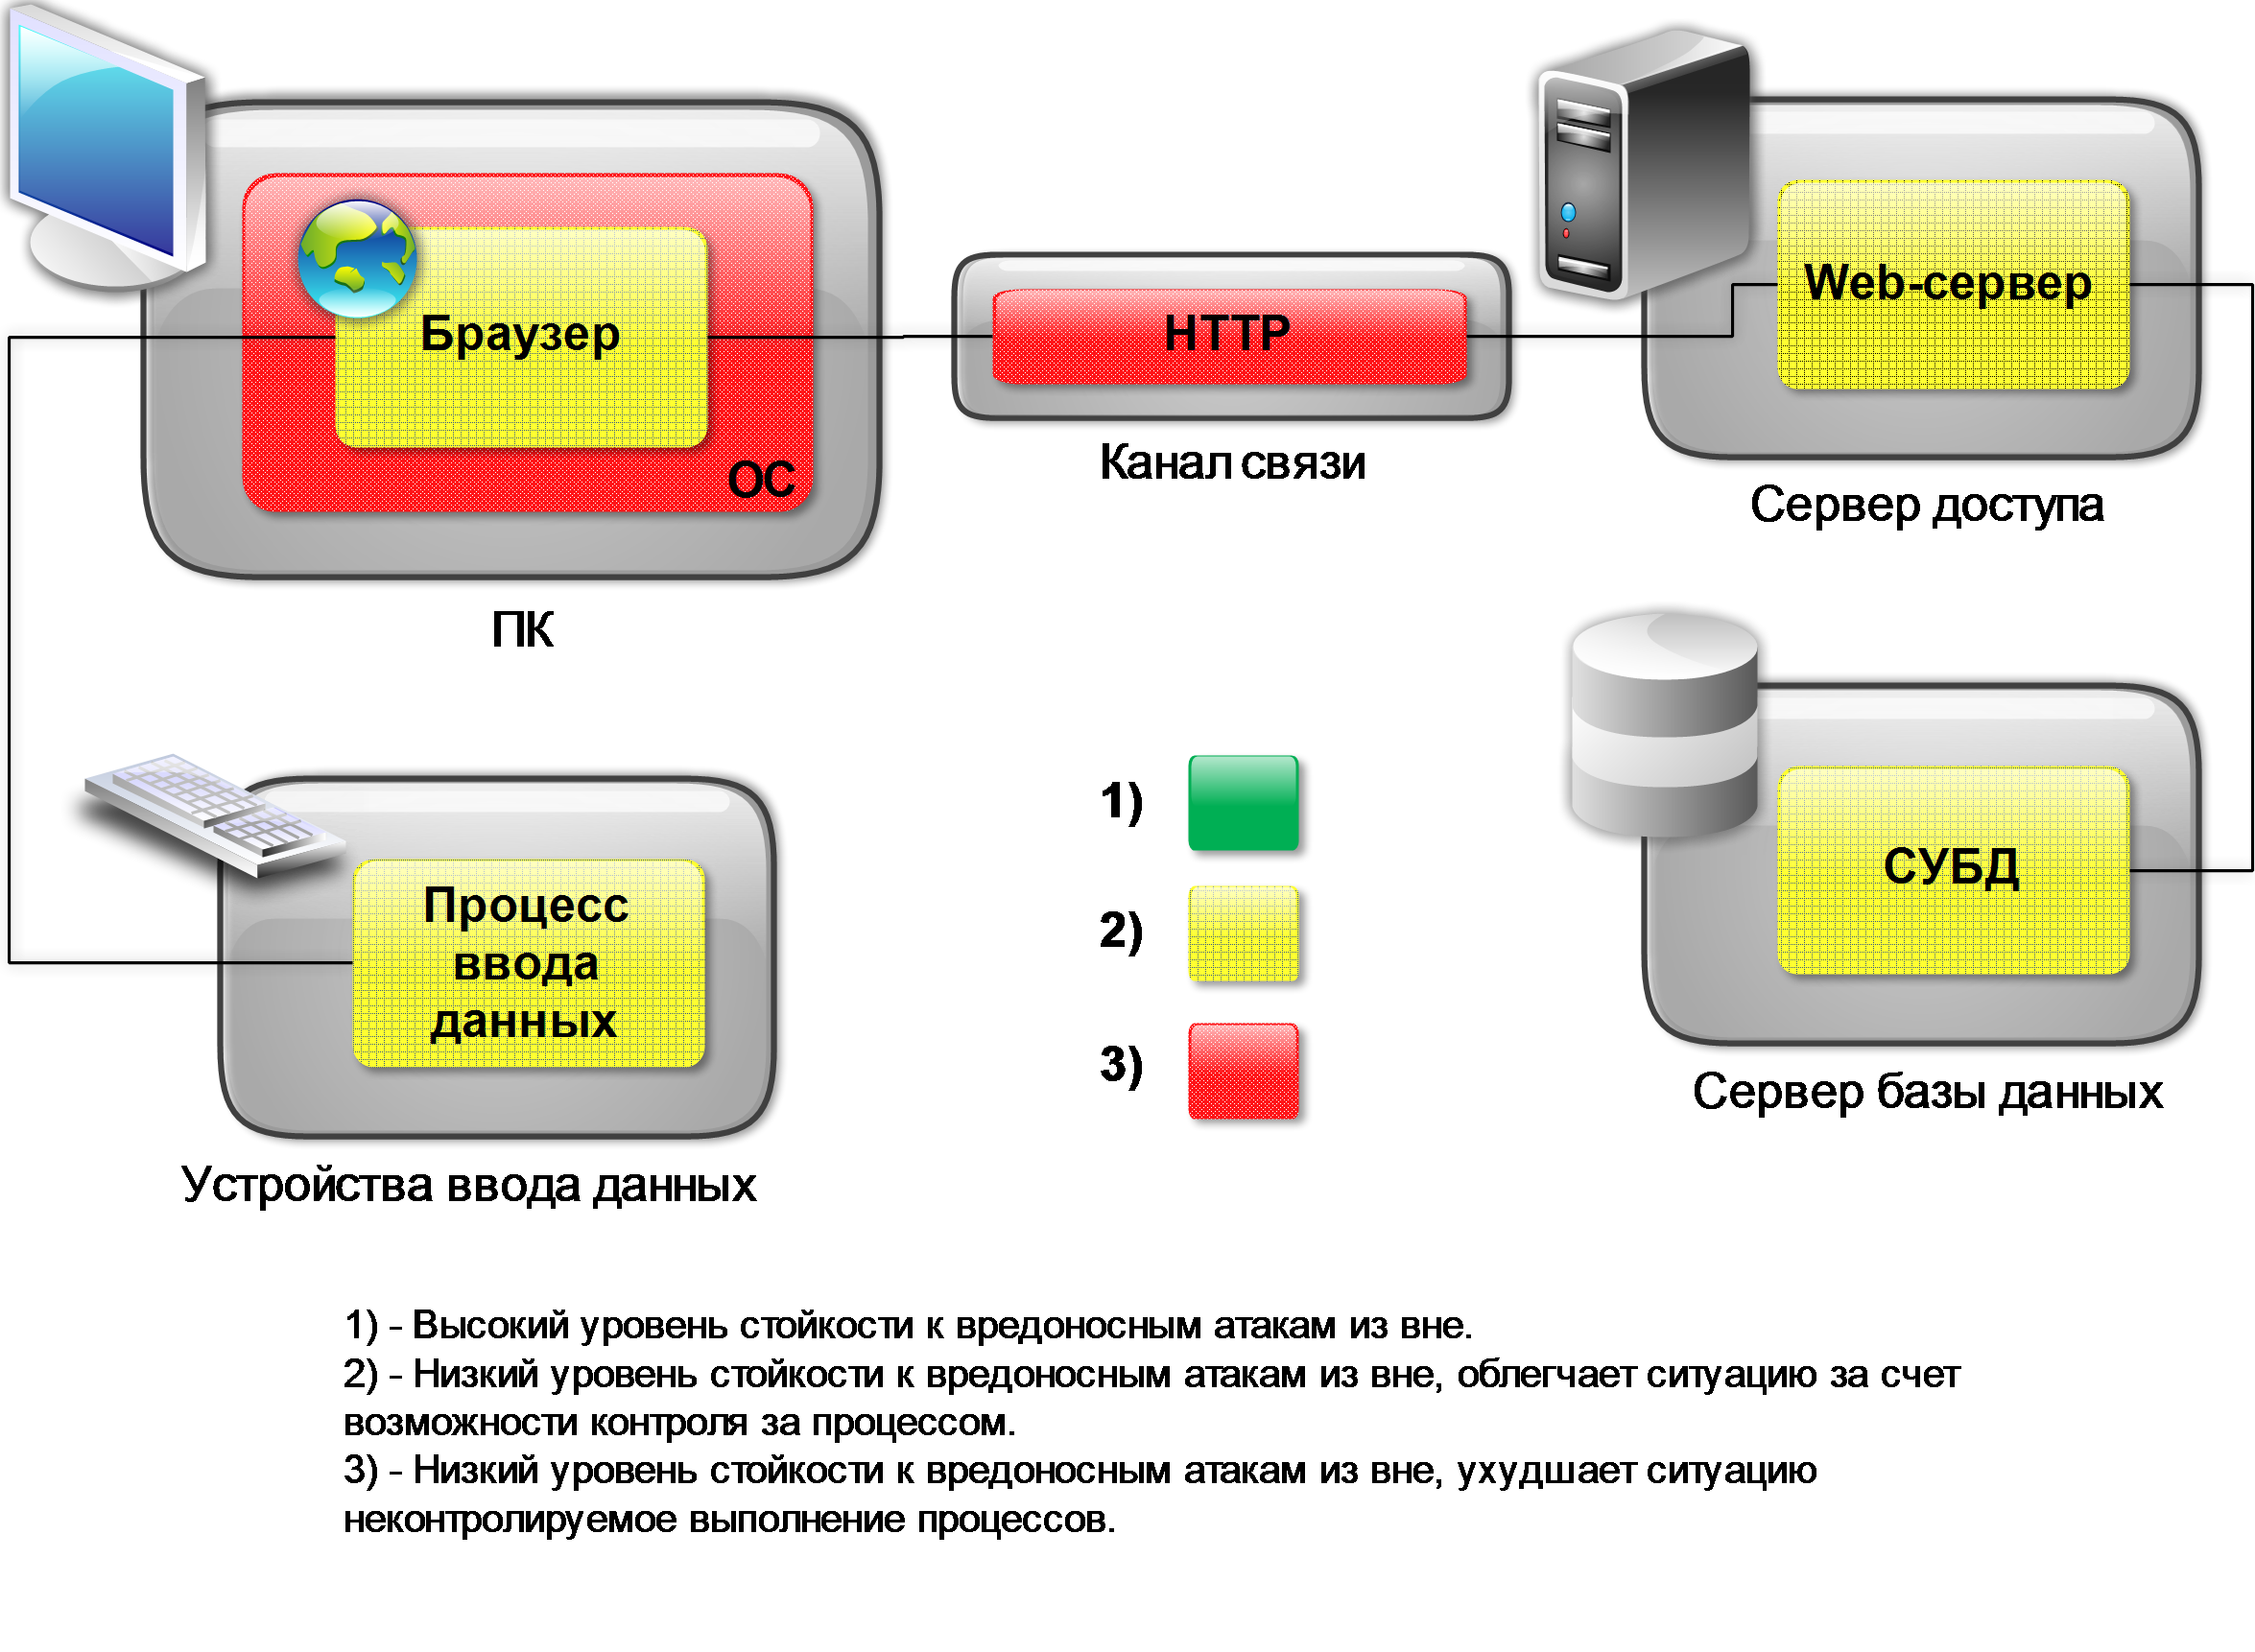
\includegraphics[width=1\linewidth]{2-1}}
\caption{Схема уязвимости узлов системы при традиционном подходе к
процессу аутентификации}
\label{ris:2.1}
\end{figure}

Детально рассмотрим уязвимости, которым подвержен каждый элемент системы в
отдельности.

\textit{Устройства ввода данных}, как правило, представляет собой клавиатуру. В
процессе аутентификации клавиатура может быть использована при вводе пароля. Данное
устройство включено в группу риска по следующим причинам:
\begin{itemize}
  \item данные (в частности пароль), вводимые с клавиатуры, могут быть
  доступными третьему лицу в результате банального слежения за процессом ввода;
  \item в результате целенаправленных действий злоумышленника клавиатура может
  быть сопряжена со специальным прослушивающим устройством, которое фиксирует
  все вводимые данные.
\end{itemize}

\textit{Персональный компьютер} входить в группу повышенной опасности из за
уязъвимостей операционных систем. В частности, угрозы могут исходить из
хаккерских атак, а так же от различных вредоносных программ, целенаправленно
собирающих секретную информацию. Ситуация осложняется из-за
неконтролируемого выполнения процессов, что не дает возможности определить
источник угрозы на ранних этапах.

\textit{Канал связи} является наиболее уязвимым местом любой системы, так как
информация передается абсолютно открытым образом, где практически каждый может
получить к ней доступ.

\textit{Серверная часть системы} так же включена в группу риска, не смотря на
высокие возможности обеспечения безопасности. Любая атака со стороны
злоумышленников может привести к полному отказу в работе системы и необратимым
последствиям.

Применение нового подхода к процессу аутентификации пользователей в сети с
использованием портативного цифрового ключа доступа снижает уровень уязвимости в
отдельных компонентах системы, особенно это касается критических участков. Это
можно проследить на рисунке~\ref{ris:2.2}).

 \begin{figure}[h]
\center{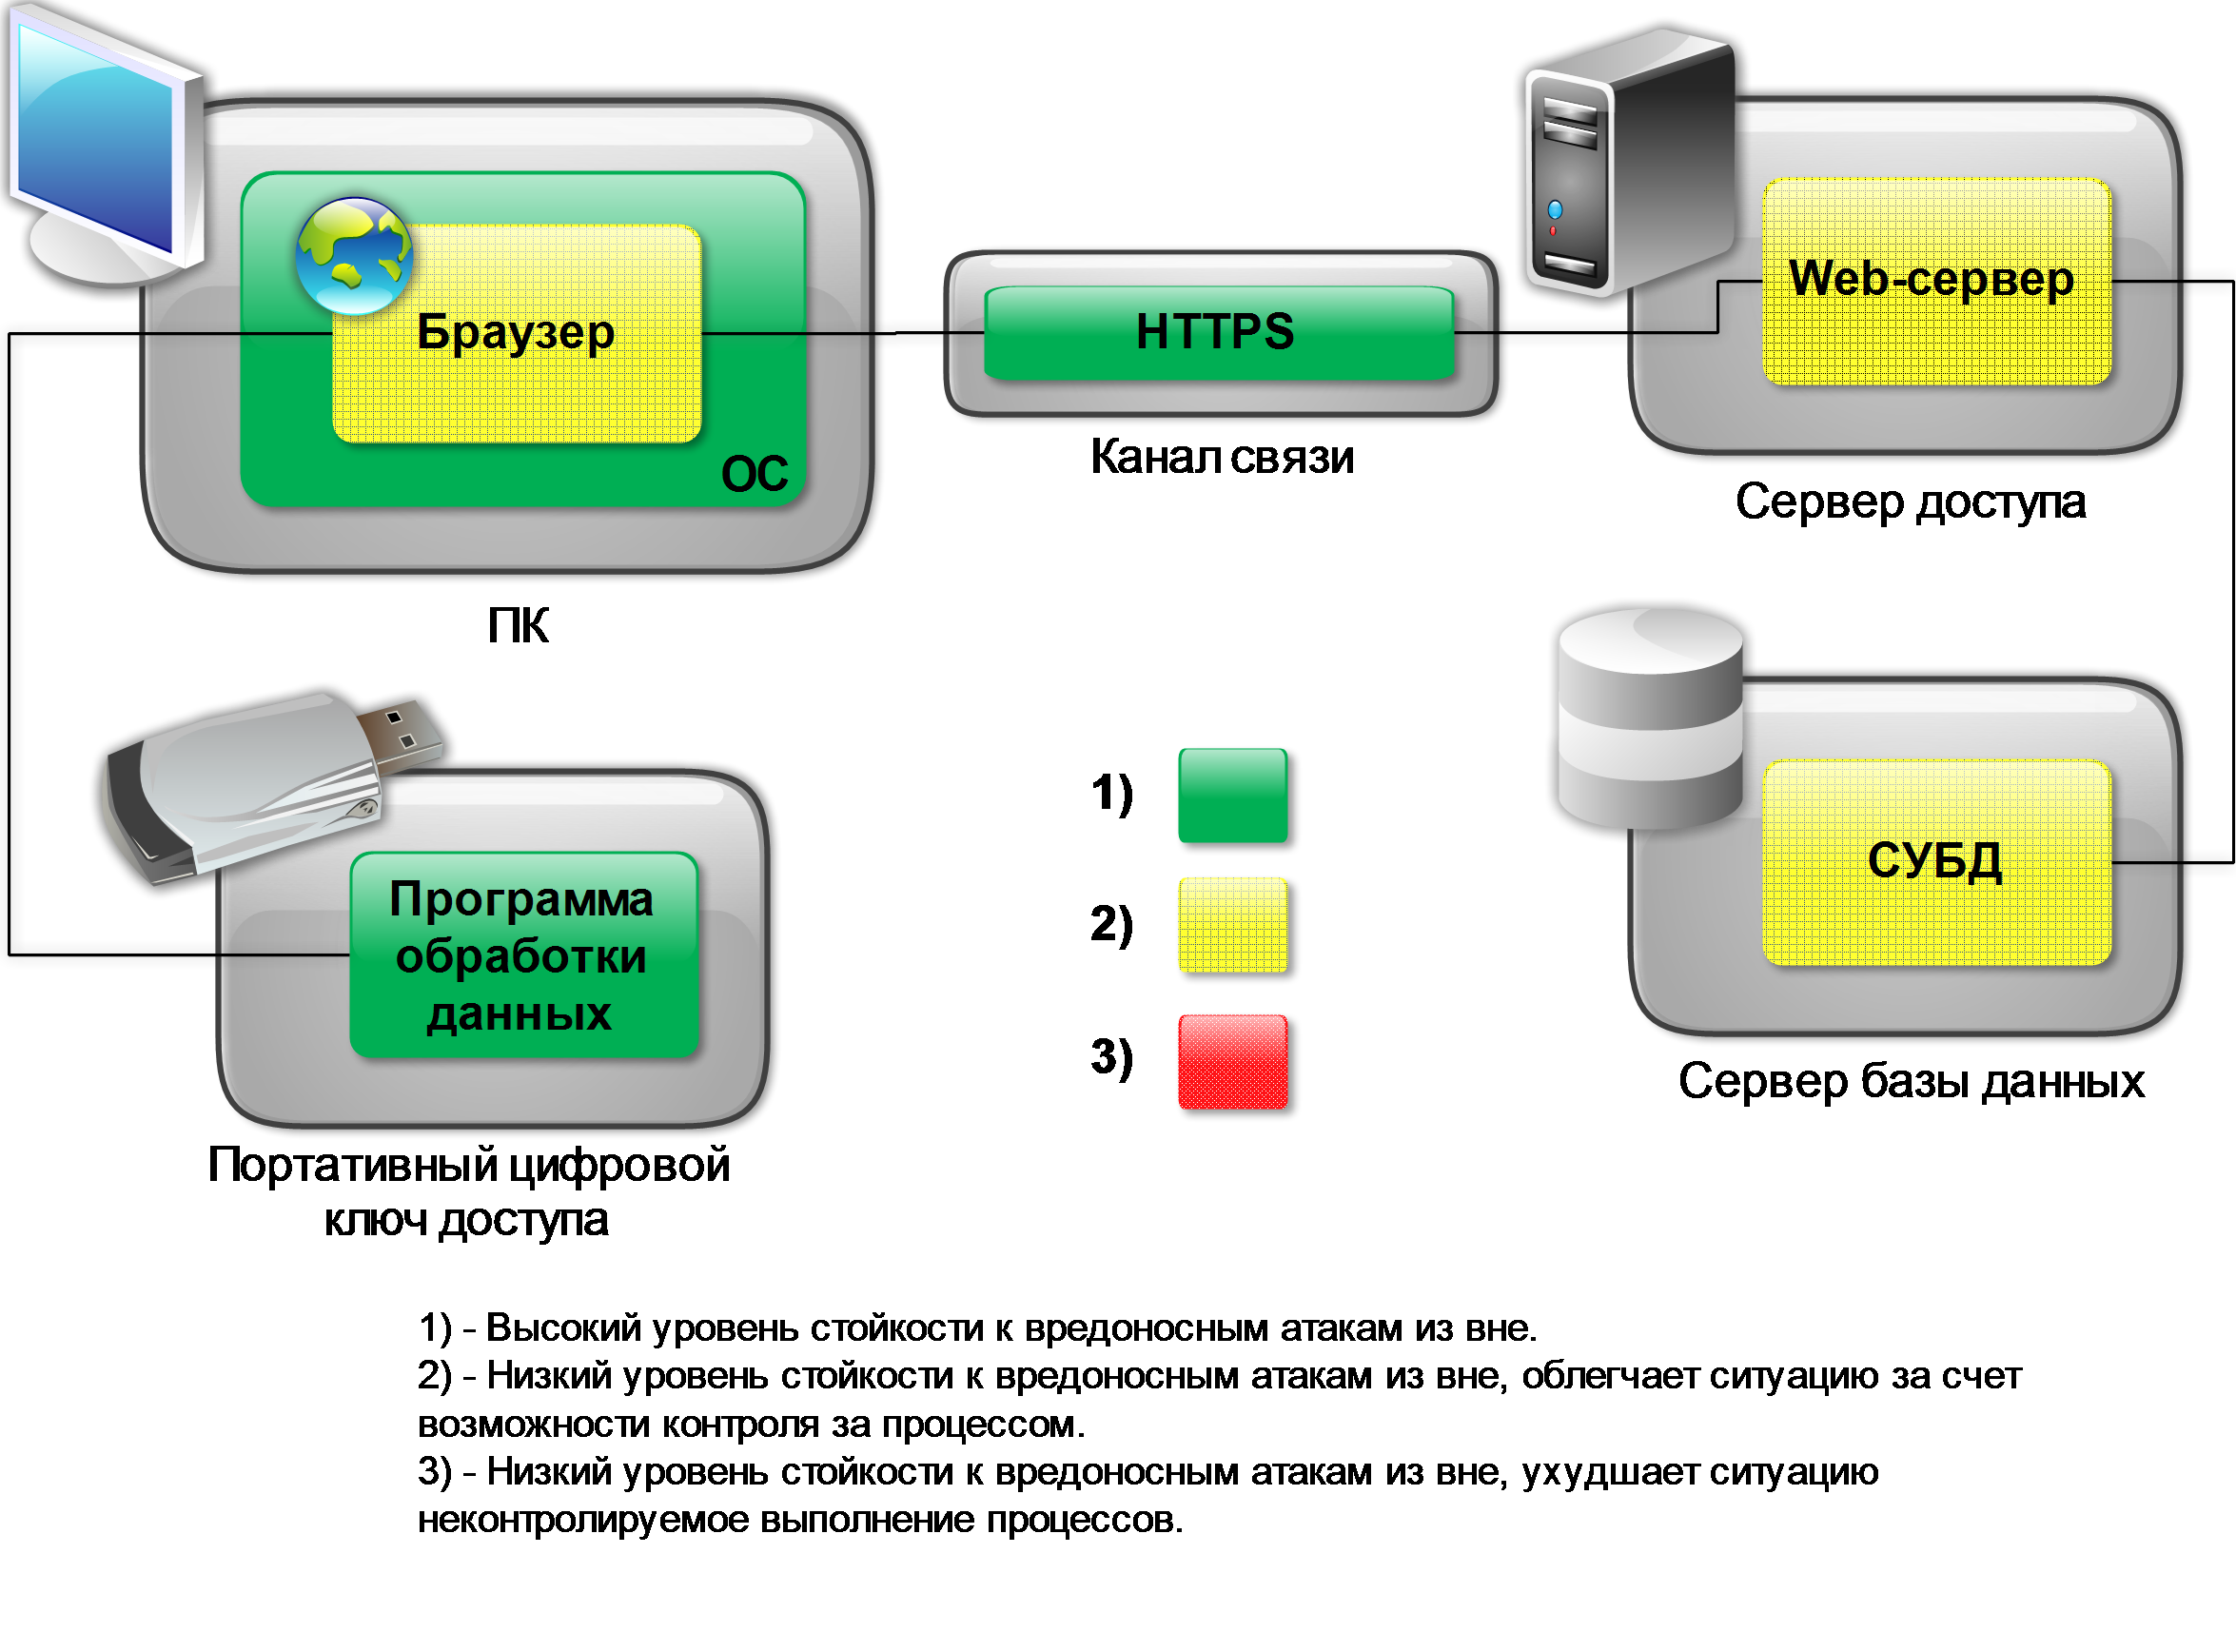
\includegraphics[width=1\linewidth]{2-2}}
\caption{Схема уязвимости узлов системы при новом подходе к процессу аутентификации}
\label{ris:2.2} 
\end{figure}


Выявленные улучшения достигаются с помощью:
\begin{itemize}
  \item Применяемых алгоритмов шифрования данных;
  \item Применения новой технологии хранения ключей и обработки алгоритмов
шифрования.
\end{itemize}

Применяемые алгоритмы шифрования обеспечивают безопасность передаваемых данных
при условии полной секретности ключей. 
  
Алгоритмы шифрования можно разделить на две категории:
\begin{itemize}
  \item алгоритмы симметричного шифрования;
  \item алгоритмы асимметричного шифрования.
\end{itemize}
	
В алгоритмах \textit{симметричного шифрования} для расшифрования обычно
используется тот же самый ключ, что и для зашифрования, или ключ, связанный с ним каким-либо
простым соотношением. Последнее встречается существенно реже, особенно в
современных алгоритмах шифрования. Такой ключ (общий для зашифрования и
расшифрования) обычно называется просто ключом шифрования.
Одним из наиболее распространенных алгоритмов данного вида является 
\textbf{DES} -- федеральный стандарт шифрования США в 1977-2001 годах,
разработанный группой под руководством доктора У. Тачмена. Архитектурой данного
алгоритма является классическая сбалансированная сеть Файстеля с начальной и
конечной битовыми перестановками общего вида. Длина ключа данного алгоритма
составляет 56 бит.

В \textit{асимметричном шифровании} ключ зашифрования $k_{1}$ легко вычисляется
из ключа $k_{2}$ таким образом, что обратное вычисление невозможно. Например, соотношение
ключей может быть таким:
\begin{equation}
k_{1} = a^{k_{2}} \ mod \ p ,
\end{equation}

где $a$ и $p$ -- параметры алгоритма шифрования, имеющие достаточно большую
размерность.

Яркими примерами данного вида шифрования являются алгоритмы \textbf{RSA} и
\textbf{ElGamal}.
Алгоритм RSA - Защищен патентом США N 4405829. Разработан в 1977 году в
Массачусетском технологическом институте (США). Получил название по первым
буквам фамилий авторов (Rivest, Shamir, Adleman). Криптостойкость основана на
вычислительной сложности задачи разложения большого числа на простые множители.
Алгоритм ElGamal разработан в 1985 году. Назван по фамилии автора - Эль-Гамаль.
Используется в стандарте США на цифровую подпись DSS (Digital Signature
Standard). Криптостойкость основана на вычислительной сложности задачи
логарифмирования целых чисел в конечных полях.~\cite{elgamal}

Еще одной разнавидностью асимметричных алгоритмов шифрования является
\textit{алгоритм электронно-цифровой подписи} (ЭЦП). Электронная подпись (ЭП) —
информация в электронной форме, которая присоединена к другой информации в электронной форме
(подписываемой информации) или иным образом связана с такой информацией и
которая используется для определения лица, подписывающего информацию.~\cite{FZ_63}
По своему существу электронная подпись представляет собой реквизит электронного
документа, позволяющий установить отсутствие искажения информации в электронном
документе с момента формирования ЭП и проверить принадлежность подписи владельцу
сертификата ключа ЭП. Значение реквизита получается в результате
криптографического преобразования информации с использованием закрытого ключа
ЭП.

Все существующие алгоритмы ЭЦП построены по единому принципу.
Разница заключается лишь в математической реализации отдельно взятого алгоритма.
Это связано с тем, что каждый новый алгоритм получает улучшения, по двум
основным направлениям:
повышение криптостойкости и снижение временных затрат и вычислительных ресурсов,
при этом схема генерации и верификации шифра остаётся неизменной.

Для уяснения сущности алгоритма рассмотрим математические принципы, на которых
они базируются. Все математические операции можно разделить на две части:
вычисление дайджеста подписываемого документа и сам алгоритм вычисления и
проверки шифра.
\begin{enumerate}
  \item Хеширование применяется для сравнения данных: если у двух массивов
  хеш-коды разные, массивы гарантированно различаются; если одинаковые --
  массивы, скорее всего, одинаковы. В общем случае однозначного соответствия
  между исходными данными и хеш-кодом нет в силу того, что количество значений
  хеш-функций меньше, чем вариантов входного массива; существует множество
  массивов, дающих одинаковые хеш-коды -- так называемые коллизии. Вероятность
  возникновения коллизий играет немаловажную роль в оценке качества хеш-функций.
Среди множества существующих хеш-функций принято выделять криптографически
стойкие, применяемые в криптографии. Для того, чтобы хеш-функция $H$ считалась
криптографически стойкой, она должна удовлетворять трем основным требованиям, на
которых основано большинство применений хеш-функций в криптографии:
	\begin{itemize}
	  \item Необратимость: для заданного значения хеш-функции m должно быть
	  вычислительно неосуществимо найти блок данных $X$, для которого $H(X) = m$;
	  \item Стойкость к коллизиям первого рода: для заданного сообщения $M$ должно
	  быть вычислительно неосуществимо подобрать другое сообщение $N$, для которого
	  $H(N) = H(M)$;
	  \item Стойкость к коллизиям второго рода: должно быть вычислительно
	  неосуществимо подобрать пару сообщений (М, М'), имеющих одинаковый хеш.
	\end{itemize}
	
Данные требования не являются независимыми:
  \begin{itemize}
    \item Обратимая функция нестойка к коллизиям первого и второго рода;
	\item Функция, нестойкая к коллизиям первого рода, нестойка к коллизиям второго
	рода; обратное неверно.
  \end{itemize}
	
Следует отметить, что не доказано существование необратимых хеш-функций, для
которых вычисление какого-либо прообраза заданного значения хеш-функции
теоретически невозможно. Обычно нахождение обратного значения является лишь
вычислительно сложной задачей.
Для криптографических хеш-функций также важно, чтобы при малейшем изменении
аргумента значение функции сильно изменялось (лавинный эффект). В частности,
значение хеша не должно давать утечки информации даже об отдельных битах
аргумента.~\cite{barichev}
  \item В источниках~\cite{GOST_P341094} и~\cite{ECP} описание алгоритма
  вычисления и проверки ЭЦП сформулированно следующим образом.
Пусть $x$ и $y$ это закрытый и открытый ключ соответственно. Такая пара является
единственной. Существует функция $y=p(x)$, которая связывает $x$ и $y$ и,
благодаря которой функции вычисления и проверки подписи становятся взаимообратными. Так же
существует группа параметров $Q$, которая является открытой, и не должна
меняться в пределах подписания и проверки одного документа. Пусть М -- текст
сообщения или документа, которые необходимо подписать с помощью электронной
подписи. Функция $h(M)$ вычисляет хеш сообщения. Пусть существует функция $t(x,
h(M), Q, k)$, где $k$ -- случайное число, генерируемое каждый раз, при
вычислении электронной подписи документа, тогда $r = t(x, h(M), Q, k)$ -- шифр,
существующая в открытом виде, доступная всем, а в первую очередь получателю.
Получателю известно само сообщение $M$, параметры алгоритма $Q$ и открытый ключ
отправителя $y$, а так же электронно-цифровая подпись к текущему документу,
которую сгенерировал отправитель,  назовём её $r'$, и, которая должна совпадать
с r, но возможно подверглась изменениям в результате действий злоумышленника.
Функция $v=t'(y, H(M), Q)$ вычисляет аналогичный шифр, но на данном этапе это
происходит уже с помощью открытого ключа. Таким образом, при равенстве $r'$ и
$v$ можно сделать вывод о том, что подпись и сам документ признается подлинным.
Существует важное ограничение, накладываемое на параметры $Q$. В силу того, что
в алгоритмах используются операция $mod$ (остаток от деления), не имеющая
обратной, тем самым обозначая логику защиты алгоритма, параметры $Q$ должны быть простые
числа. Кроме того, данные параметры должны быть «длинными» числами, причём, чем
«длиннее» число, тем выше криптостойкость алгоритма. Ключи алгоритма $x$ и $y$
берутся на основе параметров $Q$.
  \end{enumerate}

\textit{Новая технология} подразумевает использование специализированного
аппаратного средства для хранения ключей и обработки алгоритмов шифрования.
Данное устройство позволяет организовать безопасное хранение секретных ключей.
Программное средство, функционирующее на данном устройстве, предоставляет очень
узкий интерфейс обмена данными и малый набор команд, поэтому считать секретный
ключ с устройства не представляется возможным. Кроме того, для обеспечения
защиты ключа от несанкционированного копирования или кражи,  все алгоритмы
шифрования выполняются на данном устройстве. Таким образом, секретные ключи
имеют высочайшую степень защиты, что делает их абсолютно неуязвимыми на всех
этапах прохождения процедуры аутентификации пользователя в сети.

Кроме этого, помимо осуществления аутентификации пользователя в сети
корпоративных порталов, новая методика имеет широкие возможности для создания
инструментов проверки подлинности документов, поскольку данные процессы
практически идентичны с точки зрения реализации.
 
\chapter{Проектирование системы}
\section{Концепция построения подсистемы аутентификации пользователей в сети
корпоративных порталов с применением портативного цифрового ключа доступа}
\label{sect:concept}
В качестве базового алгоритма шифрования для процесса аутентификации был взят
алгоритм электронно-цифровой подписи (ЭЦП).

Рассмотрим то, от каких действий злоумышленника должна защищать система
шифрования на основе ЭЦП:
\begin{itemize}
  \item Отказ от выполненных действий. Субъект утверждает, что он не посылал
  некоторое сообщение, хотя на самом деле он его послал;
\item Модификация сообщения. Получатель
модифицирует полученное сообщение и утверждает, что именно такую версию
он и получил;
\item Подделка. Субъект фабрикует сообщение и утверждает, что оно ему
прислано;
\item Перехват. Злоумышленник С перехватывает сообщение, посланное А к В с
целью модификации;
\item Маскировка. Посылка сообщения от чужого имени;
\item Повтор.
Злоумышленник С посылает повторно сообщение от А к Б, перехваченное им ранее.
\end{itemize}

Решение практически всех этих проблем может быть реализовано с помощью
электронной подписи, базирующейся на алгоритме RSA.~\cite{ECP}

Пусть \textit{А} передает сообщение \textit{DATA} адресату \textit{Б}.
Электронная подпись отправителя \textit{А} базируется на его секретном ключе и
открытом ключе, которым обладает получатель \textit{Б}. Сначала отправитель с
помощью хэш-функции генерирует дайджест своего сообщения для приведения текста сообщения к фиксированной длине. Затем с помощью
своего секретного ключа он формирует электронную подпись. При этом \textit{А} не
может отказаться от того, что именно он послал сообщение, так как только он знает свой
секретный ключ. Электронную подпись нельзя использовать повторно и подписанный
документ нельзя модифицировать, так как любые модификации неизбежно изменят его
дайджест, а, следовательно, и электронную подпись. Получатель с помощью
открытого ключа дешифрует код электронной подписи, а затем с использованием
дайджеста проверяет ее корректность. Общая схема работы электронно-цифровой
подписи в контексте информационной системы представлена на рисунке
~\ref{ris:3.1.1}.

\begin{figure}[h]
\center{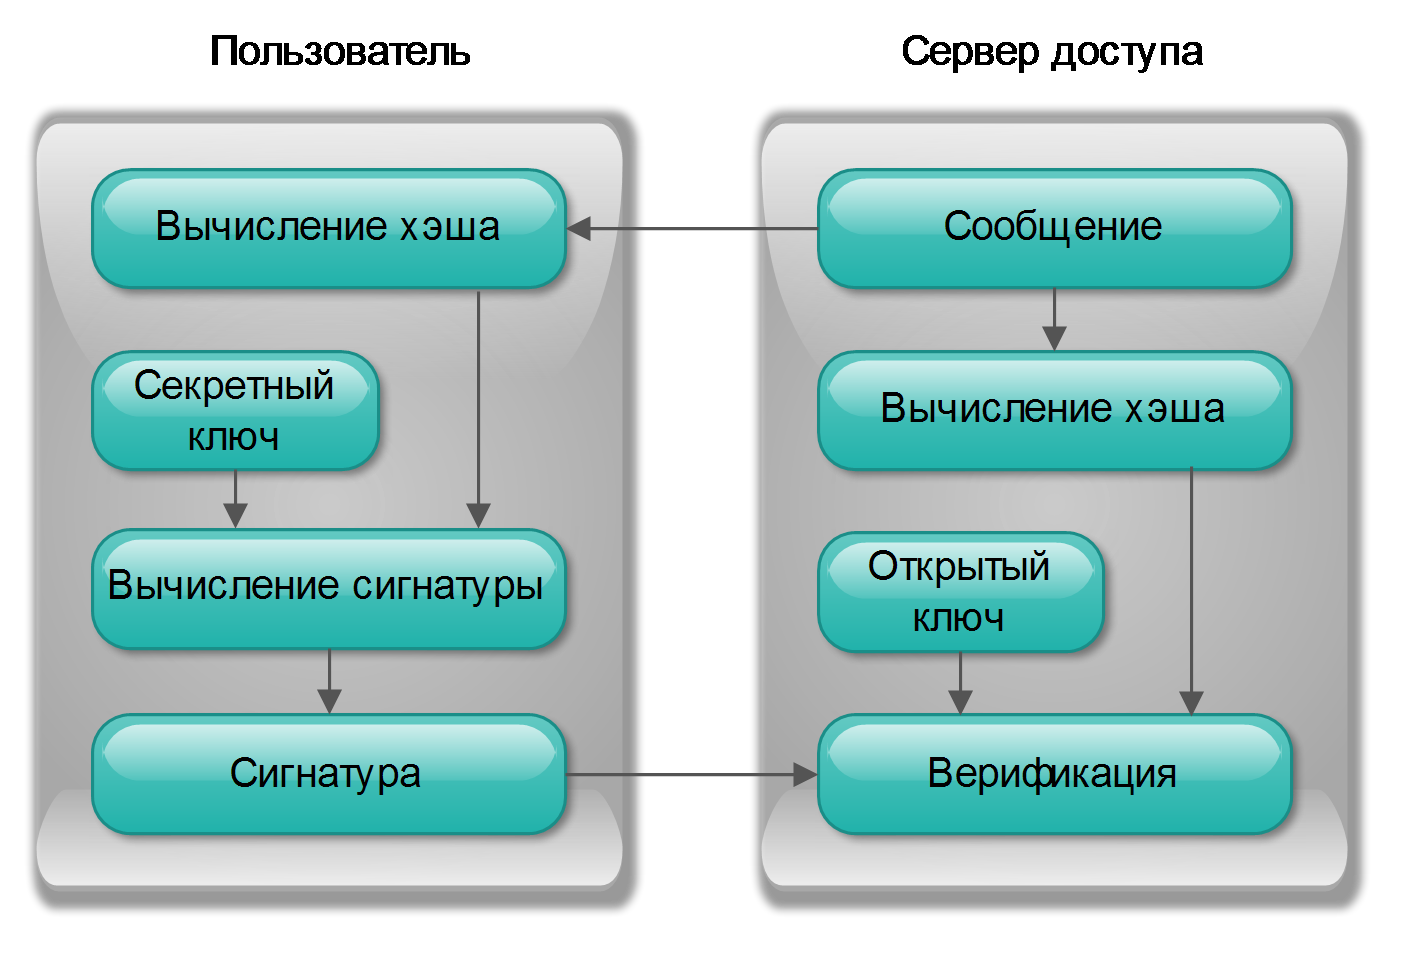
\includegraphics[width=1\linewidth]{3-1-1}}
\caption{Общая схема создания и верификации ЭЦП}
\label{ris:3.1.1}
\end{figure}

Процесс аутентификации на основе асимметричного алгоритма шифрования включает в
себя 3 макро-этапа:
\begin{itemize}
  \item Генерация ключей;
  \item Создание шифра к сообщению (документу);
  \item Верификация (проверка подлинности) самого сообщения и шифра.
\end{itemize}

Процесс генерации сопровождается заключением договора между удостоверяющим
центром и владельцем электронного ключа. Данный договор называется сертификатом и устанавливает
соответствие между открытым ключом и данными человека, однозначно
характеризующие его, и обладающего соответствующим ему (открытому ключу)
закрытым ключом. Потоки информационного обмена на данном этапе отражены на
рисунке~\ref{ris:3.1.2}.

\begin{figure}[h]
\center{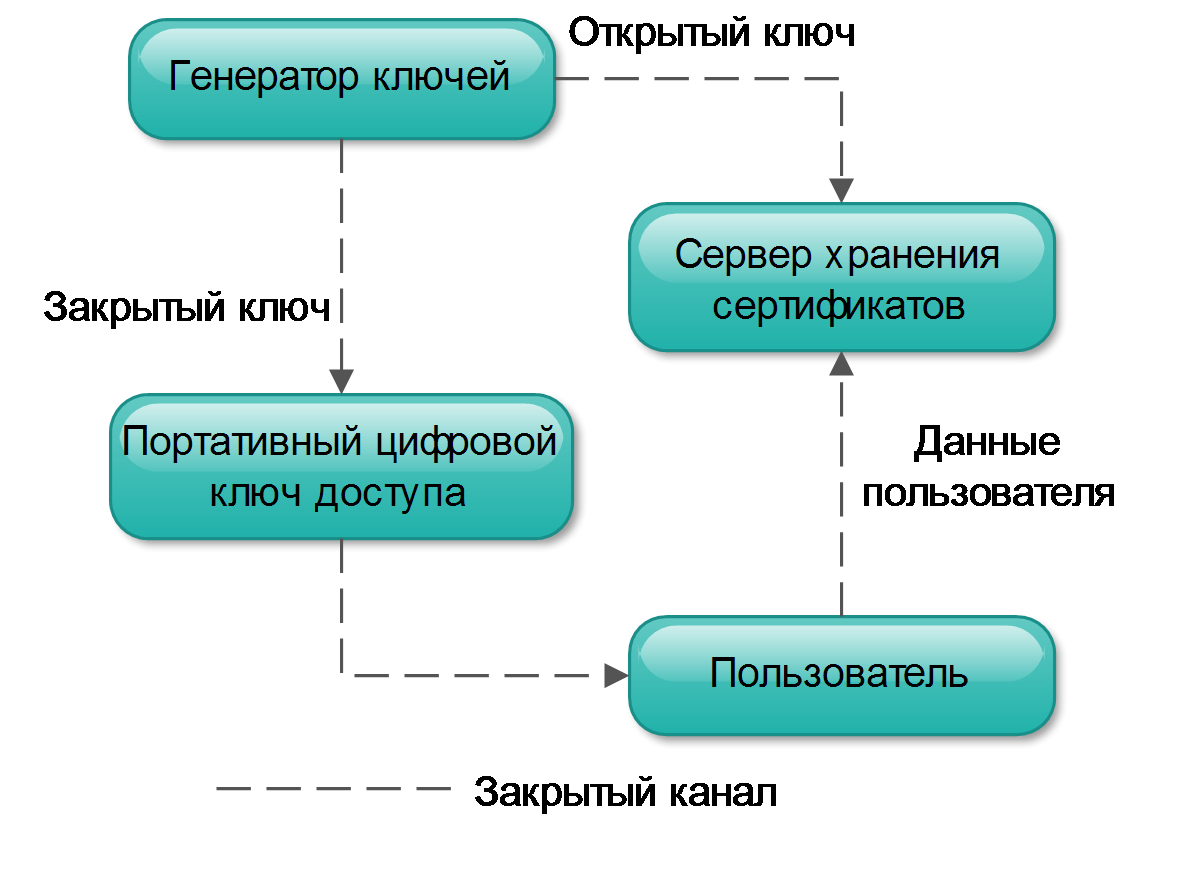
\includegraphics[width=1\linewidth]{3-1-2}}
\caption{Схема генерации индивидуального ключа}
\label{ris:3.1.2}
\end{figure}
  
Закрытый ключ является собственностью пользователя системы, их личным правом на
использование, имеющее юридическую силу, и не должен быть доступен другим людям
ни при каких обстоятельствах.  Поэтому цифровой носитель и алгоритм, осуществляющий генерацию
шифра, должен обеспечивать абсолютную секретность ключа и простейшие средства
безопасности, такие как:
\begin{itemize}
  \item полное скрытие ключа от визуального доступа на экране монитора при его
использовании;
  \item защита от нежелательной утраты цифрового носителя ключа,
вследствие чего он может стать доступен третьим лицам;
  \item защита от вредоносных
или шпионских программ, действующих неумышленно или целенаправленно на
компьютере, с которым работает пользователь в данный момент, для получения права
подписи от имени законного владельца закрытого ключа.
\end{itemize}

Для обеспечения поставленных требований необходимо разработать специальное
аппаратное устройство, которое возьмет на себя часть функций по организации
процессов информационного обмена и обеспечит защиту ключа на необходимом уровне,
которую невозможно достичь средствами наиболее распространённых операционных систем.
Кроме того, отдельное устройство должно быть сильно независимо от ПК, имееть
свою собственную память, к которой невозможно получить физический доступ и
обладать ограниченным набором команд.~\cite{evstifiev}
 
Данное устройство должно обладать следующими особенностями:
\begin{itemize}
  \item компактность, переносимость и малая себестоимость
изготовления;
\item устройство должно соединяться с ПК по средствам стандартных и наиболее
распространённых коммуникационных интерфейсов, используя стандартные протоколы
передачи данных. Речь идёт об использовании последовательного интерфейса USB. 
Недопустимо использовать интерфейсы, требующие дополнительного оборудования для
считывания данных с носителя ключа и не входящие в комплект стандартных
коммуникационных интерфейсов ПК, так как это снижает эффективность использования
данной технологии;
\item данное устройство должно иметь вычислительный механизм,
обладающий возможностью за относительно короткое время сгенерировать цифровую
подпись на основе закрытого ключа, <<спрятанного>> в памяти данного
устройства;
\item устройство-носитель закрытого ключа должно предоставлять единственный
интерфейс для установления связи только для определённого формата входных и
выходных данных, таким образом быть защищено от любого считывания данных из
памяти. На вход устройства подаётся сообщение в битовом виде. На выходе
получается сигнатура, которая имеет право быть
открытой и находиться в свободном обращении.
\end{itemize}  

Процесс вычисления сигнатуры (шифра) довольно сложный и выполняется в несколько
этапов, каждый из которых сопровождается информационным обменом различного рода.
Основной обмен информацией происходит между клиентской программой
(browser) и сервером доступа. Схема взаимодействий представлена на рисунке
~\ref{ris:3.1.3}.

\begin{figure}[h!]
\center{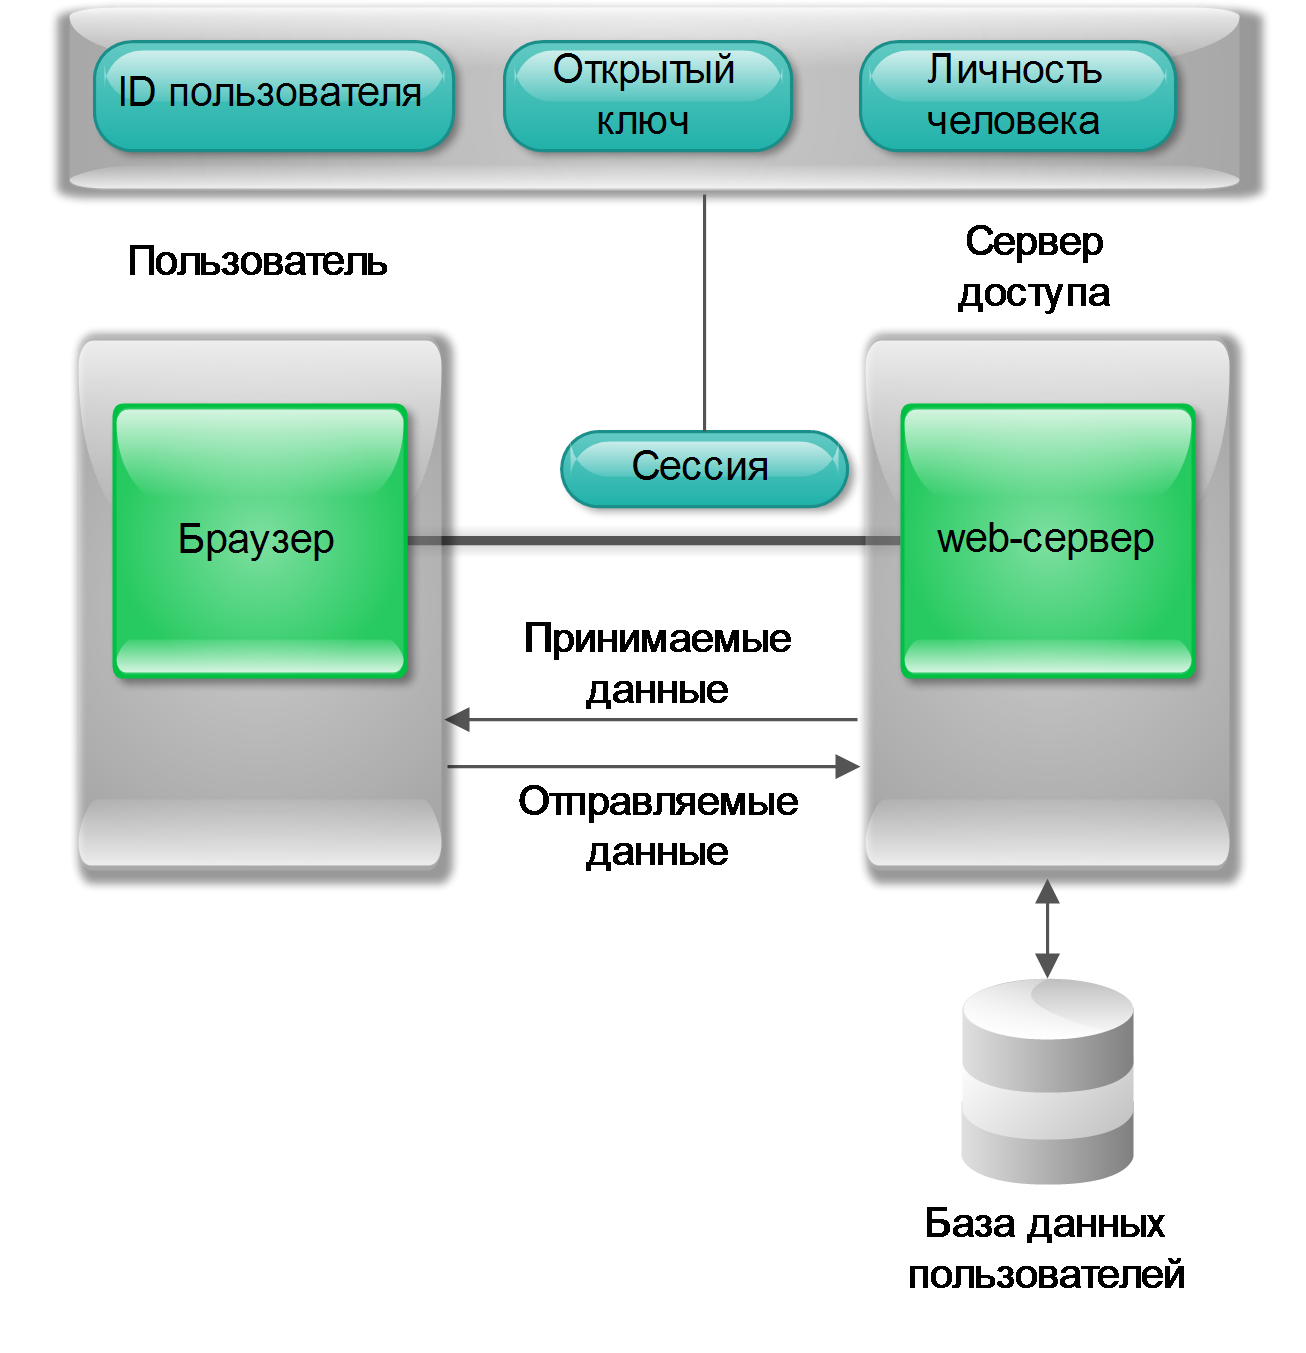
\includegraphics[width=1\linewidth]{3-1-3}}
\caption{Схема взаимодействия пользователя с сервером доступа}
\label{ris:3.1.3}
\end{figure} 
 
Пользователь через web-браузер соединяется с сервером доступа, и,
проходя аутентификацию, устанавливается сессия, в случае успешной проверки
подлинности пользователя. Возникает соответствие между идентификатором
пользователя в сети, личностью человека и его открытым ключом при
соответствующем обращении к базе данных.

В процессе аутентификации пользователю передаются данные в виде пакета
(получаемые данные) следующего содержания:
\begin{itemize}
  \item случайная последовательность (по другому ее называют <<соль>>);
  \item параметры алгоритма шифрования (они могут меняться с каждым разом);
  \item апплет – клиентская Web-программа, выступающая в роли согласующего звена
  между ПК и цифровым носителем закрытого ключа.
\end{itemize}

После проведения процедуры вычисления сигнатуры (шифра) на сервер отправляются
ответные данные включающие:
\begin{itemize}
  \item идентификатор пользователя в системе;
  \item сигнатура.
\end{itemize}

Полученная на сервере сигнатура закрепляется за конкретным пользователем,
определенным по его идентификатору, в рамках даннного сеанса. По данному
пользователю выбирается информация, необходимая для алгоритма проверки
подлинности сигнатуры (эта информация должна целиком существовать на сервере на
текущий момент), и осуществляется процедура верификации, в результате которой на
выходе получается положительный ответ, фиксируемый в базе данных в виде
создания сессии для пользователя, а так же в браузере клиента в виде
специального идентификатора сессии, задействовав технологию <<cookie>>.
В случае отрицательного ответа, от пользователя требуется проведение процедуры повторно, так как, вероятнее всего,
произошла подмена.

\begin{figure}[h!]
\center{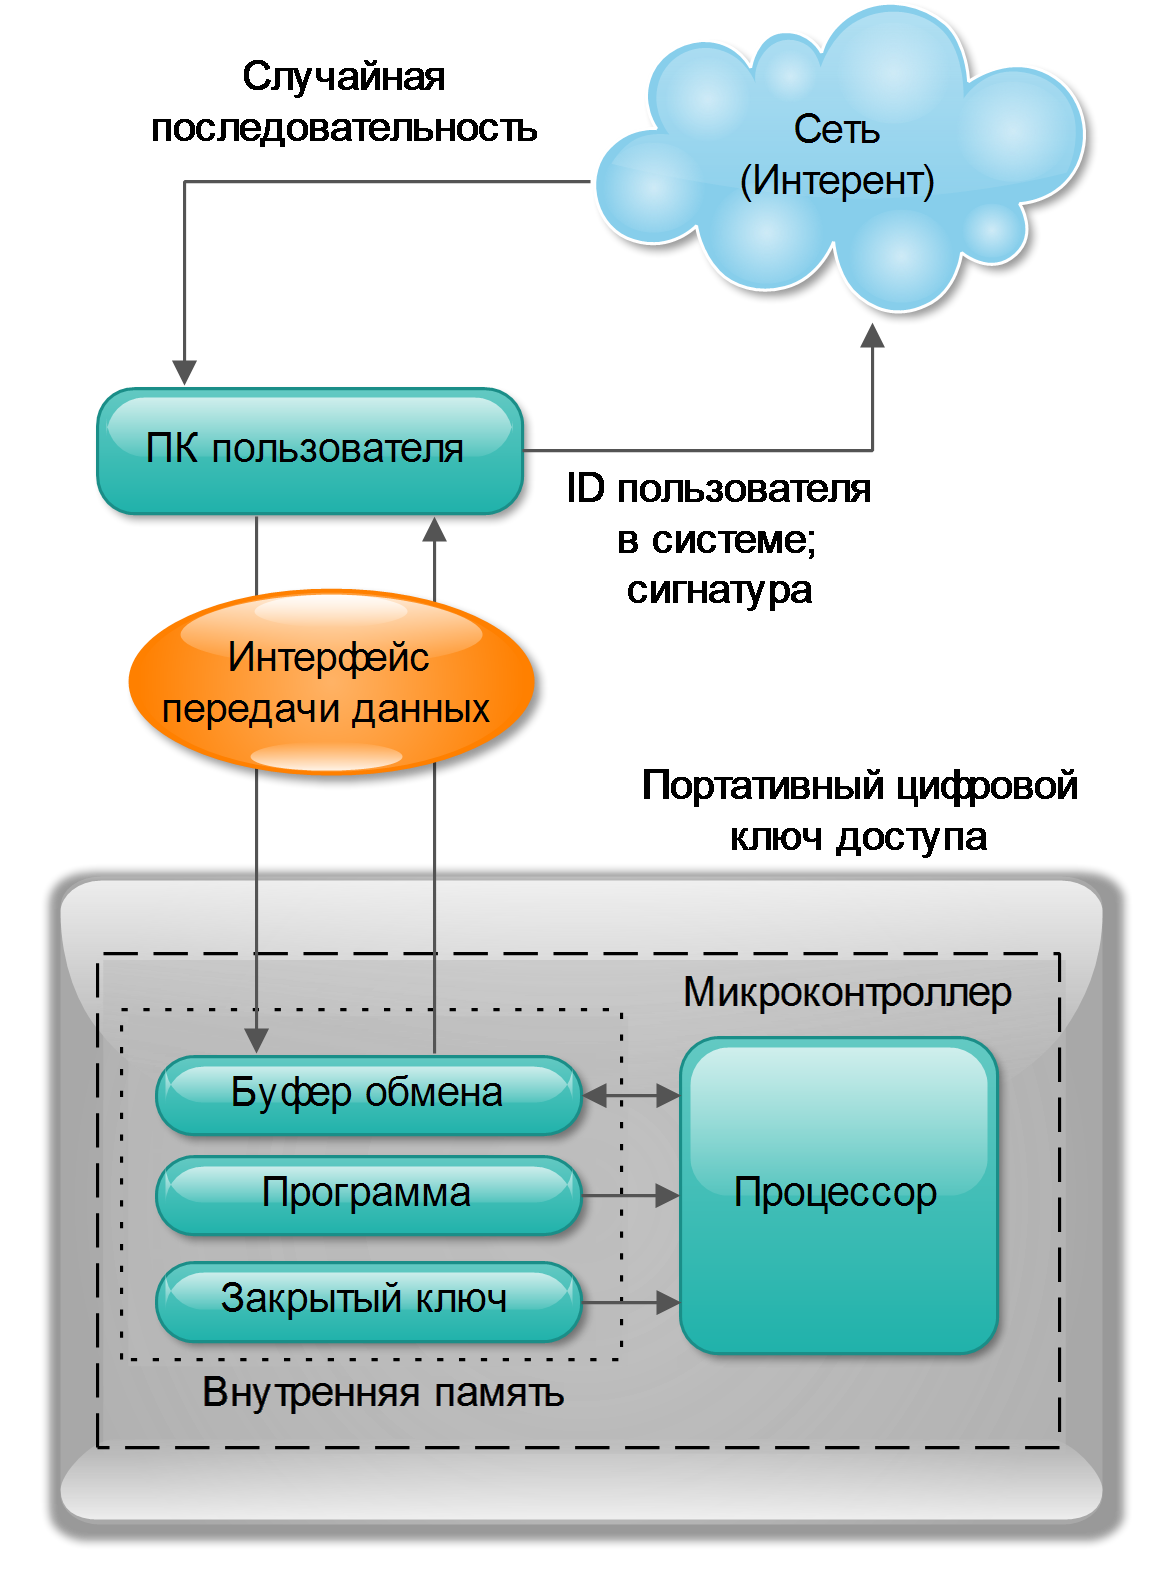
\includegraphics[width=0.6\linewidth]{3-1-4}}
\caption{Схема информационного обмена клиенской подсистемы в процессе
аутентификации}
\label{ris:3.1.4}
\end{figure} 

Схему, изображенную на рисунке~\ref{ris:3.1.3} можно детализировать с точки
зрения процессов, происходящих на стороне пользователя. Особую роль здесь играет
<<Портативный Цифровой Ключ Доступа>> (далее ПЦКД). Схема информационного обмена
клиенской подсистемы представлена на рисунке~\ref{ris:3.1.4}.

После получения пакета данных от сервера клиентская программа выполняет следующий ряд действий:
\begin{itemize}
  \item программа апплет устанавливает виртуальное соединение с носителем закрытого
ключа и получает ответ от согласующей программы, установленной на данном
носителе, об успешном подключении;
\item апплет запрашивает у пользователя короткий
код подтверждения, (PIN-код) тем самым дополнительно идентифицируя пользователя
как владельца данного носителя закрытого ключа. Данный код передаётся в
ПЦКД, который должен ответить положительным результатом. Система должны быть
оснащена защитой от взлома кода подбором;
\item апплет передает в ПЦКД случайную последовательность, полученную от
сервера доступа;
\item ПЦКД, получив на вход сообщение, вычисляет сигнатуру в соответствии с
алгоритмом, подгружая из памяти параметры алгоритма, идентификатор пользователя
в системе и закрытый ключ.
По окончании вычислений возвращает ответ на ПК;
\item апплет в свою очередь возвращает на сервер по открытому каналу полученные
данные, а так же идентификатор пользователя в системе.
\item финальным этапом является процедур верификации сигнатуры и установления
сессии.
\end{itemize}

Следует отметить что представленную технологию можно использовать как для
аутентификации пользователей, так и для проверки подлинности электронных
документов, не изменяя схему выполнения процесса, за исключением одного условия:
в качестве сообщения для выполнения алгоритмов будет выступать тело документа.

\section{Модель процессов}

Описание модели процессов предметной области было выполнено в нотации UML.
~\cite{uml_rambo,uml_rosenberg} <<Лицевой>> диаграммой процессов является диаграмма
вариантов использования (рисунок~\ref{ris:3.2.1}).

\begin{figure}[h!]
\center{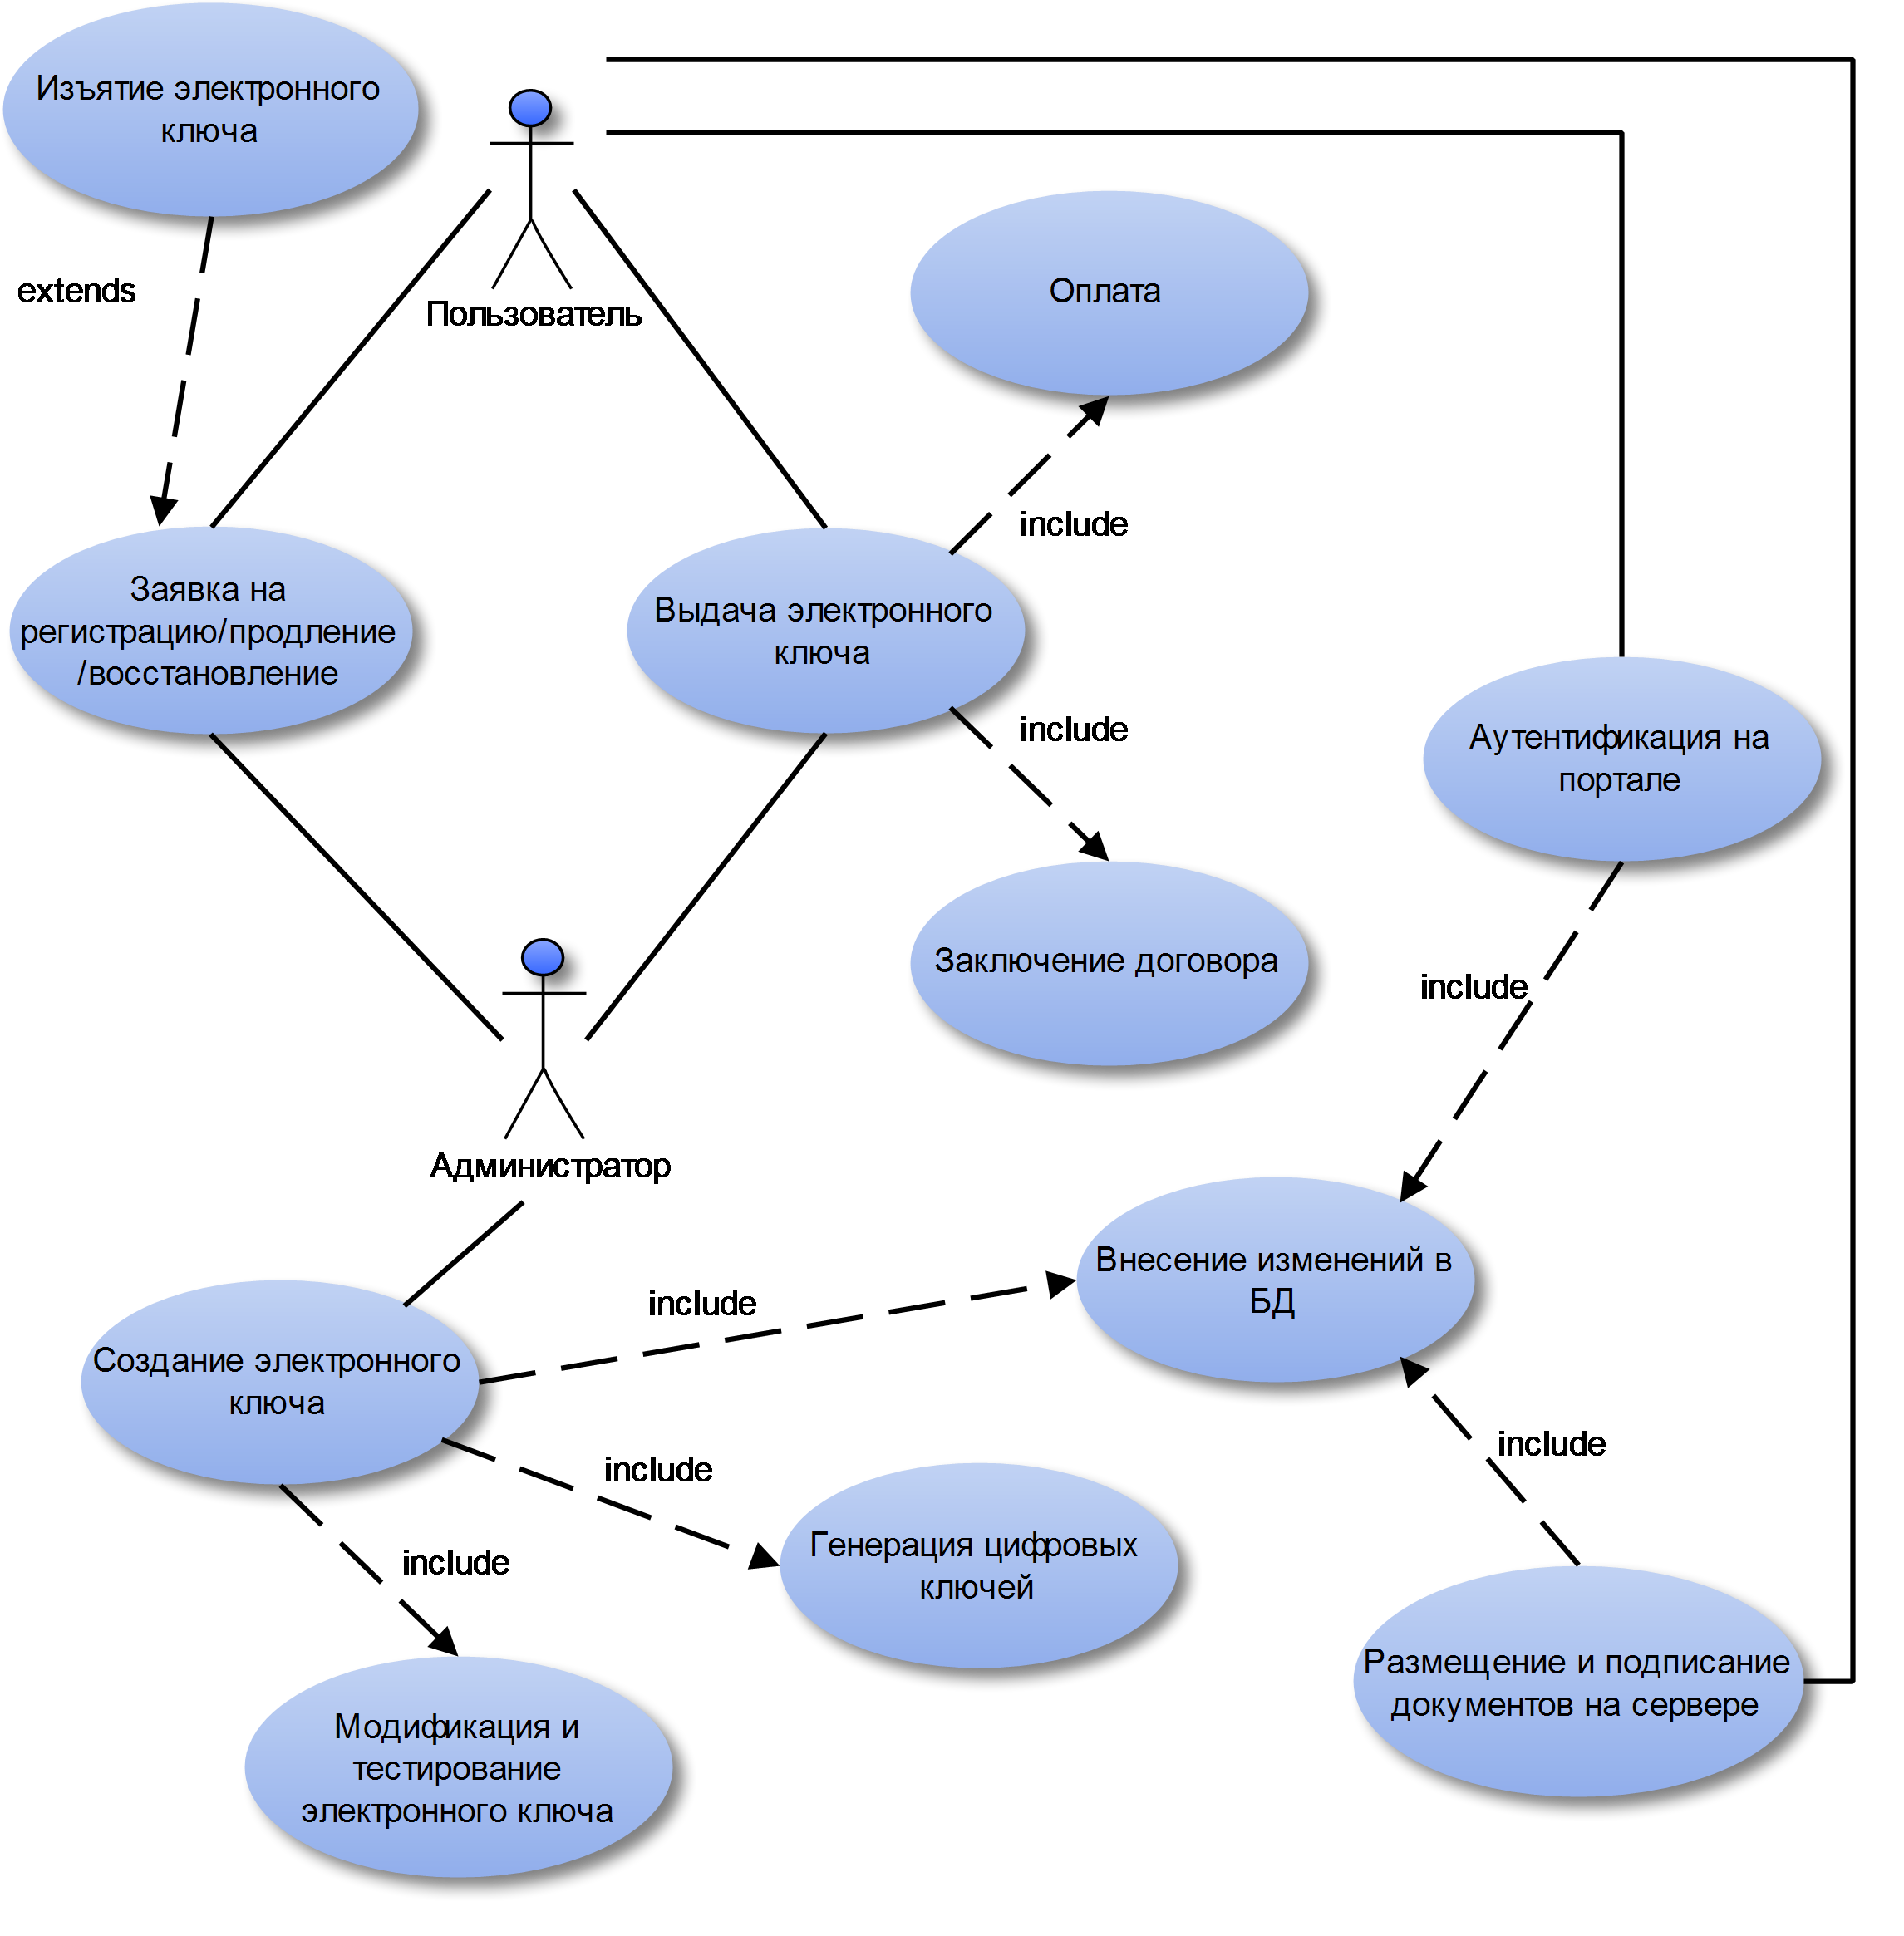
\includegraphics[width=1\linewidth]{3-2-1}}
\caption{Диаграмма вариантов использования}
\label{ris:3.2.1}
\end{figure} 

\begin{figure}[h!]
\center{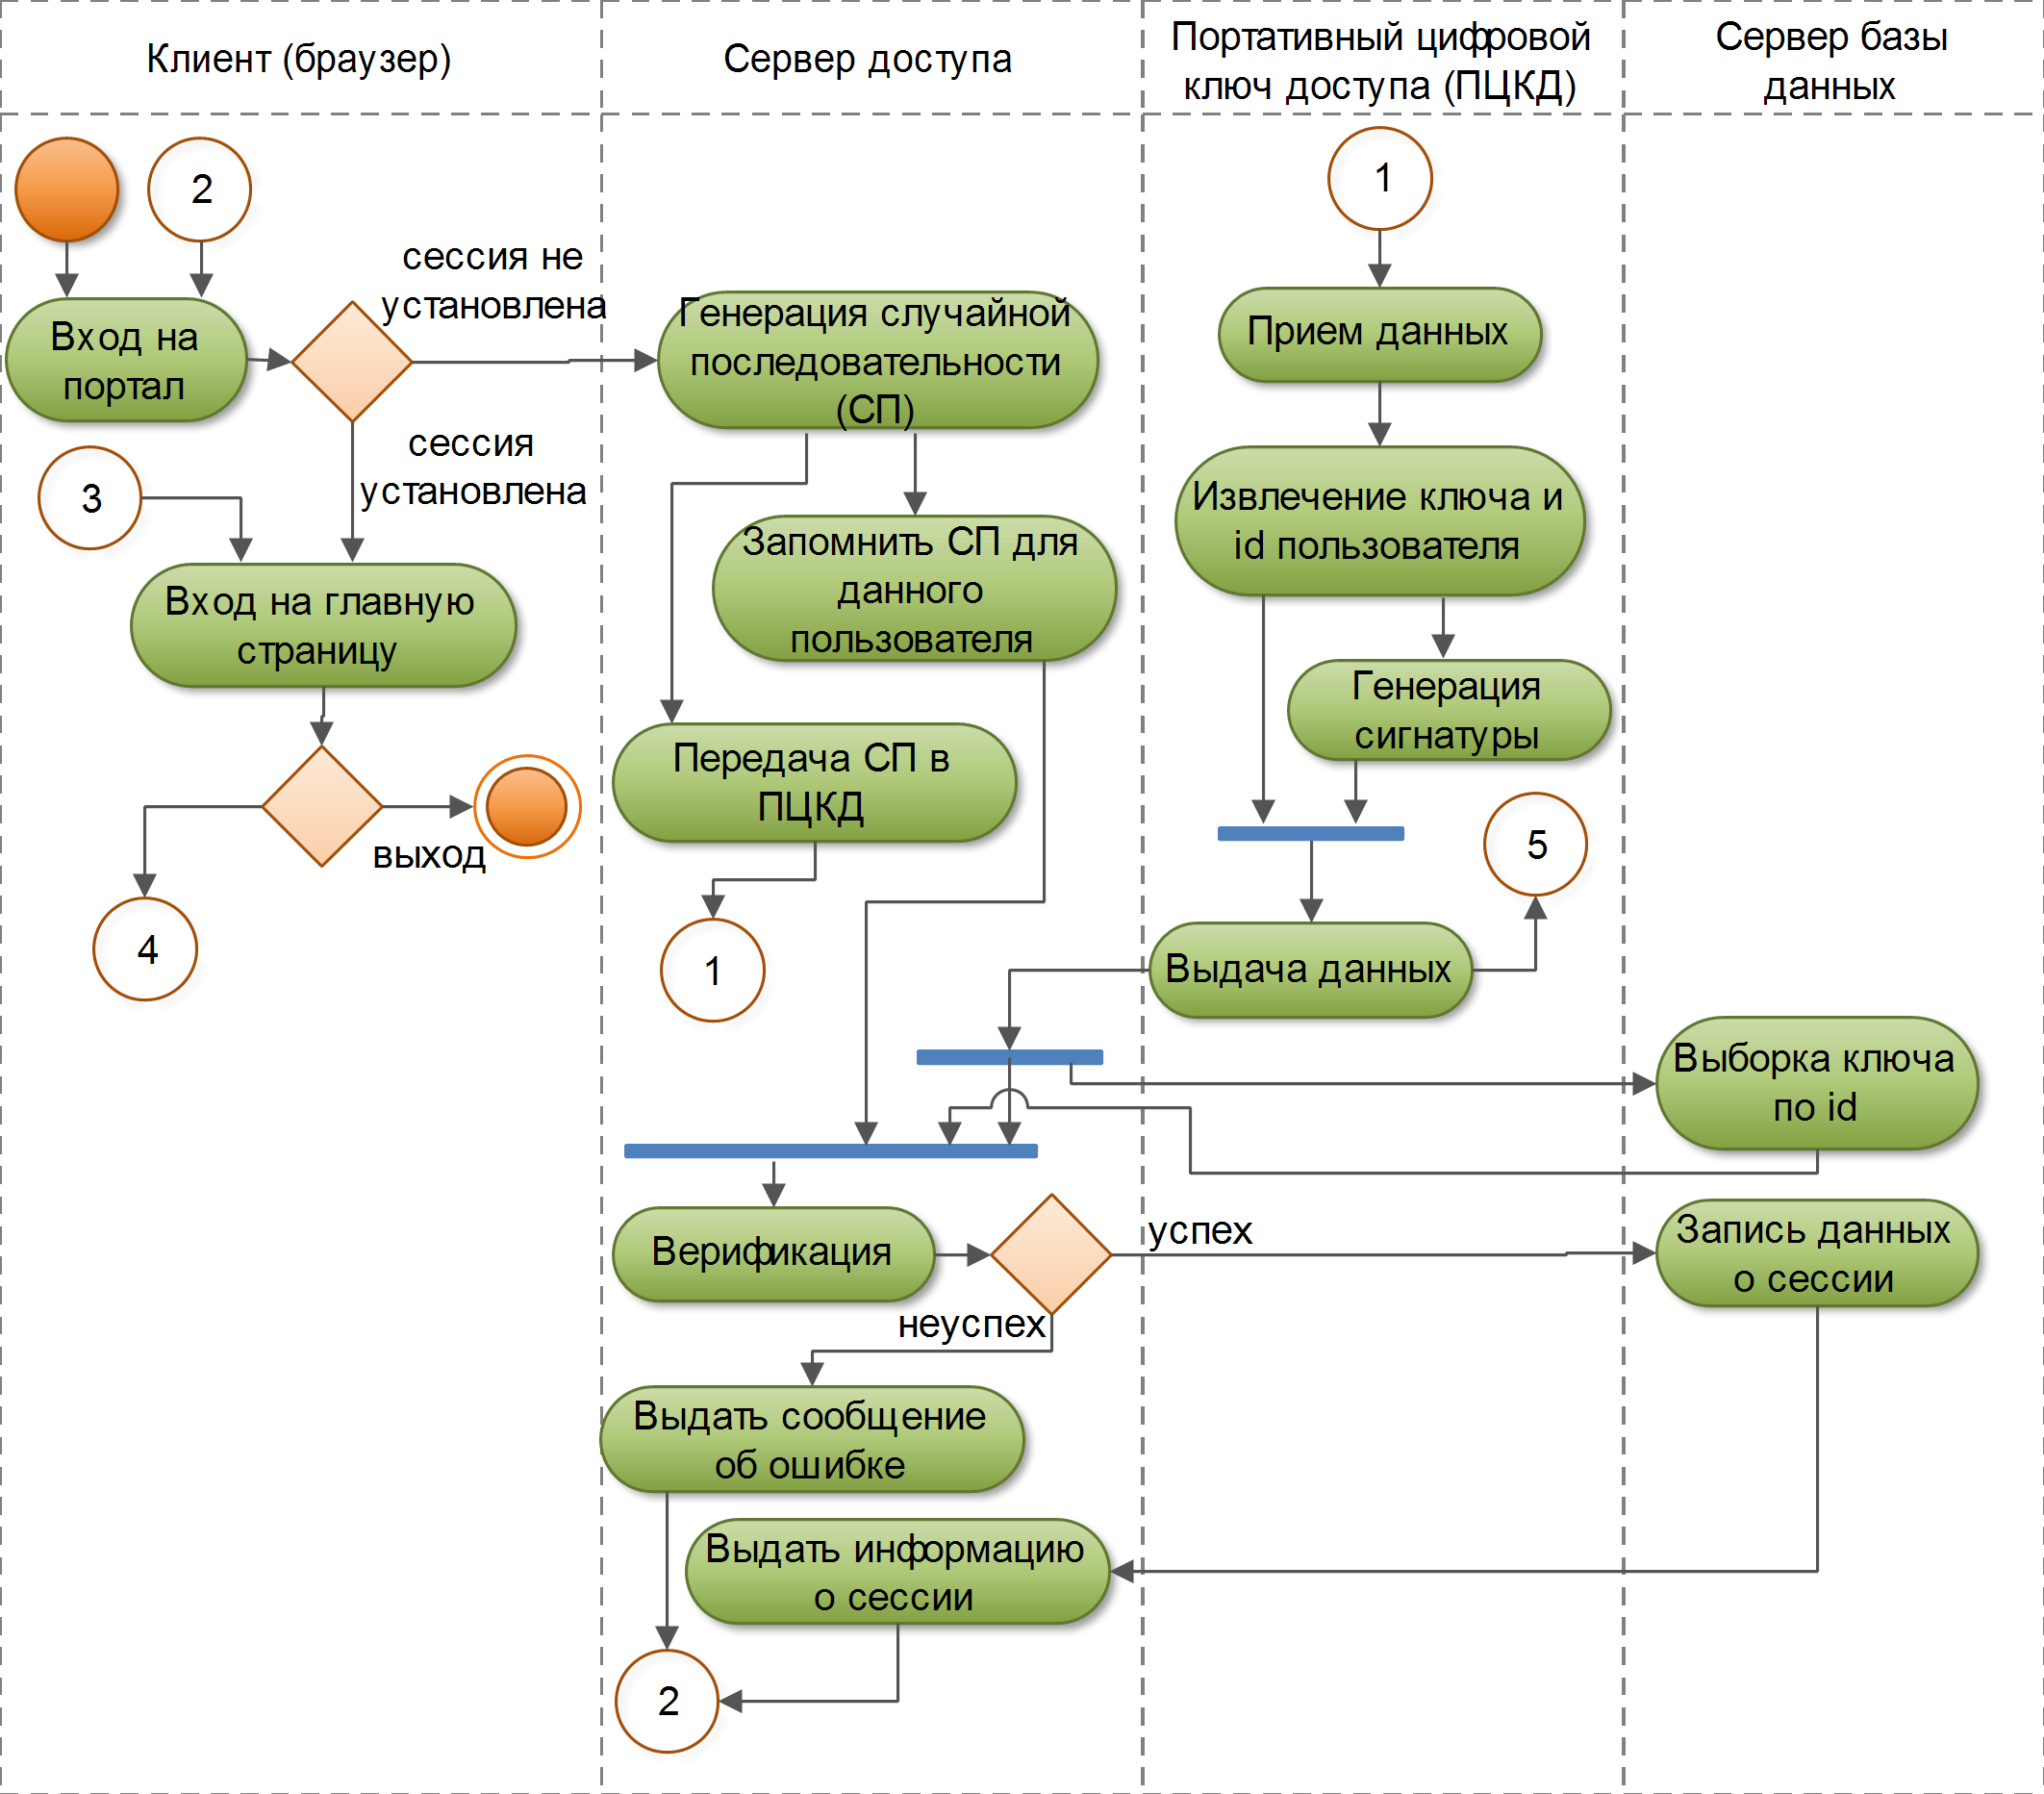
\includegraphics[width=1\linewidth]{3-2-2}}
\caption{Диаграмма активности (часть 1)}
\label{ris:3.2.2}
\end{figure} 

\begin{figure}[pH]
\center{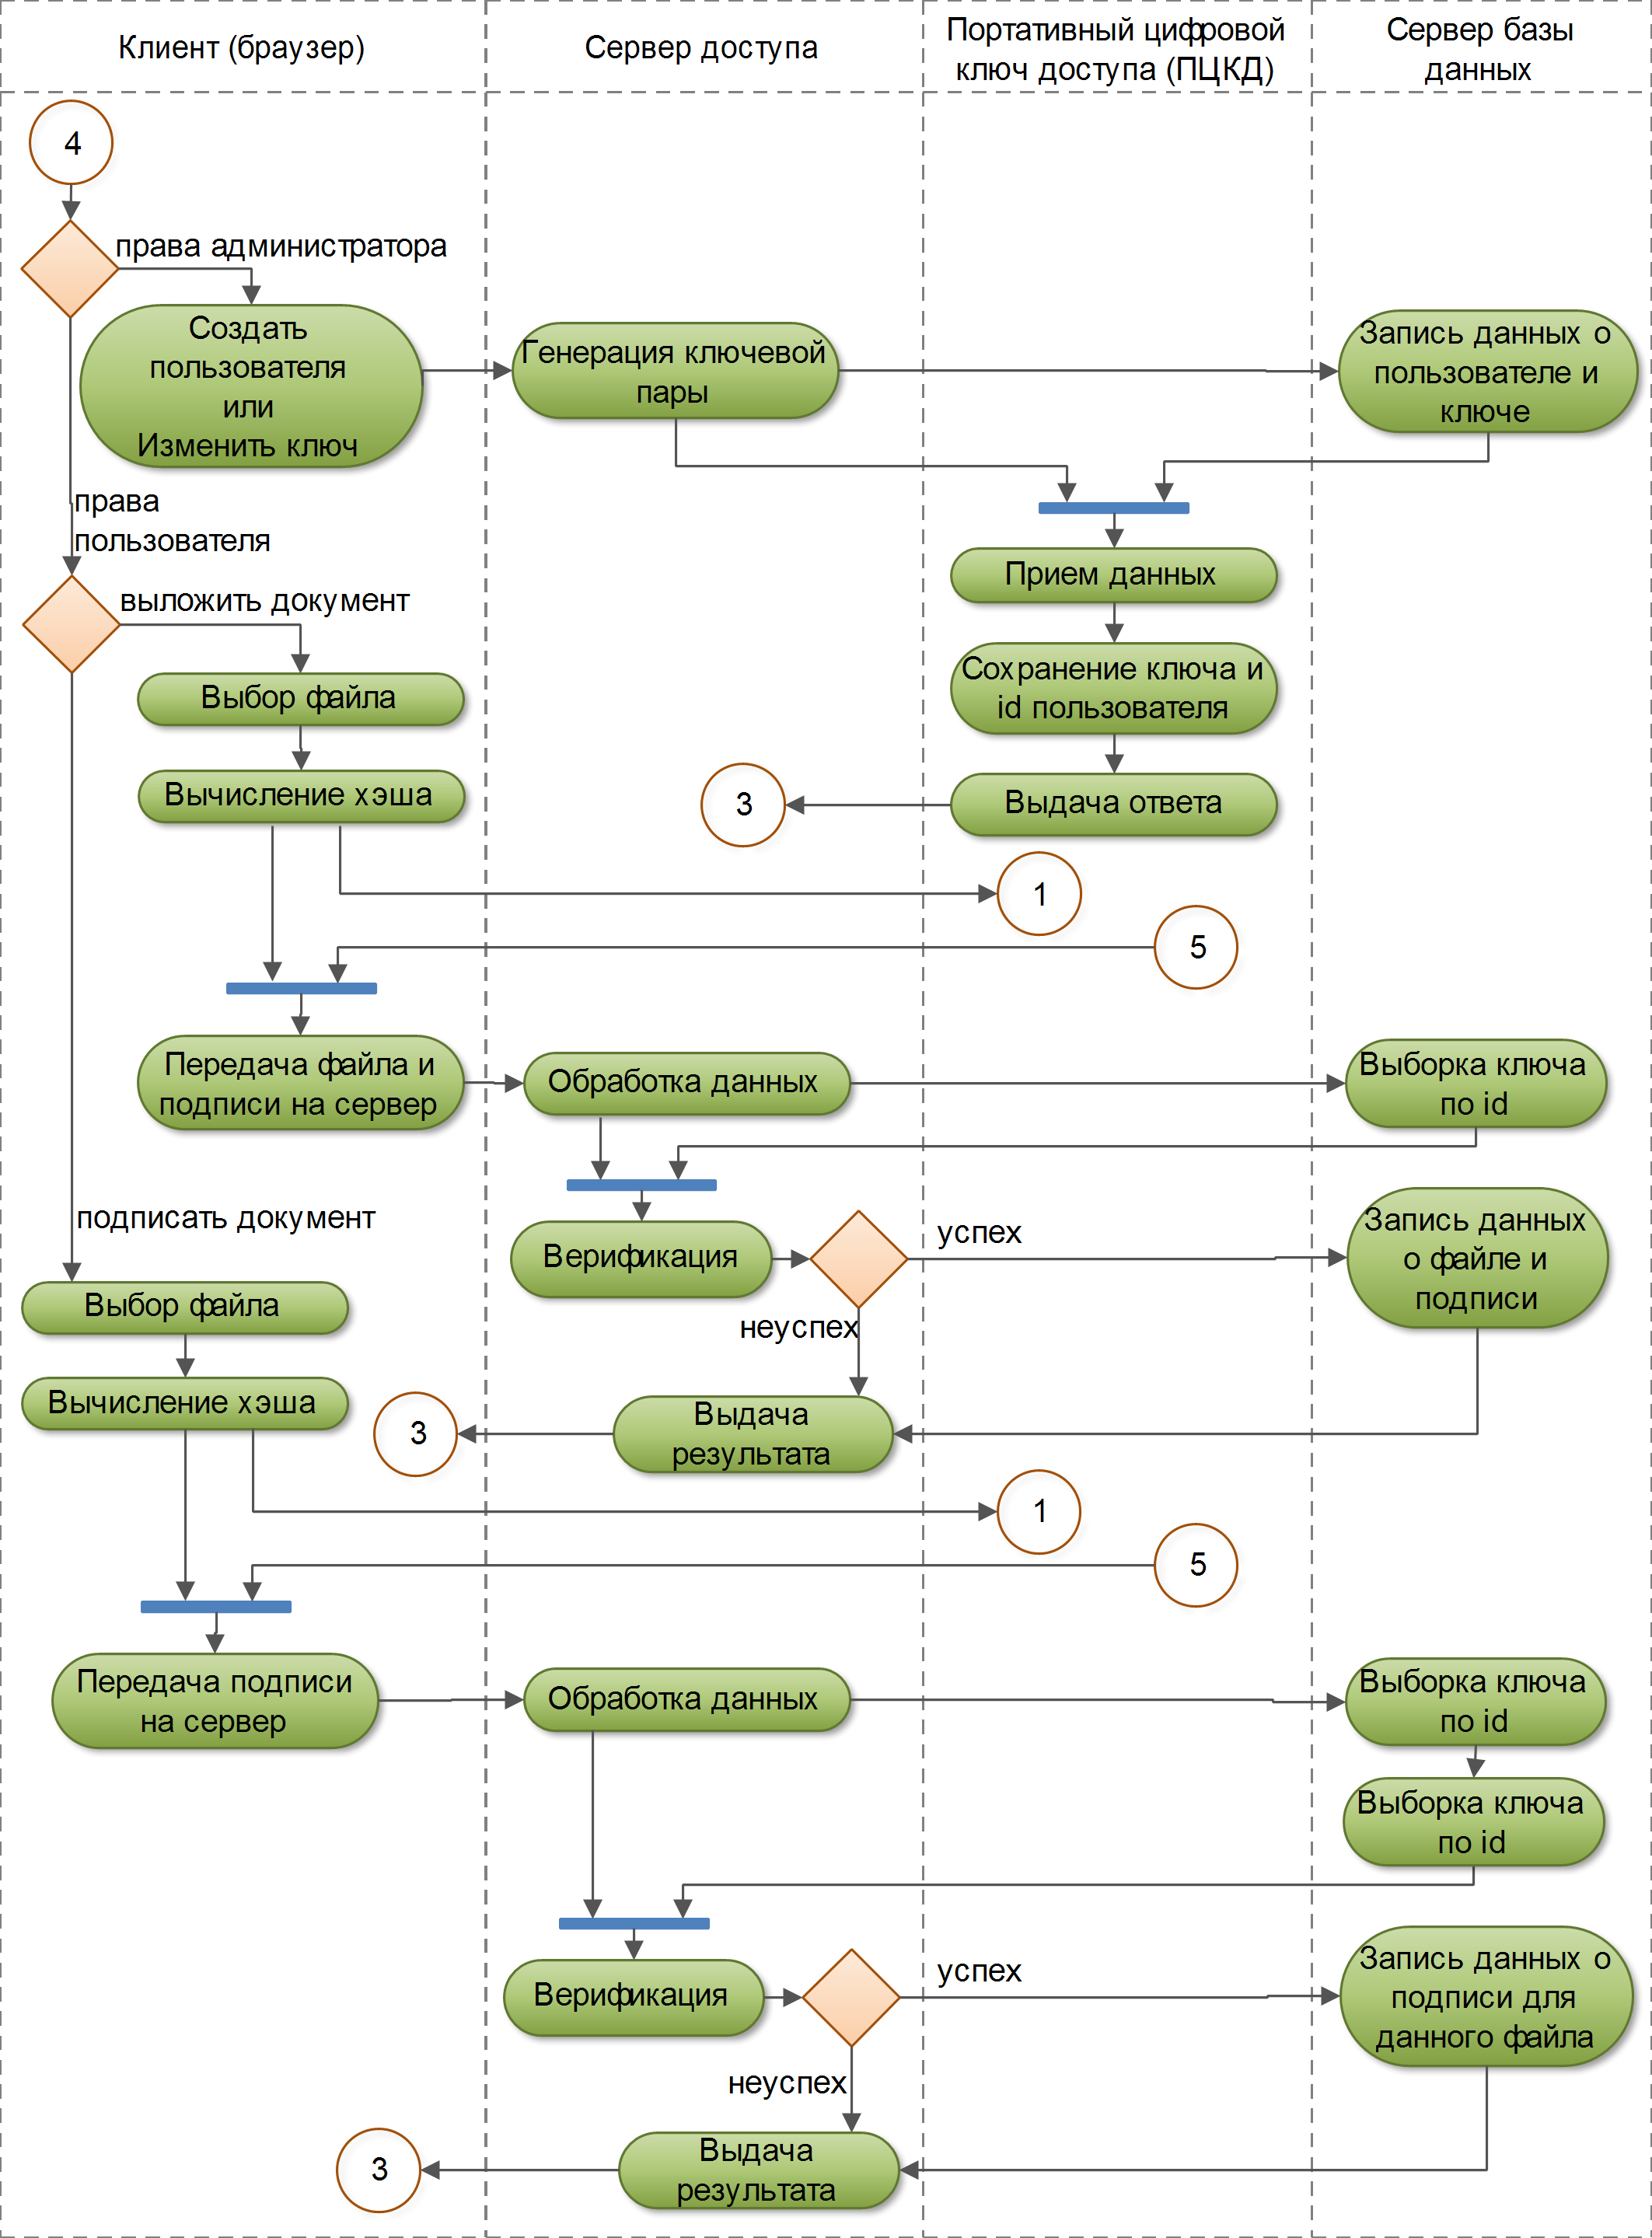
\includegraphics[width=1\linewidth]{3-2-3}}
\caption{Диаграмма активности (часть 2)}
\label{ris:3.2.3}
\end{figure} 

Основными функциональными действиями пользователя являются: аутентификация на
портале и размещение и подписание документов на сервере. Данные операции в
обязательном порядке вносят записи в базу данных.

Для осуществления данных функций, пользователю необходимо обладать портативным
цифровым ключем доступа (электронным ключем), который можно получить при
взаимодействии с администратором сервиса. Для этого необходимо подать заявку на
регистрацию/продление/восстановление электронного ключа, после чего ключ будет
выдан пользователю. В случае продления ключа старый ключ изымается у
пользователя. Выдача электронного ключа сопровождается заключением договора с
пользователем и оплатой.

Создание нового электронного ключа включает генерацию цифровых ключей, внесение
соответствующей информации в базу данных, а так же модификацию и тестирование
портативного цифрового устройства доступа.

Детализация диаграммы вариантов использования получила свое продолжение в виде
диаграммы активности (рисунок~\ref{ris:3.2.2} и рисунок~\ref{ris:3.2.3}).
Данная диаграмма наиболее точно и полно детализирует рассматриваемый процесс. 

\begin{figure}[h!]
\center{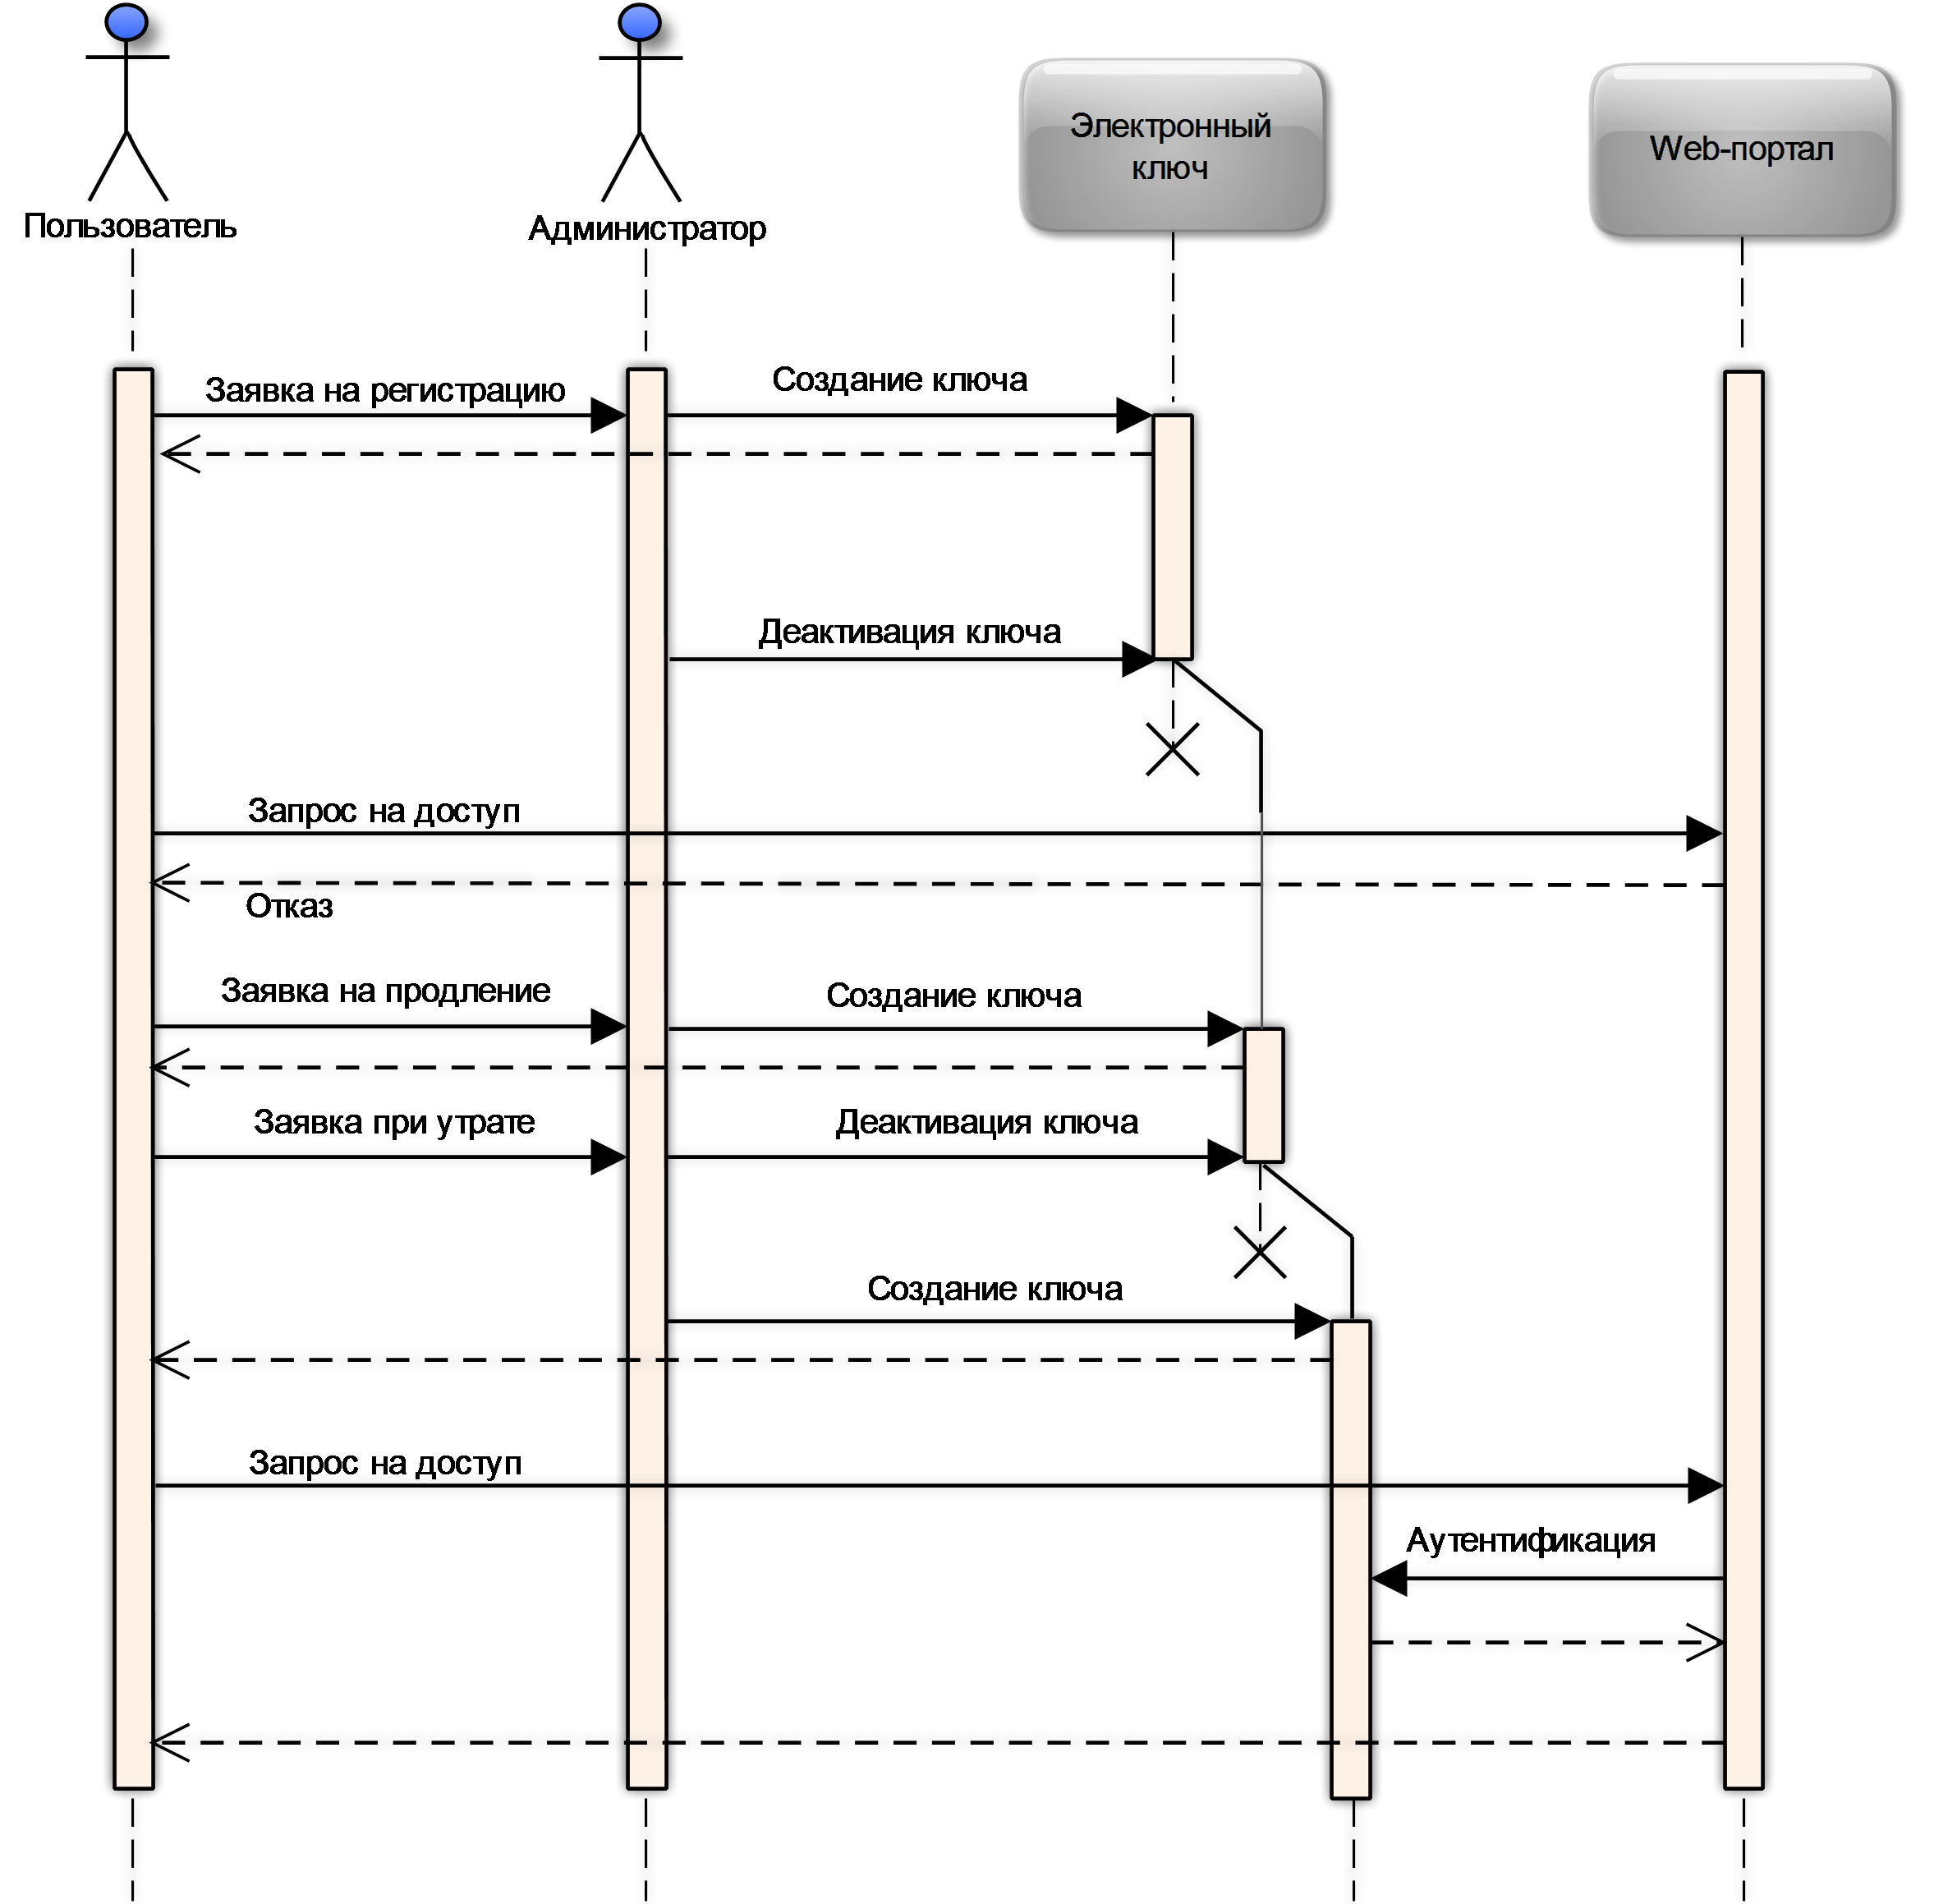
\includegraphics[width=1\linewidth]{3-2-4}}
\caption{Диаграмма взаимодействия}
\label{ris:3.2.4}
\end{figure} 

Диаграмма взаимодействия, фрагмент которой изображен на рисунке
~\ref{ris:3.2.4}, отображает линию жизни электронного ключа, а также действия
акторов в различных ситауциях.

Если пользователь еще не зарегистрирован в системе, то необходимо подать заявку
на регистрацию, после чего администратор создаст ключ, который будет передан
пользователю. По истечении установленного срока службы ключа произойдет
деактивация ключа и пользователь не сможет войти на портал с утратившим силу
ключом. В этом случае пользователь подает заявку на продление срока службы
ключа. При этом происходит изъятие устаревшего ключа, создание нового и выдача
обратно пользователю.

В случае утраты электронного ключа необходимо незамедлительно подать заявку
администратору, после чего ключ будет деактивирован и тут же создан новый. После
чего пользователь может получать доступ на портал в обычном режиме.
\section{Клиентская часть подсистемы аутентификации пользователей с применением
ПЦКД} 

В данной статье изложены технические аспекты и решения возможностей применения
портативных цифровых устройств для доступа в сети корпоративных порталов. В
частности, рассмотрены аппаратные особенности \textit{клиентской части} данной
системы доступа, как наиболее сложной с точки зрения организации, а также
сопутствующие программные средства и способы их интеграции для установления
взаимодействия между звеньями сложной цепочки компонентов системы.

\subsection{Технические особенности построения портативного цифрового устройства
доступа} 

В соответствии с предложенной методикой~\cite{concept_PCKD}, в качестве основной функции
ПЦКД выступает не только хранение идентификационных данных, но и непосредственное
участие в процессе генерации шифрограммы. Исходя из этого, следует, что
элементная база ПЦКД должна основываться на микропроцессорной системе, имеющей
аппаратный вычислитель.

В качестве ядра данной системы предлагается использовать 32-ух разрядный
микроконтроллер семейства AT91SAM7 от фирмы Atmel. Технические характеристики и
полный перечень особенностей приведен в таблицах описания для данного
микроконтроллера.~\cite{atmel}

Важно отметить следующие особенности данного микроконтроллера, которые
необходимы для решения всех аспектов поставленной задачи:
\begin{itemize}
  \item относительно малые размеры, позволяющие сделать устройство портативным;
  \item высокое быстродействие, применительно к возложенным функциям;
  \item невысокая стоимость, что позволит сделать продукт массовым;
  \item наличие порта устройства USB 2.0, позволяющего облегчить подключение к
  ПК;
  \item наличие  встроенных битов
блокировки и бита защиты, которые позволяют защитить прошивку микроконтроллера
от несанкционированной перезаписи или хищения, что немаловажно в задачах
криптографии.
\end{itemize}

При проектировании ПЦКД была разработана схема электрическая принципиальная
(см. Приложение~\ref{pril:A}, рисунок~\ref{ris:cxeme}), основа которой предложена на
официальном сайте разработчика микроконтроллера.~\cite{olimex}

\subsection{Протокол взаимодействия ПК и ПЦКД}

Немаловажной составляющей предложенной методики является выбор протокола для
информационного обмена между ПК и ПЦКД. Основными критериями для выбора
протокола являются:
\begin{itemize}
  \item возможность реализации протокола выбранным микроконтроллером;
  \item высокая
надежность и скорость передачи данных по интерфейсу;
\item возможность создания
коммуникации между ПК и ПЦКД, используя известные методы и подходы.
\end{itemize}

Исходя из поставленных требований, в качестве протокола для взаимодействия ПК и
ПЦКД был выбран протокол USB HID. HID-устройства (Human Interface Device) это
устройства взаимодействия компьютера и человека, такие как:
\begin{itemize}
  \item клавиатуры, мыши, джойстики и другие указатели;
  \item игровые
рулевое управление и педали;
\item кнопки, переключатели, регуляторы; 
\item различные датчики и считыватели;
 \item и т. п.
\end{itemize}

Принципиально на основе HID-технологии можно организовать взаимодействие с любым
устройством, даже если оно не является в строгом смысле интерфейсным устройством
человека и компьютера.

На стороне хоста обменом с устройством будет руководить стандартный
 HID-драйвер, включенный в поставку операционной системы.

Максимально возможная скорость передачи данных при такой организации обмена
составляет 64 Кбит/сек. Такой показатель в сравнении с 12 Мбит/сек полной
скорости USB-шины является большим минусом HID-технологии в вопросе выбора
конкретной USB-реализации. Однако, для поставленной задачи указанной скорости
вполне хватает. Беря во внимание размерности параметров алгоритмов шифрования,
максимальное количество данных, передаваемых по USB интерфейсу равна 4 Кбайт в
обоих направлениях, следовательно, для передачи данных потребуется менее 500 мс.

При разработке HID-устройства необходимо обеспечить следующие требования,
налагаемые спецификацией:
\begin{itemize}
  \item полноскоростное HID-устройство может передавать 64000 байт каждую секунду: по
64 байта каждые 1 мс; низкоскоростное HID-устройство имеет возможность передать
вплоть до 800 байт в секунду: по 8 байт каждые 10 мс;
\item HID-устройство может
назначить частоту своего опроса для определения того, есть ли у него свежие
данные для передачи;
\item обмен данными с HID-устройством осуществляется
посредством специальной структуры, называемой репортом (Report). Каждый
определенный репорт может содержать до 65535 байт данных. Структура репорта
имеет весьма гибкую организацию, позволяющую описать любой формат передачи
данных. Для того, чтобы конкретный формат репорта стал известен хосту,
микроконтроллер должен содержать специальное описание – дескриптор репорта;
\end{itemize}

HID-устройства должны иметь конечную точку
типа Interrupt IN и могут иметь конечную точку типа Interrupt OUT. С помощью них
устройство может выдавать данные хосту и получать их от него. Типы и направления
передач мы рассматривали в статье, посвященной основам организации USB-шины.
Обмен данными с HID-устройствами осуществляется при помощи репортов. Они бывают
двух типов:
\begin{itemize}
  \item INPUT- и OUTPUT-репорты используются для периодических передачи и приема
данных;
\item FEATURE-репорты обычно используются для установки различных
параметров и свойств, а также передачи других данных в тех случаях, когда
предположить периодичность появляния таких данных сложно. FEATURE-репорты бывают как
направления IN, так и направления OUT. Такие репорты передаются и принимаются
только по каналу нулевой конечной точки.
\end{itemize}

При идентификации HID-устройств хост определяет, что устройство относится к HID
классу по коду класса 0x03 в дескрипторе интерфейса. Кроме того, HID-устройства
имеют специальные дескрипторы. После того как хост определит, что устройство
принадлежит к HID классу, он передает управление устройством соответствующему
драйверу и обмен  ведется под его руководством.~\cite{kozlov}

Следуя данной спецификации интерфейса была предложена схема организации
программных компонентов для обеспечения информационного обмена между ПК и ПЦКД,
показанная на рисунке~\ref{ris:3.3.1}.

\begin{figure}[h!]
\center{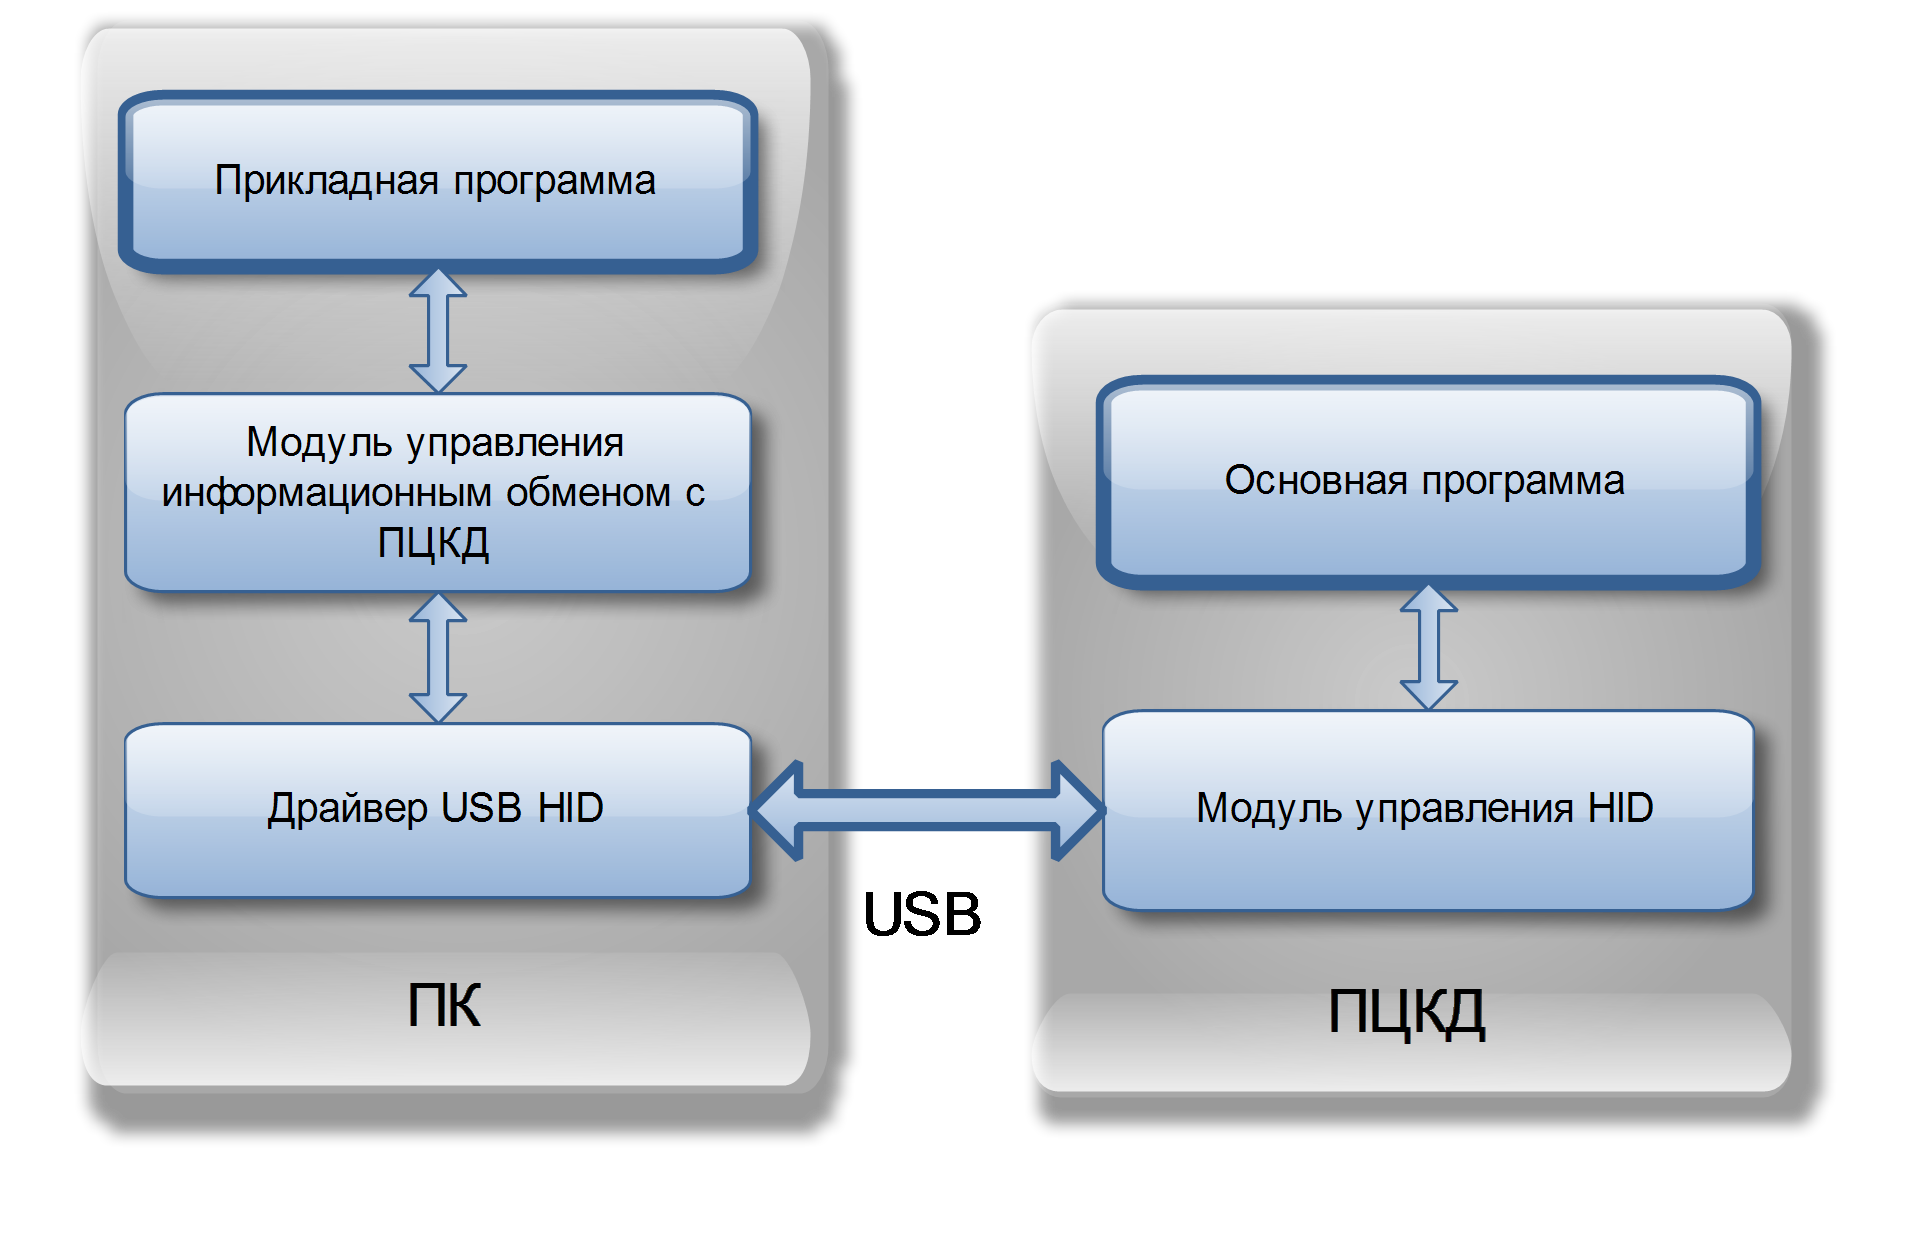
\includegraphics[width=1\linewidth]{3-3-1}}
\caption{Схема организации программных компонентов, обеспечивающих передачу
данных между ПК и ПЦКД с помощью USB HID}
\label{ris:3.3.1}
\end{figure}
 
На схеме представлены две основных программы, выполняющие целевую функцию и
взаимодействующие между собой: для ПК -- \textit{Прикладная программа}, для ПЦКД
-- \textit{Основная программа}. Остальные компоненты необходимы для
осуществления взаимодействия устройств через HID интерфейс. Модули управления
имеют набор функций, которые предназначены для приёма/передачи сообщений.

\subsection{Подходы к организации доступа к локальным ресурсам ПК из браузера}

Исходя из поставленной задачи, доступ к серверу должен осуществляться по
протоколу HTTP/HTTPS для максимального облегчения в использовании, а,
следовательно, все процессы по аутентификации пользователя на web-портале должны
быть инициированы браузером, выполняться в его рабочем пространстве и
контролироваться им. Согласно предложенной методике, часть действий, необходимых
для аутентификации, должны выполняться ресурсами ПЦКД. Возникает ситуация, при
которой необходимо создать механизм двустороннего взаимодействия с ПЦКД
средствами интернет-технологий, которые позволяют выполнять сценарии на стороне
клиента. Таким образом, схема организации программных компонентов
(рисунок~\ref{ris:3.3.1}) получает новую интерпретацию, где в роли прикладной
программы выступает браузер или сценарий, работающий под его управлением –
web-сценарий (рисунок~\ref{ris:3.3.2}).

\begin{figure}[h!]
\center{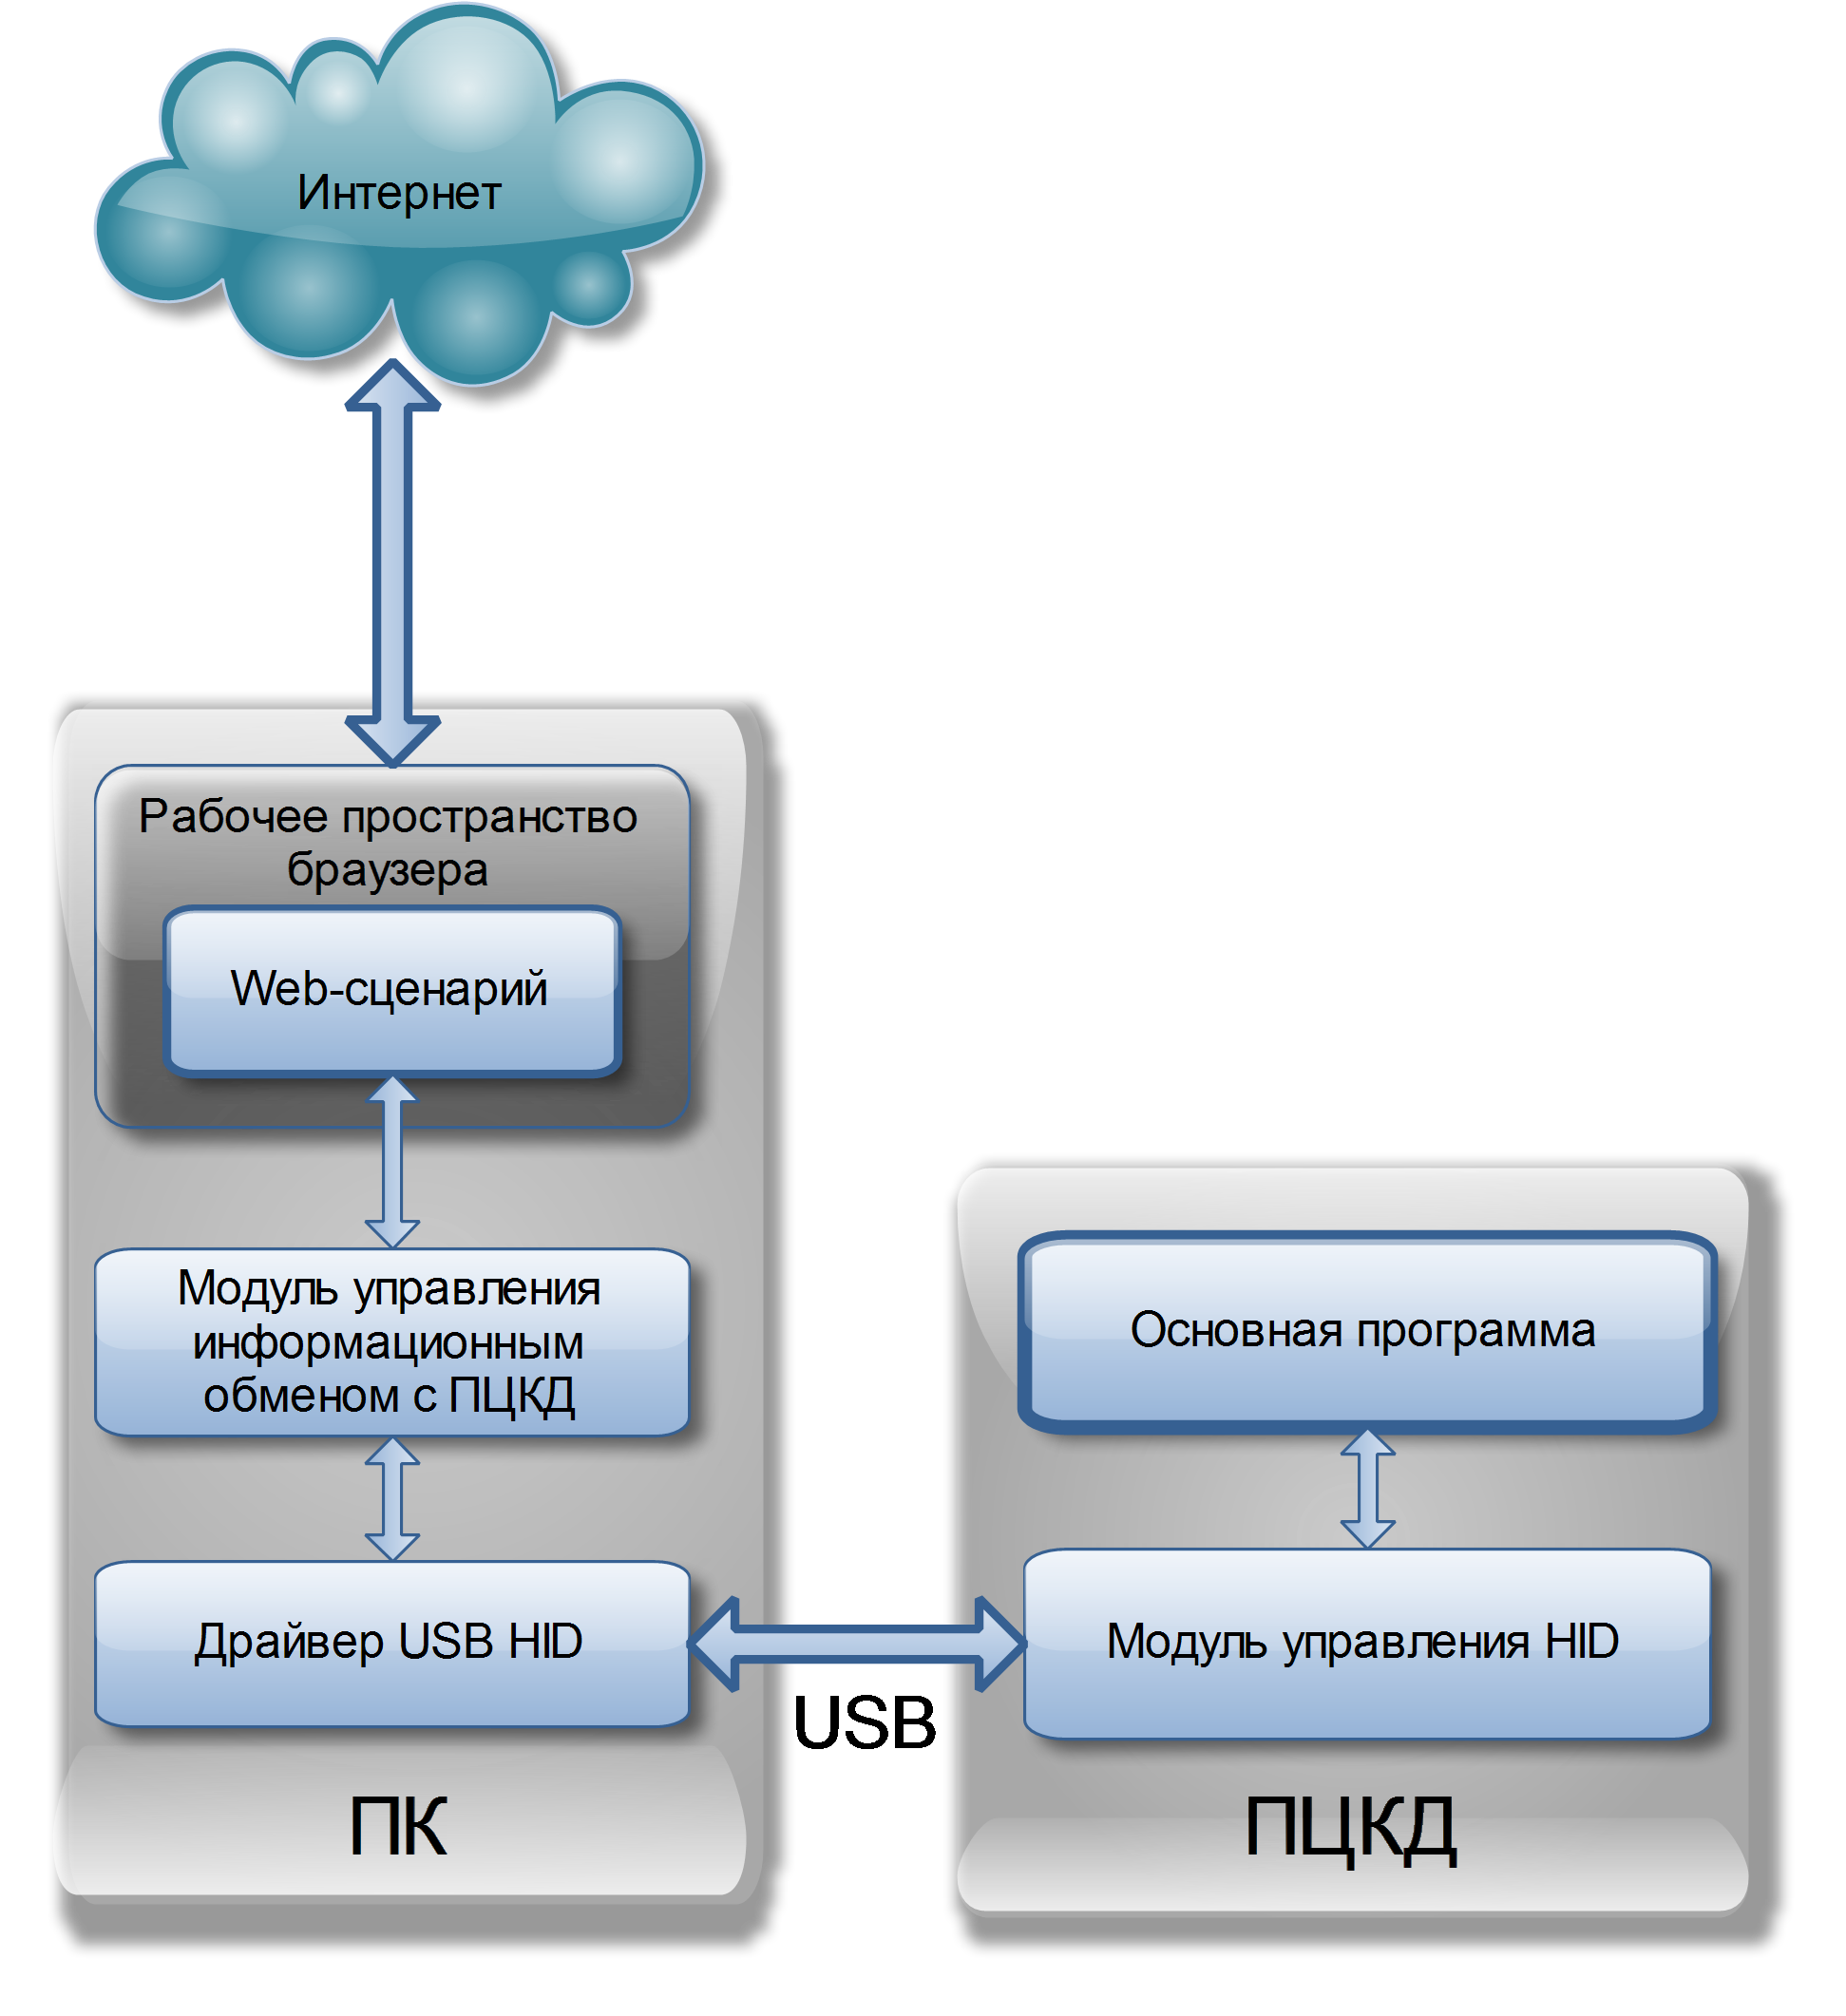
\includegraphics[width=1\linewidth]{3-3-2}}
\caption{Схема организации программных компонентов обеспечивающих передачу
данных между ПК и ПЦКД через браузер}
\label{ris:3.3.2}
\end{figure}

Данная схема весьма затруднительна с точки зрения её реализации, поскольку
возникает противоречие. С одной стороны, в соответствии с данной схемой,
взаимодействие с ПЦКД необходимо производить через драйвер ОС, относящийся к
локальным ресурсам ПК и являющийся внешним окружением по отношению к браузеру. С
другой стороны, браузер является средством доступа в глобальную сеть и имеет
мощные средства защиты от несанкционированного доступа к локальным ресурсам ПК,
и пресекает любые попытки обращения к ним.

Таким образом, возникает проблема, при которой необходимо получить доступ к
локальным ресурсам средствами браузера, что не позволяет делать его политика
безопасности.

Решение данной проблемы может получить развитие в следующих направлениях:
\begin{itemize}
  \item Создание модуля для браузера (плагина);
  \item Создание Java-апплета;
  \item Создание прикладной программы для ОС, которая будет работать независимо
  и выступать в роли посредника между web-сценарием и модулем взаимодействия с
  ПЦКД.
\end{itemize}

При анализе данных подходов были выявлены достоинства и недостатки каждого из
них в контексте проблемы, описанной выше. Полученные результаты зафиксированы в
таблице~\ref{tab:1}.

\begin{table}[ht]
  \small
  \centering
  \begin{tabular}{|p{3cm}|p{6cm}|p{7cm}|}
    \hline
	\textbf{Название технологии} & \textbf{Преимущества} & \textbf{Недостатки} \\
	\hline 
	\textit{Плагин для браузера} & полная интеграция с ОС на низком уровне, что
	упрощает механизм взаимодействия с ПЦКД & неудобство в использовании:
	\begin{itemize}
	  \item необходимость в отдельной установке;
	  \item для каждой версии браузера -- свой плагин.
	\end{itemize}  \\ \hline
	\textit{Java-апплет} & полная совместимость со всеми браузерами & получение
	доступа к локальным ресурсам возможно только после доверительного подписания апплета \\
	\hline 
	\textit{Независимая прикладная программа-посредник} & полная интеграция с ОС на
	 низком уровне, что упрощает механизм взаимодействия с ПЦКД & требует
	 дополнительной установки и сильно осложняет общий механизм взаимодействия
	 компонентов \\ \hline
  \end{tabular}
  \caption{Результаты сравнительного анализа предложенных технологий}
  \label{tab:1}
\end{table}

Следует так же отметить, что все рассмотренные
технологии позволяют в той или иной степени получать доступ к локальным ресурсам
ПК, там самым частично решая описанную проблему.

При окончательном рассмотрении представленных технологий выбор сделан в пользу
создания Java-апплета, так как этот подход позволяет обойти возникшую проблему и
наиболее качественно и легко решить поставленную задачу.

\subsection{Взаимодействие программных компонентов с использованием технологии
JavaApplet. Механизм JNI}

Как известно, в стандартную комплектацию \textit{Java Runtime Environment} (JRE)
не входит какой-либо класс или метод, позволяющий осуществить доступ к
USB-порту.
Поэтому, необходимо реализовать библиотеку, которая будет иметь методы
взаимодействия с USB устройством и осуществлять посреднические функции между
Java-апплетом и драйвером USB.
Java-апплет будет осуществлять взаимодействие с библиотекой посредством
механизма \textit{Java Native Interface} (JNE).~\cite{oracle}  Это стандартный
механизм для запуска кода, под управлением виртуальной машины Java (JVM), который написан
на языках С/С++ или Ассемблера,  скомпонованный в виде динамических библиотек, и
позволяет не использовать статическое связывание. Это даёт возможность вызова
функции С/С++ из программы на Java, и наоборот. Исходя из этого, структура
компонентов системы приобретает следующий вид (рисунок~\ref{ris:3.3.3}).

\begin{figure}[h!]
\center{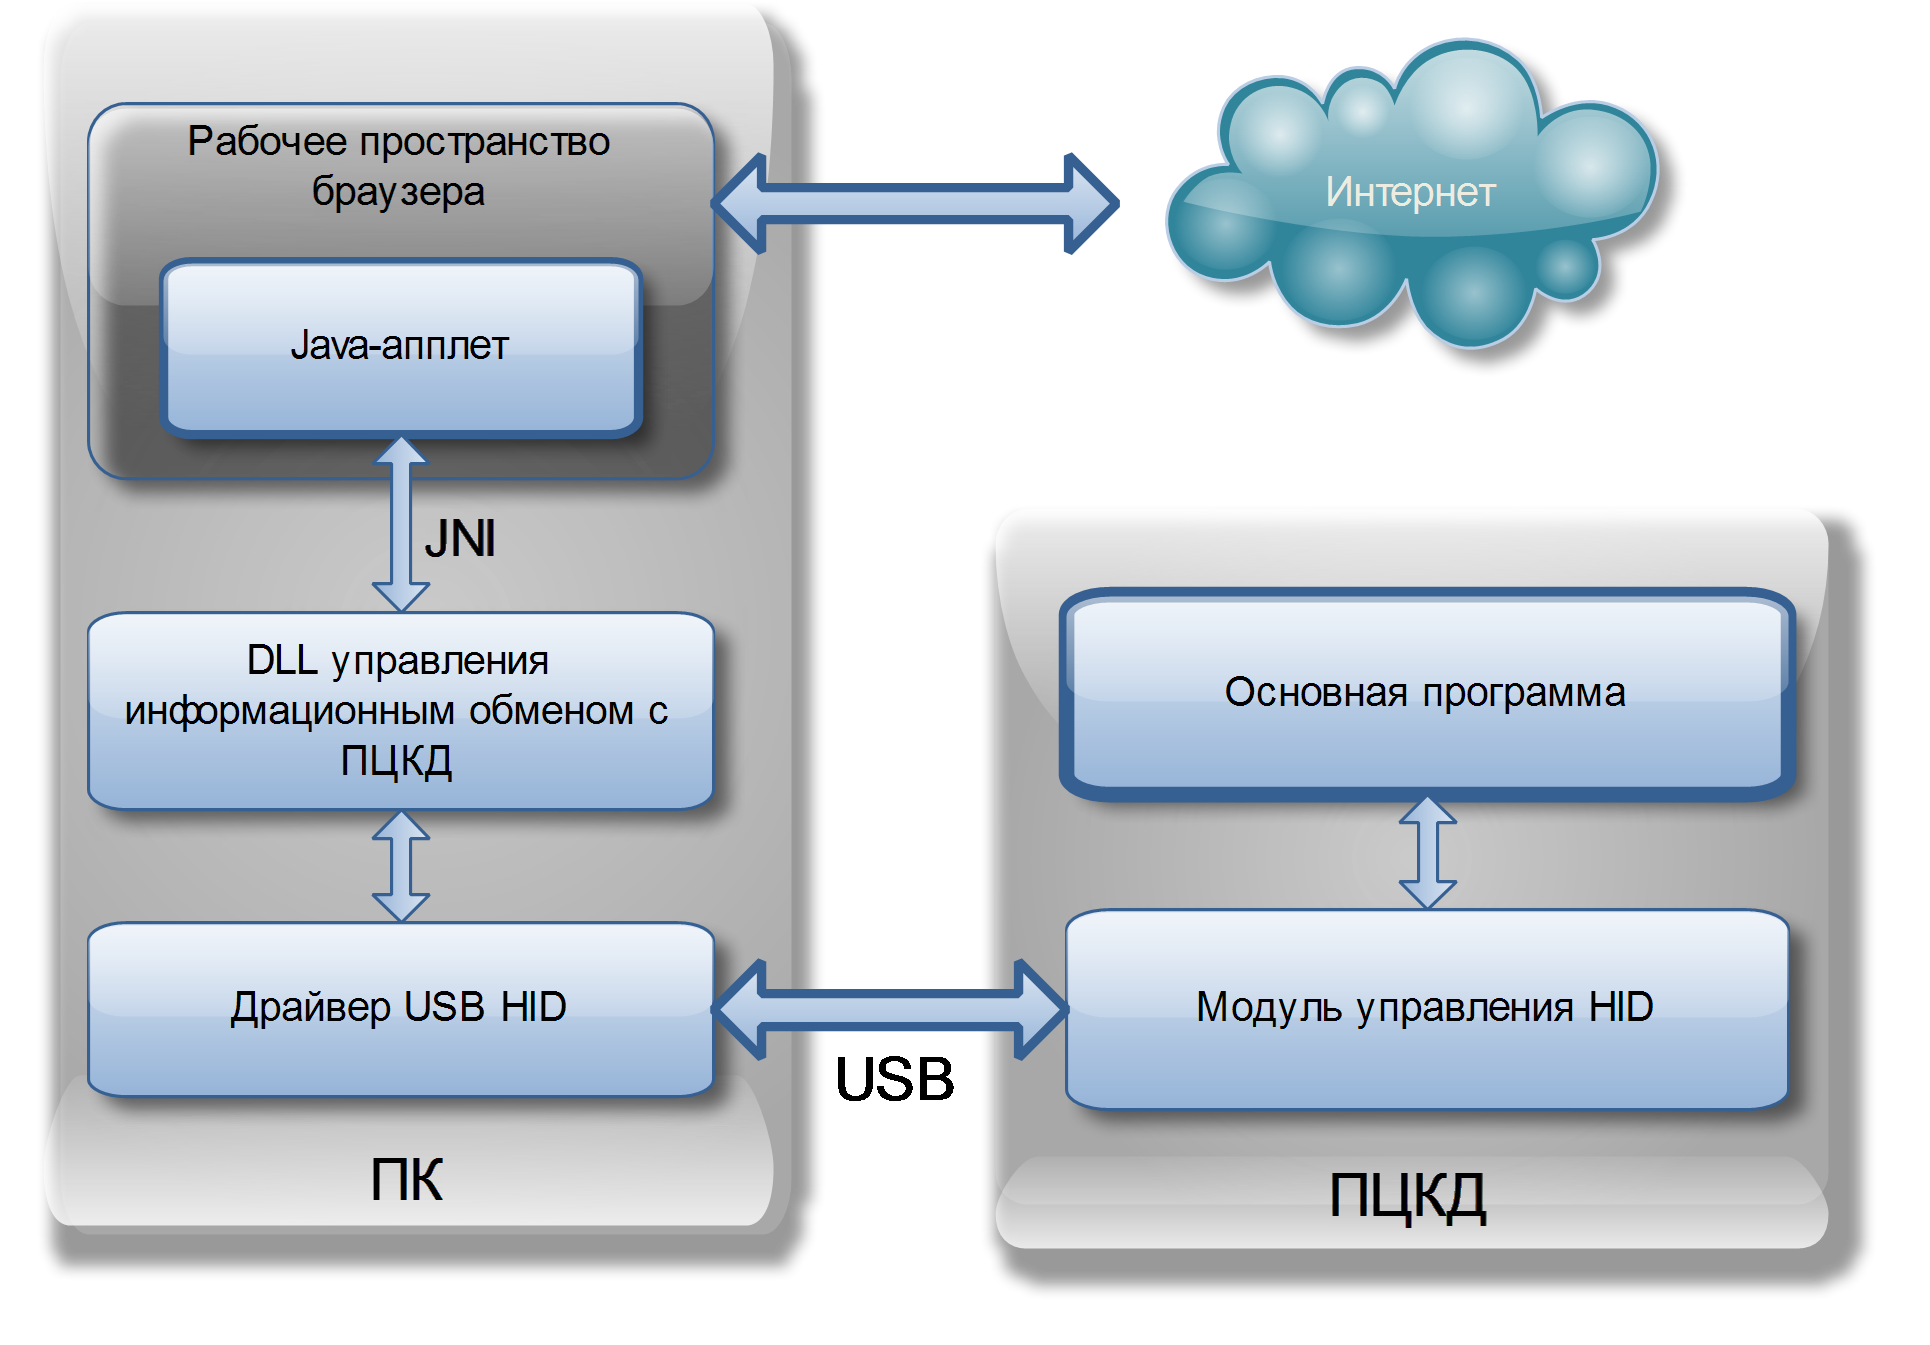
\includegraphics[width=1\linewidth]{3-3-3}}
\caption{Взаимодействие программных компонентов с использованием технологии
JavaApplet}
\label{ris:3.3.3}
\end{figure} 

Обязательным условием использования данного механизма является то, что
native-библиотека должна располагаться на диске машины клиента в специальной
директории. Следовательно, требуется инсталлировать библиотеку на
пользовательскую машину, после чего Java-апплет сможет подключить ее. Для этого
необходимо поместить Java-класс и библиотеку в jar-архив, который загрузится
вместе с html страницей. После чего, Java-апплет развернёт DLL-библиотеку во
временное хранилище машины пользователя и из него подгрузит DLL. Данную схему
иллюстрирует рисунок~\ref{ris:3.3.4}.

\begin{figure}[h!]
\center{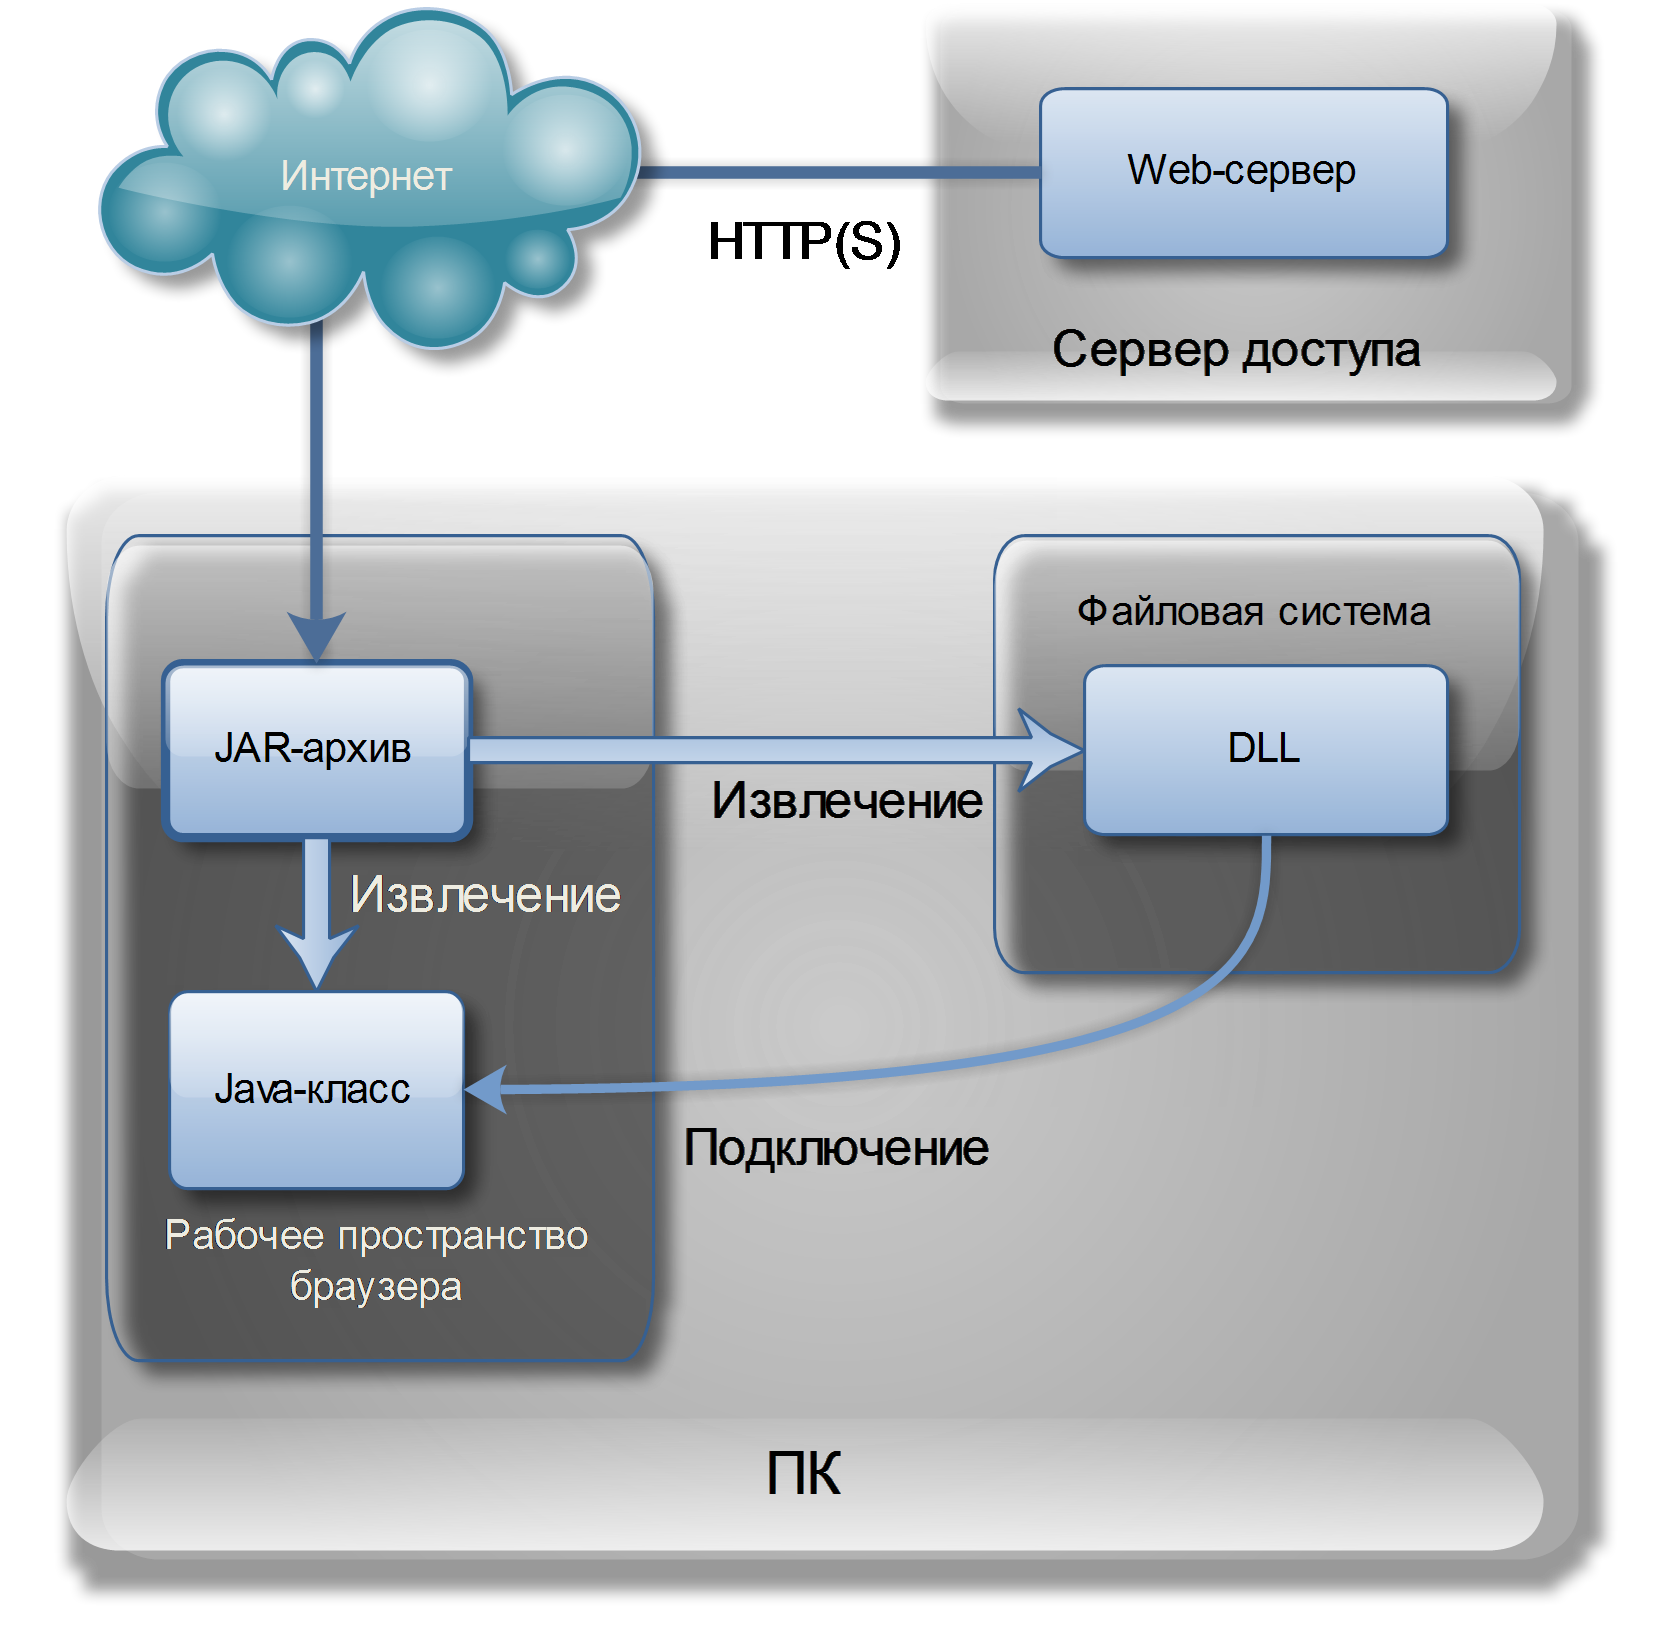
\includegraphics[width=1\linewidth]{3-3-4}}
\caption{Схема инсталляции библиотеки на клиентскую машину}
\label{ris:3.3.4}
\end{figure}  

В ходе развёртывания динамической библиотеки потребуется доступ к локальным
ресурсам пользователя (доступ к файловой системе). Java-апплету будет разрешён
доступ при условии его подписания электронно-цифровой подписью.~\cite{nikitin}

\subsection{Использование изложенных технических решений при построении системы доступа
к web-порталам с помощью ПЦКД}

В пункте~\ref{sect:concept} данной работы была рассмотрена схема
информационного обмена в процессе аутентификации пользователей в сети
корпоративных порталов.
Беря во внимание предложенные технические решения, упомянутая схема может быть
трансформирована в схему, приведенную на рисунке~\ref{ris:3.3.5}.
 
\begin{figure}[h!]
\center{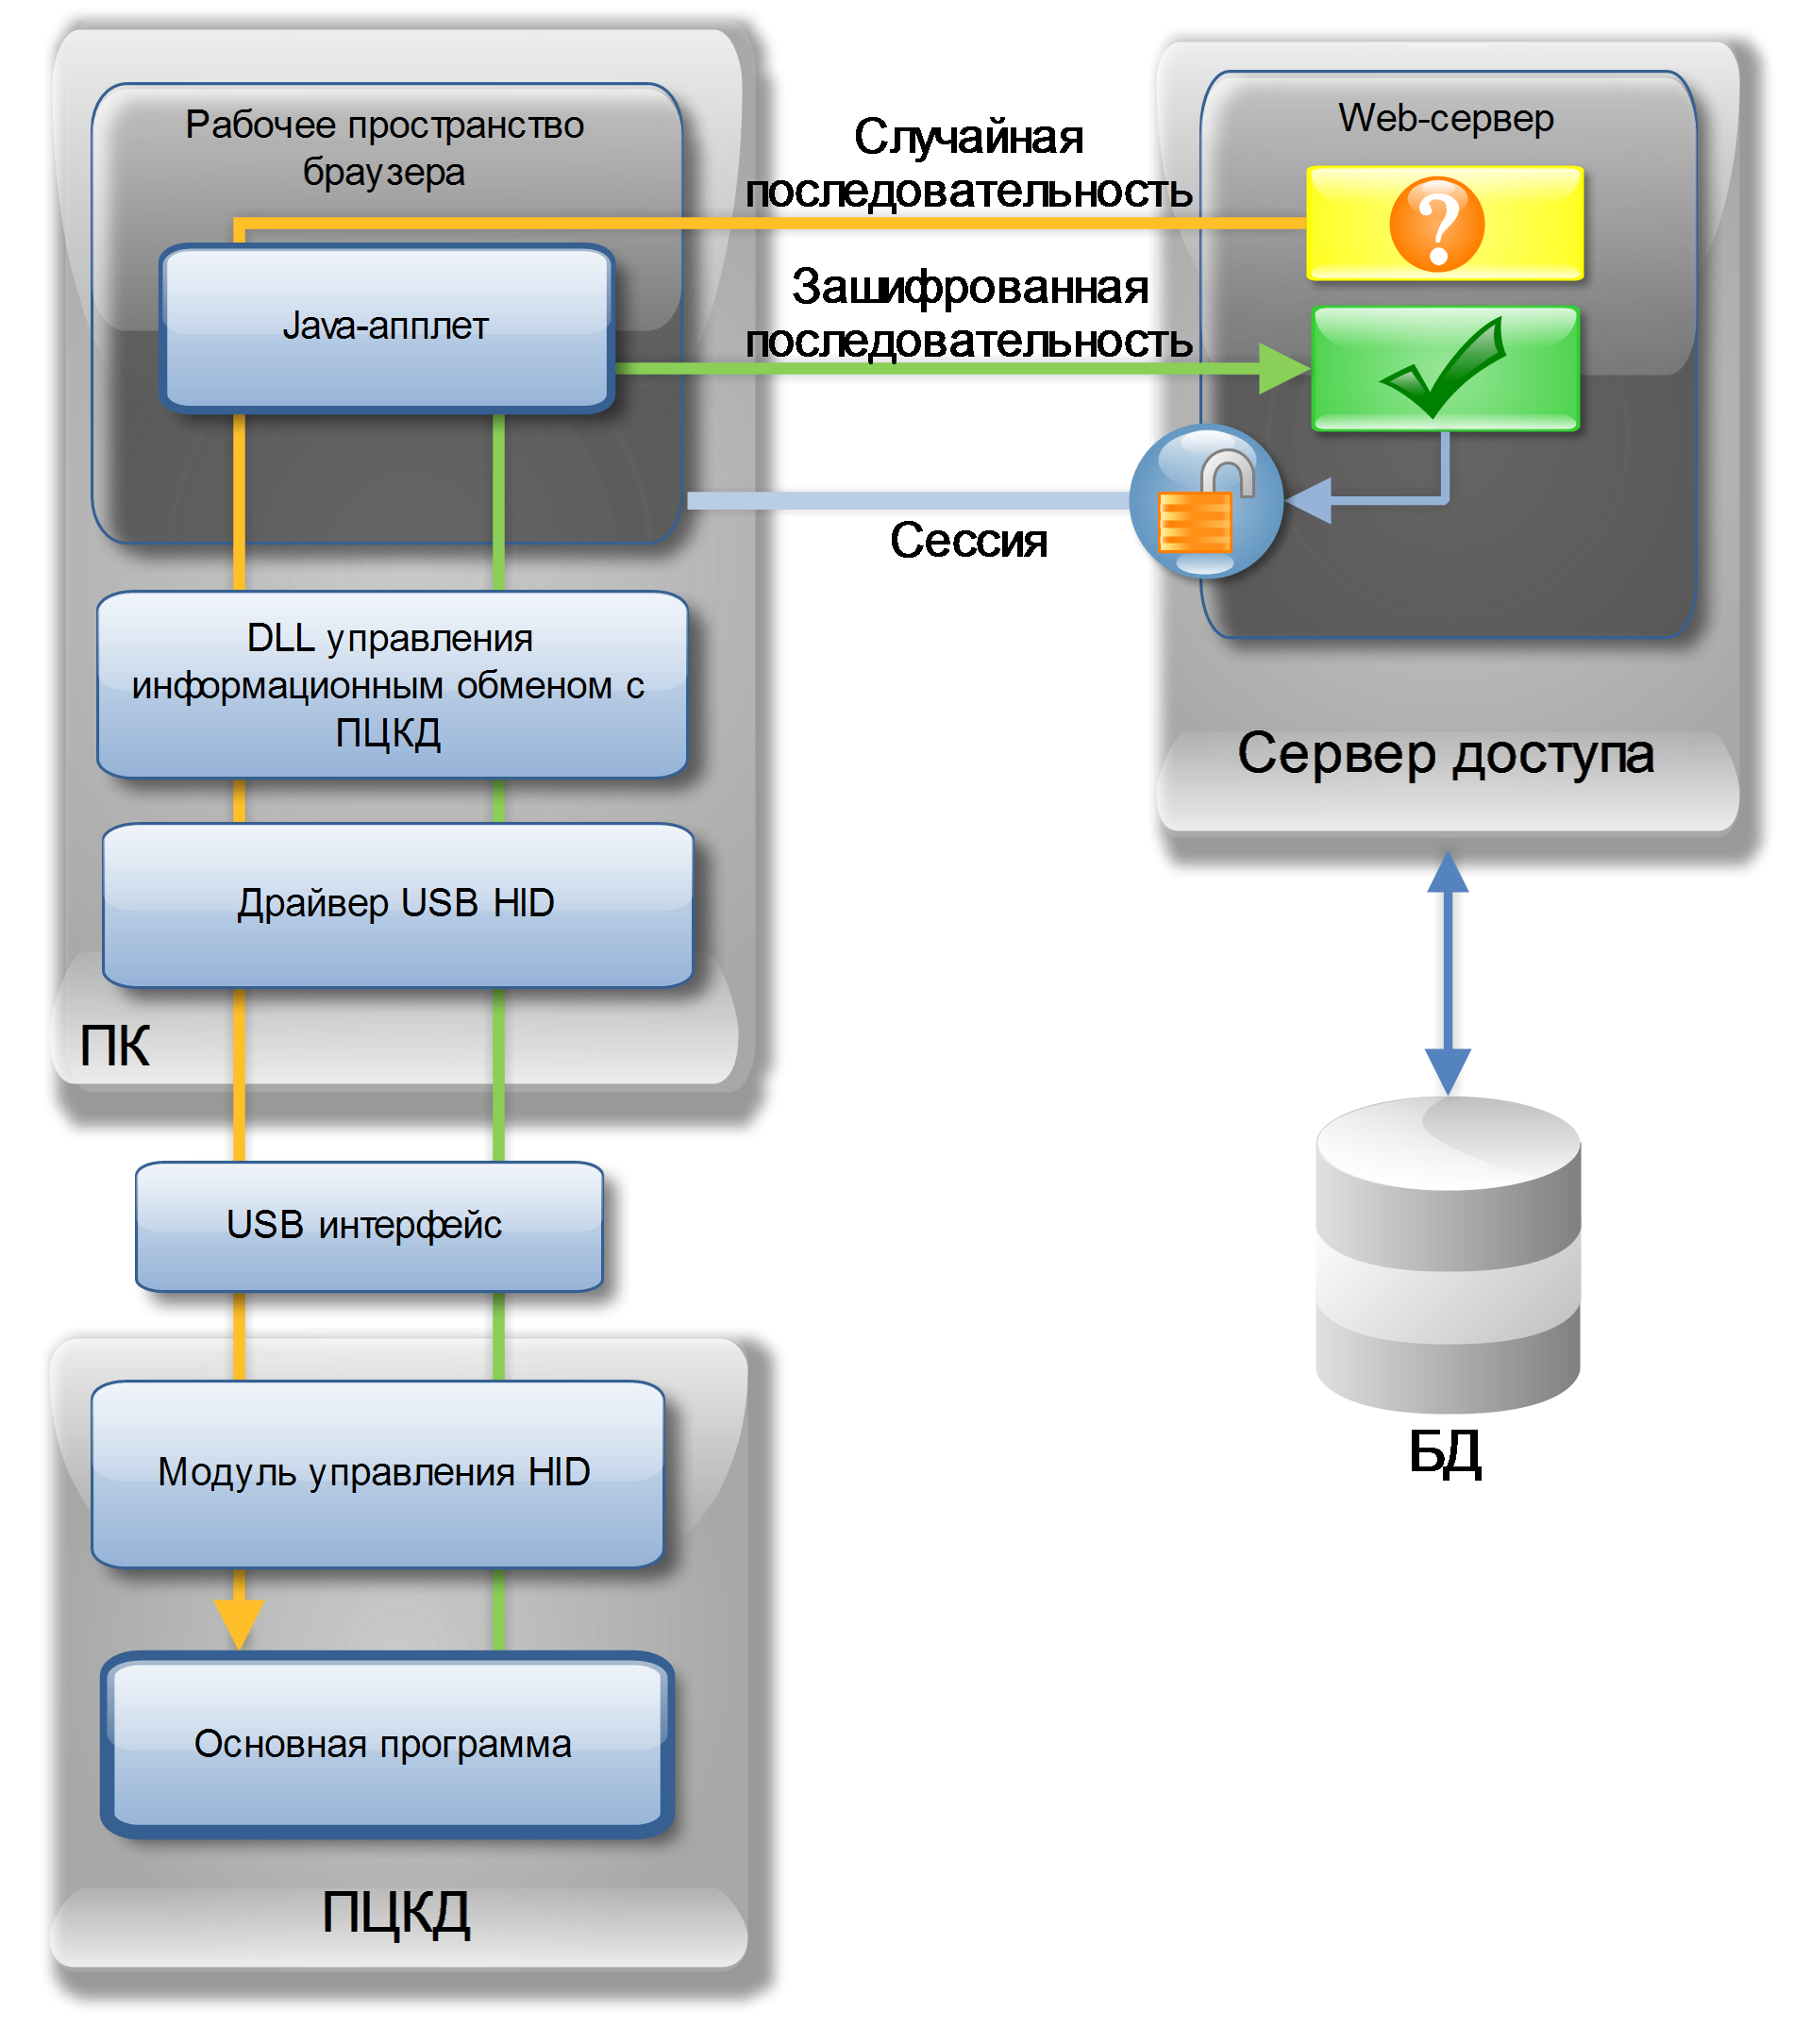
\includegraphics[width=1\linewidth]{3-3-5}}
\caption{Схема информационного обмена между пользователем и сервером доступа в
процессе аутентификации пользователей}
\label{ris:3.3.5}
\end{figure} 

При аутентификации пользователя в системе сервер отправляет случайную
последовательность битов, которые далее передаются в ПЦКД, реализуя предложенные
выше методы и технологии. После чего, ПЦКД шифрует полученную
последовательность, используя алгоритмы шифрования, а также секретный ключ, позволяющий однозначно
идентифицировать в системе пользователя – владельца ключа. Сгенерированный шифр
отправляется на сервер доступа, где проходит процедуру верификации. При
получении положительного ответа по окончании проверки, неизвестный признается
подлинным пользователем системы, в результате чего создаётся открытая сессия для
данного пользователя.~\cite{tex_asp}

\subsection{Описание протокола обмена данными высокого уровня с ПЦКД}

В соответствии с диаграммой активности, изображенной на
рисунках~\ref{ris:3.2.2}, ~\ref{ris:3.2.3}, а также, беря во
внимание схему на рисунке~\ref{ris:3.3.3} о взаимодействии программных и аппаратных компонентов
системы, можно утвержать, что существует необходимость в передаче разнородной
информации между ПК и ПЦКД.

Учитывая, что обмен данными по протоколу USB-HID осущаствляется через буфер,
который представляет собой массив байтов, возникает необходимость разработки
специального протокола обмена.

Исходя из функциональных требований к разрабатываемой подсистеме, можно выделить
действия, выполняемые ПЦКД:
\begin{enumerate}
  \item Получение от сервера, обработка и хранение секретного ключа;
  \item Вычисление сигнатуры (шифра) сообщения, полученного от сервера.
\end{enumerate}

В общем случае протокол входных данных можно представить в виде двух множеств:
$F$ -- множество функций и $P$ -- множество аргументов функций. Для каждой функции множество
аргументов $P$ может варьироваться. Множество $P$, в свою очередь,
трансформируется в тройку (формула~\ref{eq:set0}):

\begin{equation}
\label{eq:set}
<Q, S, D> ,
\end{equation}

где $Q$ -- множество параметров;

$S$ -- множество, значение ктоторого представлены в виде пары \textit{номер
аргумента -- размер в байтах};

$D$ -- множество аргументов;

\begin{equation}
\label{eq:set0}
\overbrace{f}^F \overbrace{\underbrace{q_1,q_2, \mbox{... } q_n}_Q
\underbrace{s_1,s_2, \mbox{... } s_m}_S \underbrace{(d_{1 1},d_{1 2}, \mbox{... }
d_{1 s_1});(d_{2 1},d_{2 2}, \mbox{... } d_{2 s_2}); \mbox{... } (d_{l 1},d_{l
2}, \mbox{... } d_{l s_m})}_D }^P
\end{equation}

Множества содержат незаконченый перечень значений.
Для первой функции (получение от сервера, обработка и хранение секретного
ключа) указанные подмножества (формула~\ref{eq:set}) могут принимать следующие
значения:

$Q = <q_1>$, где $q_1$ -- номер выбранного алгоритма шифрования;   

$D = <d_1, d_2>$, где $d_1$ -- шифр секретного ключа, $d_2$ -- идентификатор
пользователя в системе;

$S = <s_1, s_2>$, где $s_1$ и $s_2$ -- размер данных $d_1$ и $d_2$
соответственно.


Для второй функции (вычисление сигнатуры (шифра) сообщения, полученного от
сервера) подмножества аргументов~\ref{eq:set} могут принимать следующие
значения:

$D = <d_1>$, где $d_1$ -- сообщение, полученное клиентом;

$S = <s_1>$, где $s_1$ -- размер данных $d_1$.
\section{Интеграция решения по аутентификации пользователей в корпоративных
информационных системах с использованием ПЦКД}

Решение задачи интеграции клиентского решения по аутентификации и авторизации на
основе ПЦКД с корпоративными
информационными системами требует создания модуля адаптации, реализующего
непосредственное взаимодействие с интерфейсами информационных систем и имеющего
четкий протокол методов и параметров взаимодействия. Одним из возможных решений,
обеспечивающим универсальность и независимость клиентской части от архитектуры
самих корпоративных ИС является технология RPC (Remote Procedure Call или вызов
удаленных процедур).

\subsection{Технология RPC}
 
Идея вызова удаленных процедур состоит в расширении хорошо
известного и понятного механизма передачи управления и данных внутри программы,
выполняющейся на одной машине, на передачу управления и данных через сеть.
Средства удаленного вызова процедур предназначены для облегчения организации
распределенных вычислений. Наибольшая эффективность использования RPC
достигается в тех приложениях, в которых существует интерактивная связь между
удаленными компонентами с небольшим временем ответов и относительно малым
количеством передаваемых данных.

Характерными чертами вызова локальных процедур являются:
\begin{itemize}
  \item Асимметричность, то есть одна из взаимодействующих сторон является
инициатором;
\item Синхронность, то есть выполнение вызывающей процедуры при
останавливается с момента выдачи запроса и возобновляется только после возврата
из вызываемой процедуры.
\end{itemize}

Реализация удаленных вызовов существенно сложнее реализации вызовов локальных
процедур. Поскольку вызывающая и вызываемая процедуры выполняются на разных
машинах, то они имеют разные адресные пространства, и это создает проблемы при
передаче параметров и результатов, особенно если машины не идентичны. Так как
RPC не может рассчитывать на разделяемую память, то это означает, что параметры
RPC не должны содержать указателей на ячейки нестековой памяти и что значения
параметров должны копироваться с одного компьютера на другой. Следующим отличием
RPC от локального вызова является то, что он обязательно использует нижележащую
систему связи, однако это не должно быть явно видно ни в определении процедур,
ни в самих процедурах. Удаленность вносит дополнительные проблемы. Выполнение
вызывающей программы и вызываемой локальной процедуры в одной машине реализуется
в рамках единого процесса. Но в реализации RPC участвуют как минимум два
процесса -- по одному в каждой машине.~\cite{rpc}

К преимуществам технологии RPC
можно отнести следующее:
\begin{itemize}
  \item высокий уровень скрытия реализации процедур;
  \item широкие возможности для
встраивания различных подсистем;
\item гибкие возможности внесения изменений в
функционирование системы.
\end{itemize}

Взаимодействие программных компонентов при выполнении удаленного вызова
процедуры иллюстрируется рисунком~\ref{ris:3.4.1}. 

\begin{figure}[h!]
\center{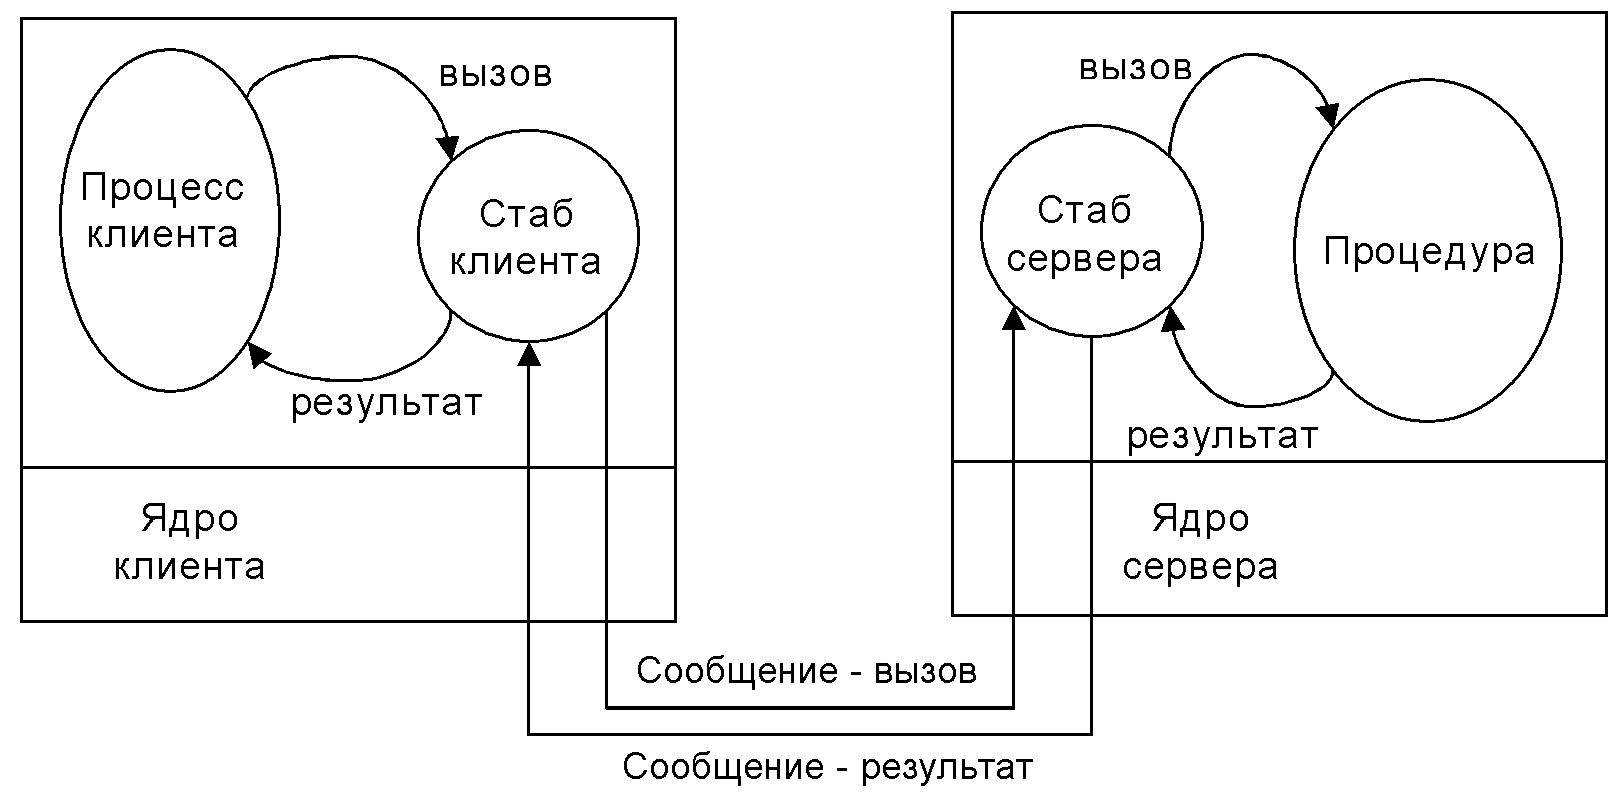
\includegraphics[width=1\linewidth]{3-4-1}}
\caption{Remote Procedure Call}
\label{ris:3.4.1}
\end{figure}

После того, как клиентский стаб (stub -
заглушка) был вызван программой-клиентом, его первой задачей является заполнение
буфера отправляемым сообщением. В некоторых системах клиентский стаб имеет
единственный буфер фиксированной длины, заполняемый каждый раз с самого начала
при поступлении каждого нового запроса. В других системах буфер сообщения
представляет собой пул буферов для отдельных полей сообщения, причем некоторые
из этих буферов уже заполнены. Этот метод особенно подходит для тех случаев,
когда пакет имеет формат, состоящий из большого числа полей, но значения многих
из этих полей не меняются от вызова к вызову.
Затем параметры должны быть преобразованы в соответствующий формат и вставлены в
буфер сообщения. К этому моменту сообщение готово к передаче, поэтому
выполняется прерывание по вызову ядра.

Когда ядро получает управление, оно переключает контексты, сохраняет регистры
процессора и карту памяти (дескрипторы страниц), устанавливает новую карту
памяти, которая будет использоваться для работы в режиме ядра. Поскольку
контексты ядра и пользователя различаются, ядро должно точно скопировать
сообщение в свое собственное адресное пространство так, чтобы иметь к нему
доступ, запомнить адрес назначения (а, возможно, и другие поля заголовка), а
также оно должно передать его сетевому интерфейсу. На этом завершается работа на
клиентской стороне. Включается таймер передачи, и ядро может либо выполнять
циклический опрос наличия ответа, либо передать управление планировщику, который
выберет какой-либо другой процесс на выполнение. В первом случае ускоряется
выполнение запроса, но отсутствует мультипрограммирование.

На стороне сервера поступающие биты помещаются принимающей аппаратурой либо во
встроенный буфер, либо в оперативную память. Когда вся информация будет
получена, генерируется прерывание. Обработчик прерывания проверяет правильность
данных пакета и определяет, какому стабу следует их передать. Если ни один из
стабов не ожидает этот пакет, обработчик должен либо поместить его в буфер, либо
вообще отказаться от него. Если имеется ожидающий стаб, то сообщение копируется
ему. Наконец, выполняется переключение контекстов, в результате чего
восстанавливаются регистры и карта памяти, принимая те значения, которые они
имели в момент, когда стаб сделал вызов receive.

Теперь начинает работу серверный стаб. Он распаковывает параметры и помещает их
соответствующим образом в стек. Когда все готово, выполняется вызов сервера.
После выполнения процедуры сервер передает результаты клиенту. Для этого
выполняются все описанные выше этапы, только в обратном порядке.

\subsection{Общая схема интеграции модулей ПЦКД в корпоративные ИС}

Рассмотрев специфику взаимодействия программных компонентов системы
аутентификации с применением ПЦУД, была предложена схема (рисунок~\ref{ris:3.4.2})
интеграции клиентских программных компонентов в сервер доступа, используя технологию RPC.

\begin{figure}[h!]
\center{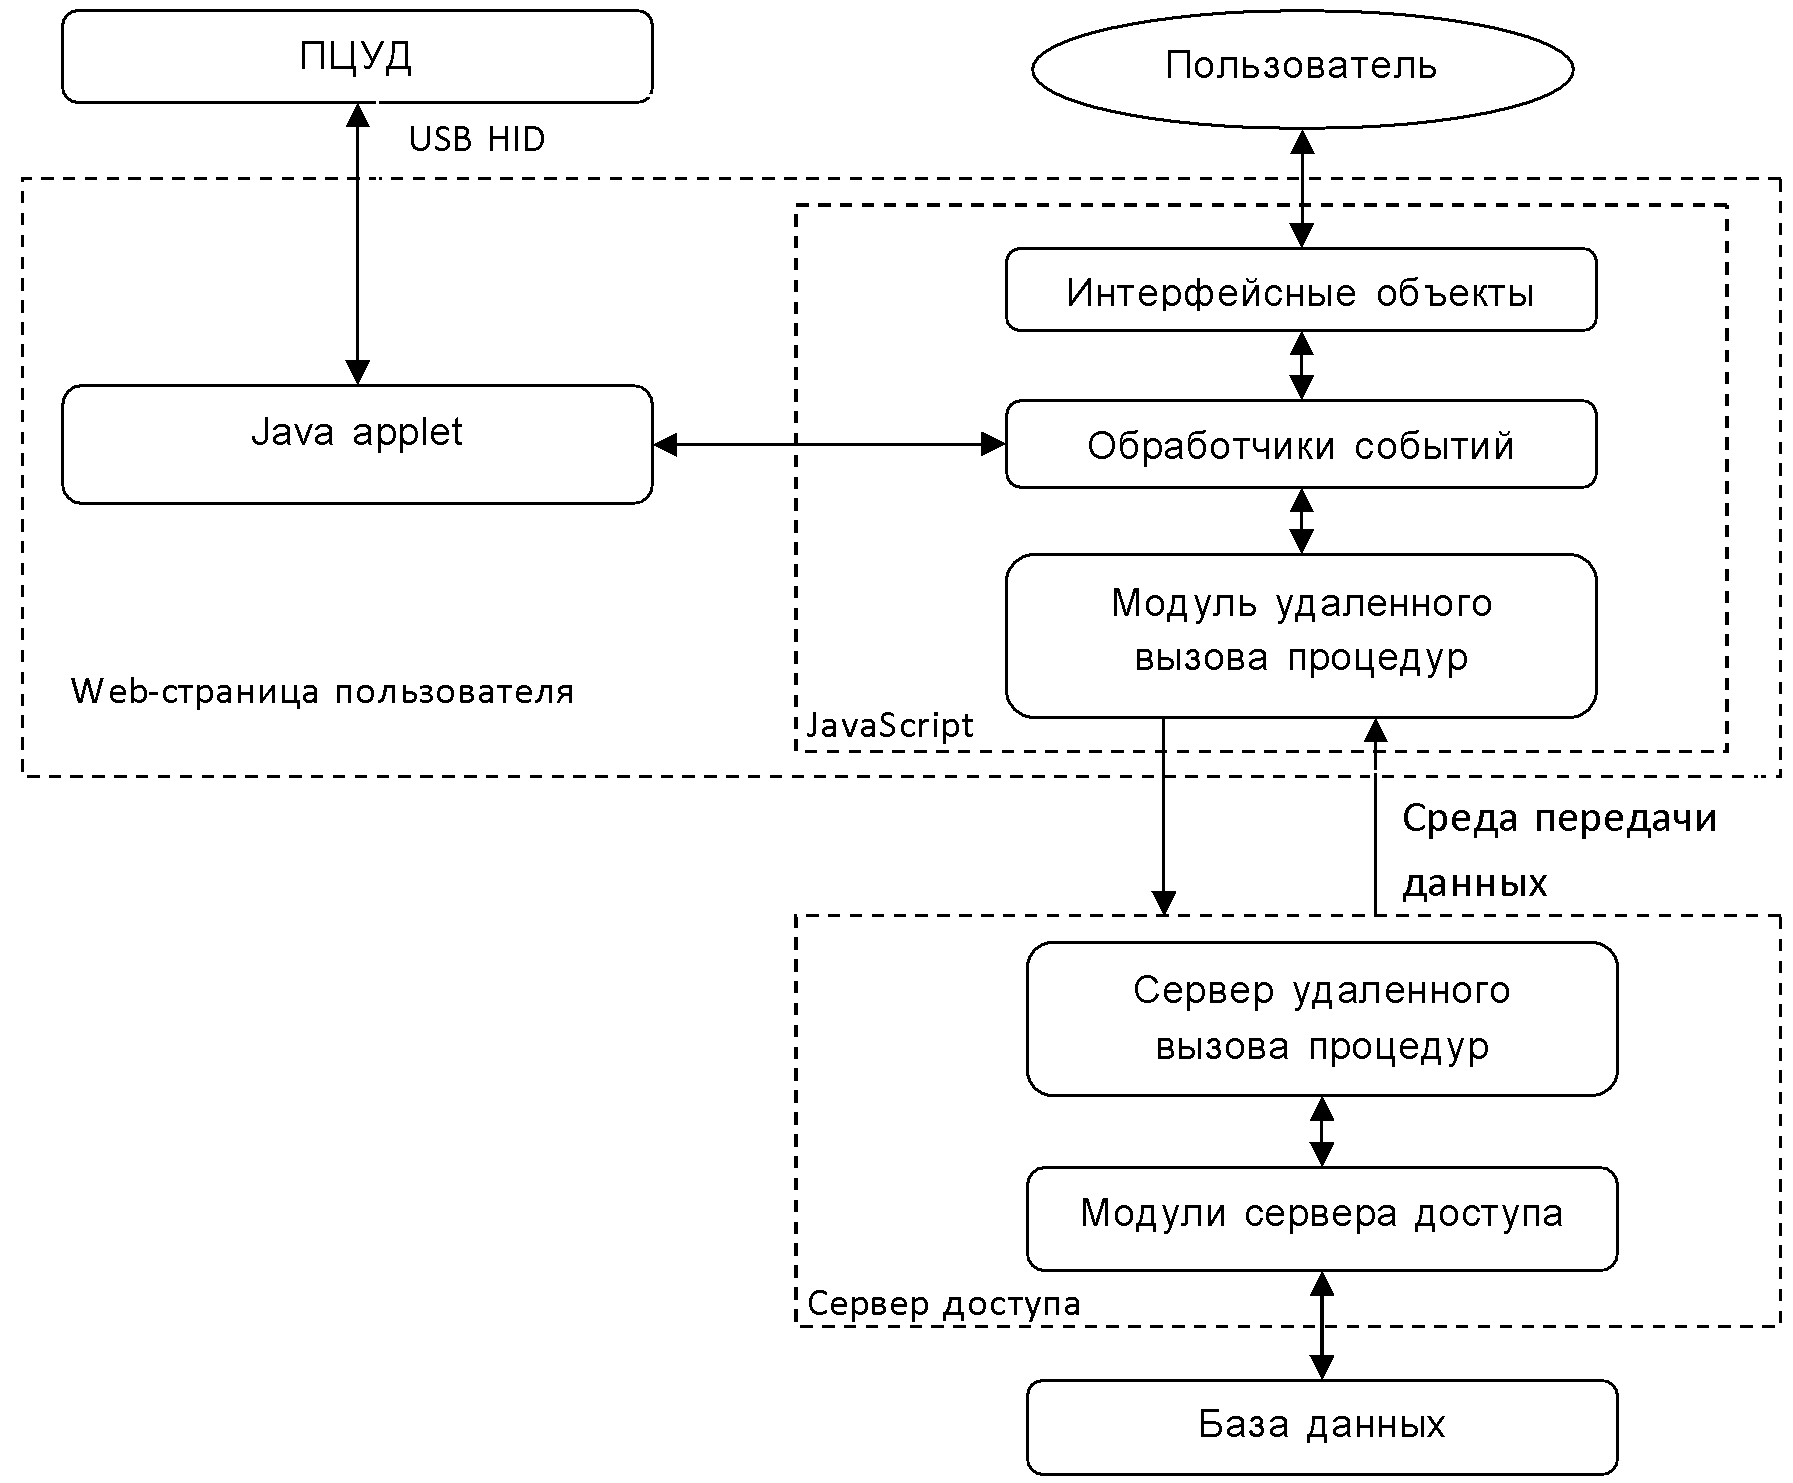
\includegraphics[width=1\linewidth]{3-4-2}}
\caption{Схема интеграции клиентского решения на основе ПЦКД с серверами
контроля доступа, используя технологию RPC}
\label{ris:3.4.2}
\end{figure} 

В соответствии с данной схемой можно выделить 4 сущности:
\begin{itemize}
  \item пользователь;
  \item web-страница пользователя;
  \item пользовательский ключ (ПЦКД);
  \item сервер доступа.
\end{itemize}

В Web-страницу встраивается Java-апплет и JavaScript. Java-апплет образует
магистраль передачи данных фиксированного формата в ПЦУД, подключенное к ПК по
интерфейсу USB-HID. JavaScript имеет описание и заголовки удаленных процедур,
физически размещенных на сервере доступа. По имеющимся заголовкам JS может
осуществлять удаленный вызов процедур, а так же передавать параметры и
обрабатывать результат. Для инициирования выполнения конкретной процедуры со
стороны пользователя, существуют интерфейсные объекты (кнопки, поля для ввода и
т.п.) и связанные с ними обработчики событий.
При появлении новой функции на сервере, достаточно определить интерфейсный
объект и привязать к нему обработчик события, после чего пользователь сможет
вызвать необходимую процедуру.
Наличие или отсутствие интерфейсных объектов может регулировать уровень доступа
на основе списка прав. Необходимый набор интерфейсных объектов описывает тот или
иной уровень прав доступа в соответствии с разрешениями для данного
пользователя.~\cite{art_rpc}

\subsection{Реализация механизма RPC}

При реализации механизма удаленного вызова процедур применительно к системе
аутентификации пользователей в сети корпоративных порталов с использованием
ПЦУД, было предложено задействовать одно из стандартных средств -- SimpleAjax
(SAJAX).

Sajax представляет собой инструмент с открытым исходным кодом, чтобы сделать
программирование веб-сайтов с помощью платформы Ajax как можно проще. Sajax
делает это при помощи вызова PHP, Perl, ColdFusion, IO, LUA, Ruby или Python
функций с помощью JavaScript без обновления web-страницы.~\cite{sajax} По факту
SimpleAjax выполняет асинхронные HTTP запросы (GET или POST) к удаленному
серверу передавая в качестве параметров заголовки процедур, предварительно
упакованных в формат XML. Общий формат вызываемой процедуры выглядит следующим
образом:

\begin{center}
  \textit{Call(procedure, [arguments], [callback]),} где 
 \end{center} 
 
 \textbf{procedure} --- обязательный параметр: строка, имя
 вызываемой процедуры;

\textbf{arguments} --- необязательный параметр: объект, аргументы вызываемой
процедуры;

\textbf{callback} --- необязательный параметр: функция принимающая объект,
реализует обработку ответа.

Содержимое данной процедуры преобразуется в формат XML, и далее передается на
сервер, где происходит обработка XML-объекта и выполнение удаленной процедуры.
При наличии возвращаемых параметров, они так же преобразуются в XML-объект,
который возвращается клиенту, где происходит его обработка.

Для выполнения заявленных функциональных требований, серверная часть подсистемы
должна реализовывать ряд функций~\ref{alg:2}, которые можно условно объединить в
следующие категории:
\begin{enumerate}
  \item Функции для управления пользователями и ключами (\textit{MakeUser,
  \\ ChangeKey});
  \item Функции для аутентификации пользователя (\textit{GetSoul, SetSession});
  \item Функции для выполнения документооборота \textit{(LoadFile, SignFile}).
\end{enumerate}

\begin{algorithm}[ht]
\floatname{algorithm}{Алгоритм}                
\caption{Описание функций клиентской части, физически размещенных на сервере
(RPC)}
\label{alg:2}     
\small                    
\begin{algorithmic}

\Procedure {MakeUser}{$username$} \Comment{Создание пользователя}

\Return{$massage$} \Comment{Шифрованное сообщение, содержащее ключ для ПЦКД}
\EndProcedure

\Procedure {ChangeKey}{$userid$} \Comment{Изменение ключа для
ПЦКД пользователя}

\Return{$massage$} \Comment{Шифрованное сообщение, содержащее ключ для ПЦКД}
\EndProcedure

\Procedure {GetSoul}{$void$} \Comment{Получение случайного
сообщения на сервере}

\Return{$Soul$} \Comment{Случайная последовательность}
\EndProcedure
  
\Procedure {SetSession}{$userid, signature$}  \Comment{Установка
сессии}

\Return{$CookieHash$} \Comment{CookieHash -- идентификатор сессии}
\EndProcedure

\Procedure {LoadFile}{$file, userid$}  \Comment{Загрузка файла на
сервер}
\EndProcedure

\Procedure {SignFile}{$filehash, signature$}  \Comment{Подписание
файла}
\EndProcedure

\end{algorithmic}
\end{algorithm}

Реализация механизма RPC, а также приведенных функций указана в
приложении~\ref{pril:C}.
\section{Модель данных}

Для интеграции подсистемы аутентификации с применением ПЦКД в корпоративную
информационую систему необходима база данных для хранения пользовательской
информации и обеспечения функционирования серверных модулей. На
рисунке~\ref{ris:3.5} представлейна минимальная схема базы данных, необходимая
для успешной интеграции данной подсистемы. Предложенная модель построена по
принципу <<необходимости, но недостаточности>> и может быть расширена другими
сущностями, необходимыми для работы конкретной корпоративной информационной
системы.

\begin{figure}[h!]
\center{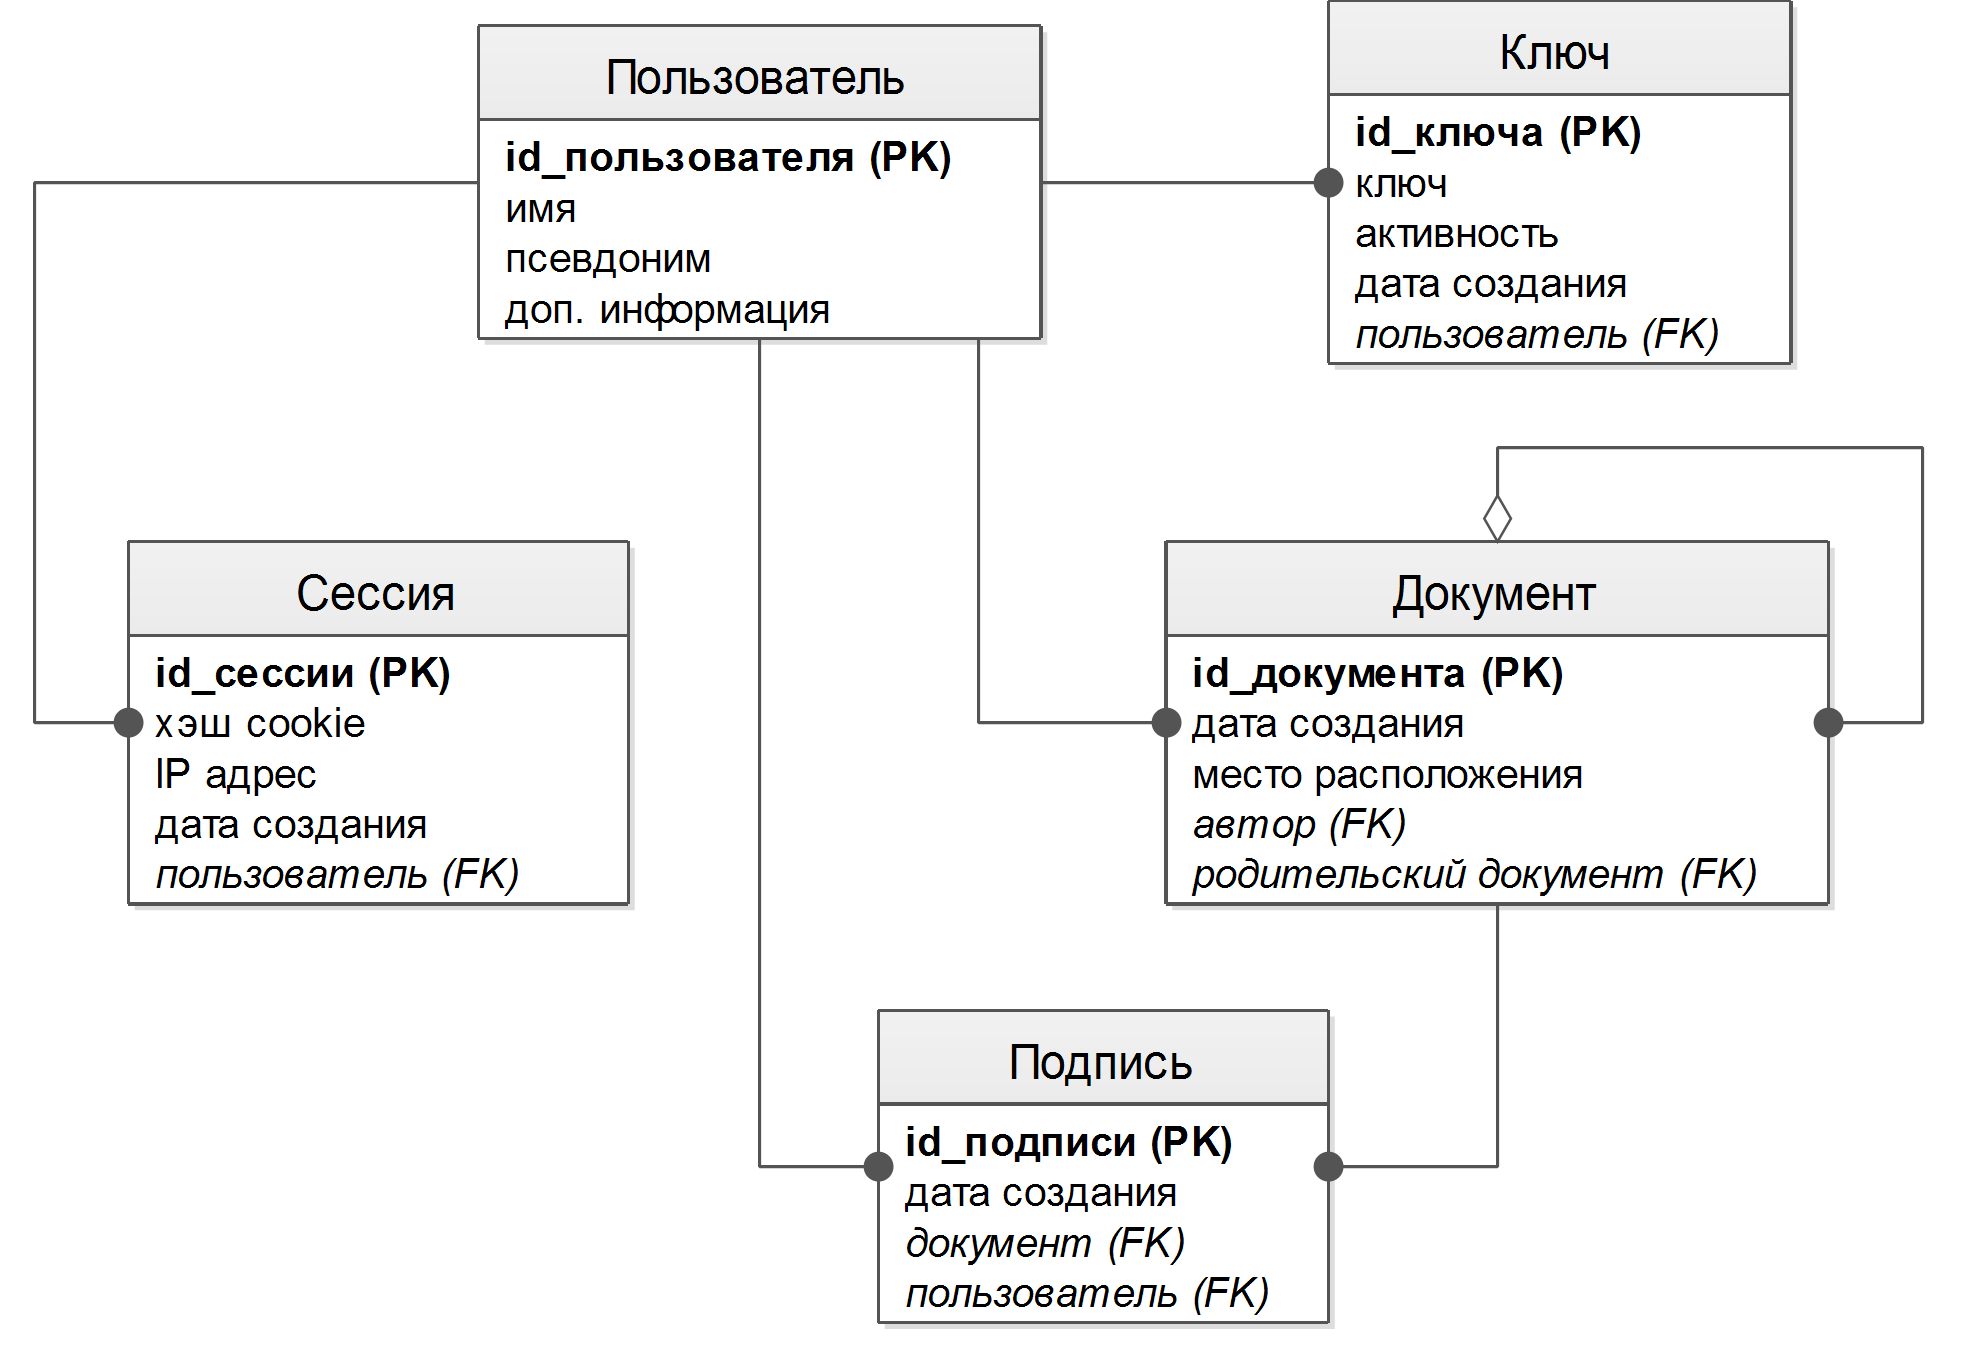
\includegraphics[width=1\linewidth]{3-5}}
\caption{Концептуальная модель данных}
\label{ris:3.5}
\end{figure}

Центральной сущностью концептуальной модели данных является
сущность <<Пользователь>>, так как от нее отталкиваются другие объекты.
Данная сущность описывает пользователя системы и имеет атрибуты:
\begin{itemize}
  \item идентификатор пользователя -- первичный ключ;
  \item имя;
  \item дополнительная информация, характеризующая пользователя (телефонный
  номер, адрес электронной почты).
\end{itemize}

Сущность <<Пользователь>>, теоретически, может быть позаимствована из уже
существующей базы данных, установив соответствие между идентификатором
пользователя и связанными с ним объектами.

Сущность <<Ключ>> описывает информацию, касаемую секретных ключей и имеет
следующие атрибуты:

\begin{itemize}
  \item идентификатор ключа -- первичный ключ;
  \item ключ;
  \item активность -- указывает на возможность использования данного ключа;
  \item дата создания.
\end{itemize}

Каждый пользователь может иметь неограниченное количество ключей, но в
конкретный момент активным может быть только один. Поэтому должен быть
предусмотрен триггер, ведущий слежение за активностью ключей, а так же их
деактивацию при истечении срока службы.

Сущность <<Сессия>> описывает информацию, необходимую для поддержания
пользовательского сеанса. Так же ее можно использовать для ведения учета
посещаемости пользователей (аккаунтинг).

Сущность <<Документ>> описывает файлы, размещаемые пользователем для
осуществления электронного документаоборота. Данная сущность имеет следующие
атрибуты:

\begin{itemize}
  \item идентификатор документа -- первичный ключ;
  \item место расположения -- указывает на адрес размещения файла;
  \item дата создания.
\end{itemize}

\begin{algorithm}[h!]
\floatname{algorithm}{Алгоритм}                 % enter the algorithm
\caption{Функционирование ПЦКД}          % give the algorithm a caption
\label{alg:1}     
\small                      % and a label for \ref{} commands later in the
% document
\begin{algorithmic}[1]      
\State $n \gets 64$ \Comment{размер буфера обмена в байтах}
\State $page \gets 1024$ \Comment{page -- адресс памяти}
\Loop
  \State $iBuf \gets $ \Call{Чтение входного буфера}{void}
  \If{$iBuf$ НЕ пустой}
    \If{$iBuf[0] = 1$} \Comment{Вычисление сигнатуры}
      \State $pBuf \gets $ \Call{Чтение из внутренней flash-памяти}{page}
      \State $alg \gets pBuf, id \gets pBuf, secret \gets bBuf, message \gets
      pbuf$ \Comment{Парсинг pBuf: alg -- алгоритм, id -- идентификатор
      пользователя а системе, secret -- закытый ключ, message -- входное сообщение}
      \State $tBuf \gets$ \Call {Вычисление сигнатуры}{message, secret, alg}
      \Comment{В соответствии с заданным алгоритмом шифрования}
      \State $oBuf \gets tBuf + id$ \Comment{Конкатенация массивов}
    \EndIf    
    
    \If{$iBuf[0] = 2$} \Comment{Запись параметров в память}
      
      \State $pBuf[0..n-1] \gets iBuf[1..n]$
      \State $pBuf \gets $ \Call{Расшифровка}{pBuf, key} \Comment{key -- ключ
      расшифровки } \State \Call{Запись во внутреннюю flash-память}{pBuf,
      page}
      \State $pBuf[0..n] \gets 0$ \Comment{Тестирование записи}
      \State $pBuf \gets $ \Call{Чтение из внутренней flash-памяти}{page}
      \State $oBuf \gets pBuf$
    \EndIf
    
    \State Запись в выходной буфер ($oBuf$)
  \EndIf
\EndLoop

\end{algorithmic}
\end{algorithm}

Данная сущность является рекурсивной. Это исходит из того факта, что каждый
документ может иметь потомков, то есть документов, полученных на основе данного,
путем изменения и редактирования.

Сущность <<Подпись>> описывает информацию, предназначенную для подтверждения
подлинности документов. Данные для данной сущности поступают от клиентских
компонентов системы и извлекаются в процессе верификации.

\section{Алгоритмы}

В результате проектирования, на основании технического решения, было разработано
множество алгоритмов для различных узлов подсистемы. Наиболее интересным и
показательным является алгоритм~\ref{alg:1}, демонстрирующий последовательность
действий главного блока программы портативного цифрового ключа доступа.
\chapter{Реализация системы}

На завершающей стадии выполнения работы был реализован опытный образец
портативного цифрового ключа доступа. Фотографии данного опытного
образца представлены на рисунке~\ref{ris:4.0.1}.

\begin{figure}[ht]
\begin{center}

\begin{minipage} [h]{0.8\linewidth}
\center{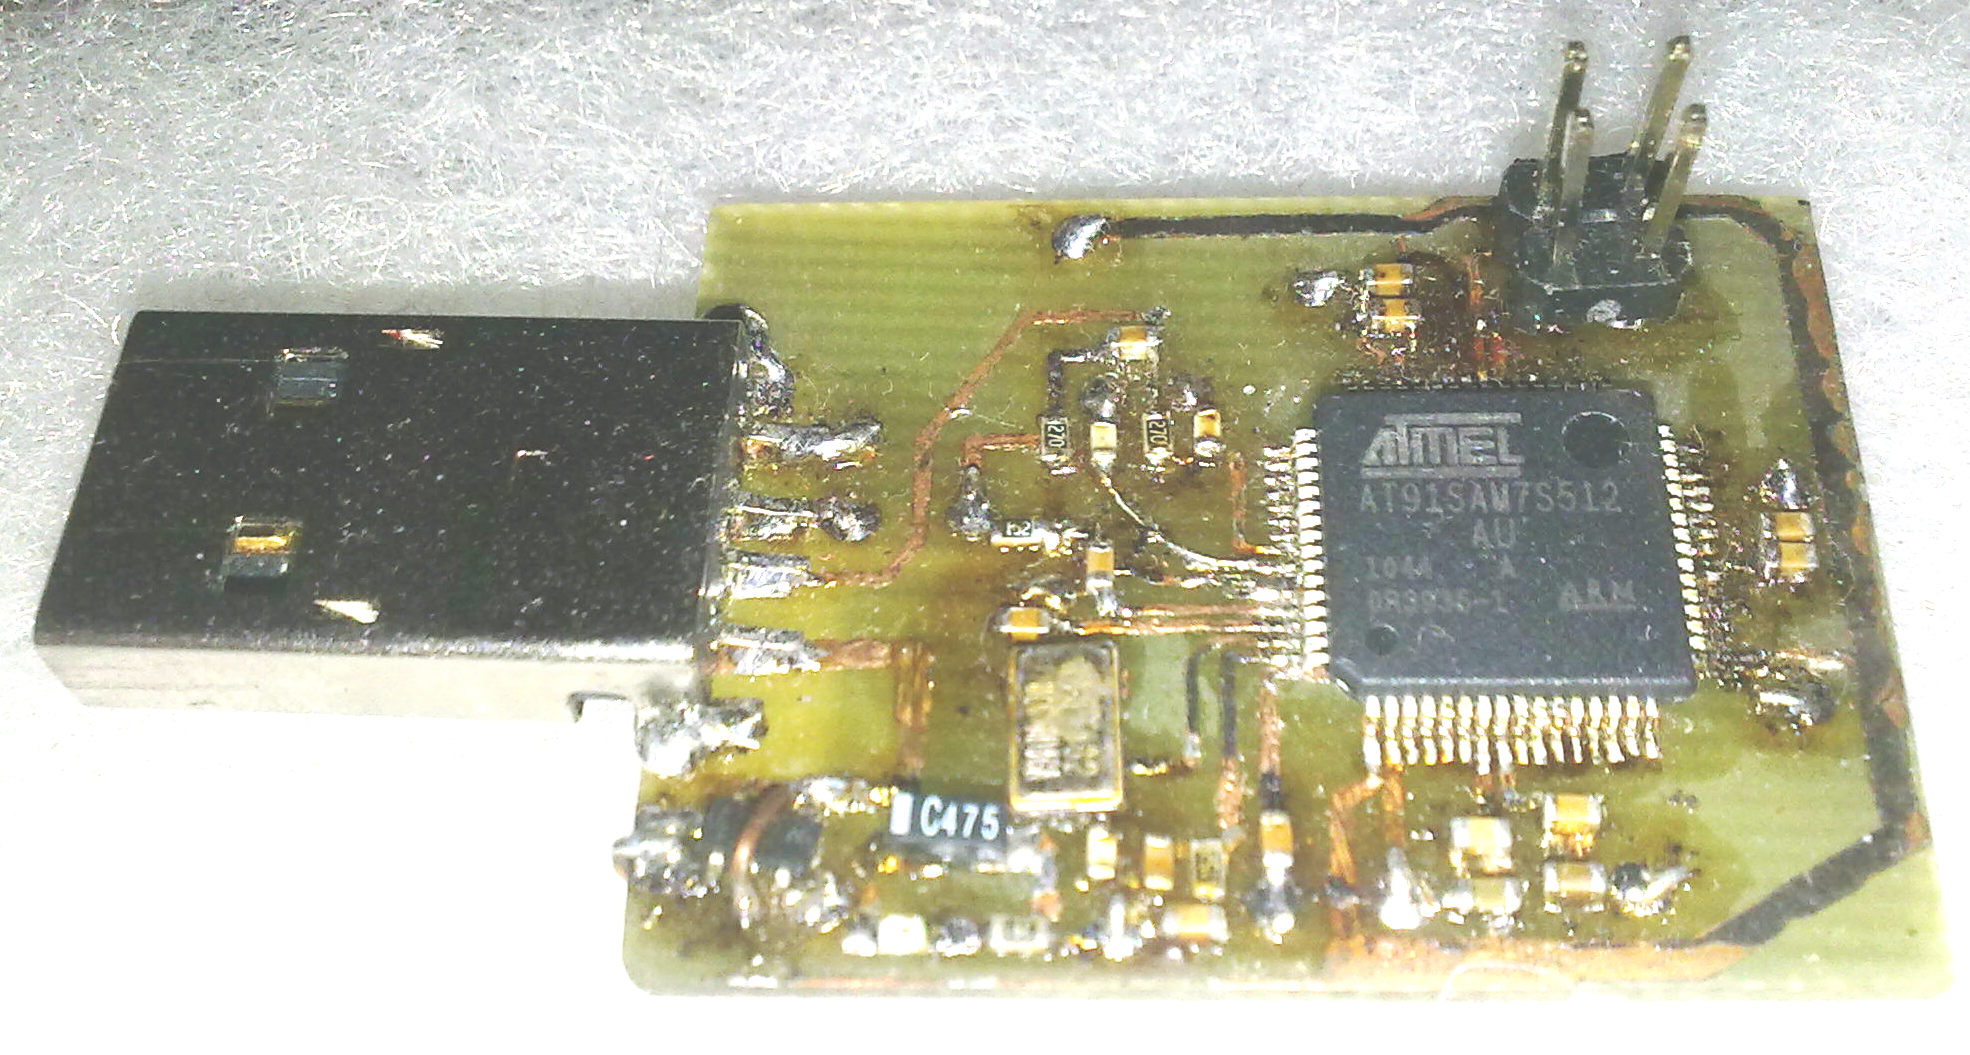
\includegraphics[width=1\linewidth]{4-0-1} \small{Вид под углом} \\ }
\end{minipage}
\hfill
\begin{minipage} [h]{0.8\linewidth}
\center{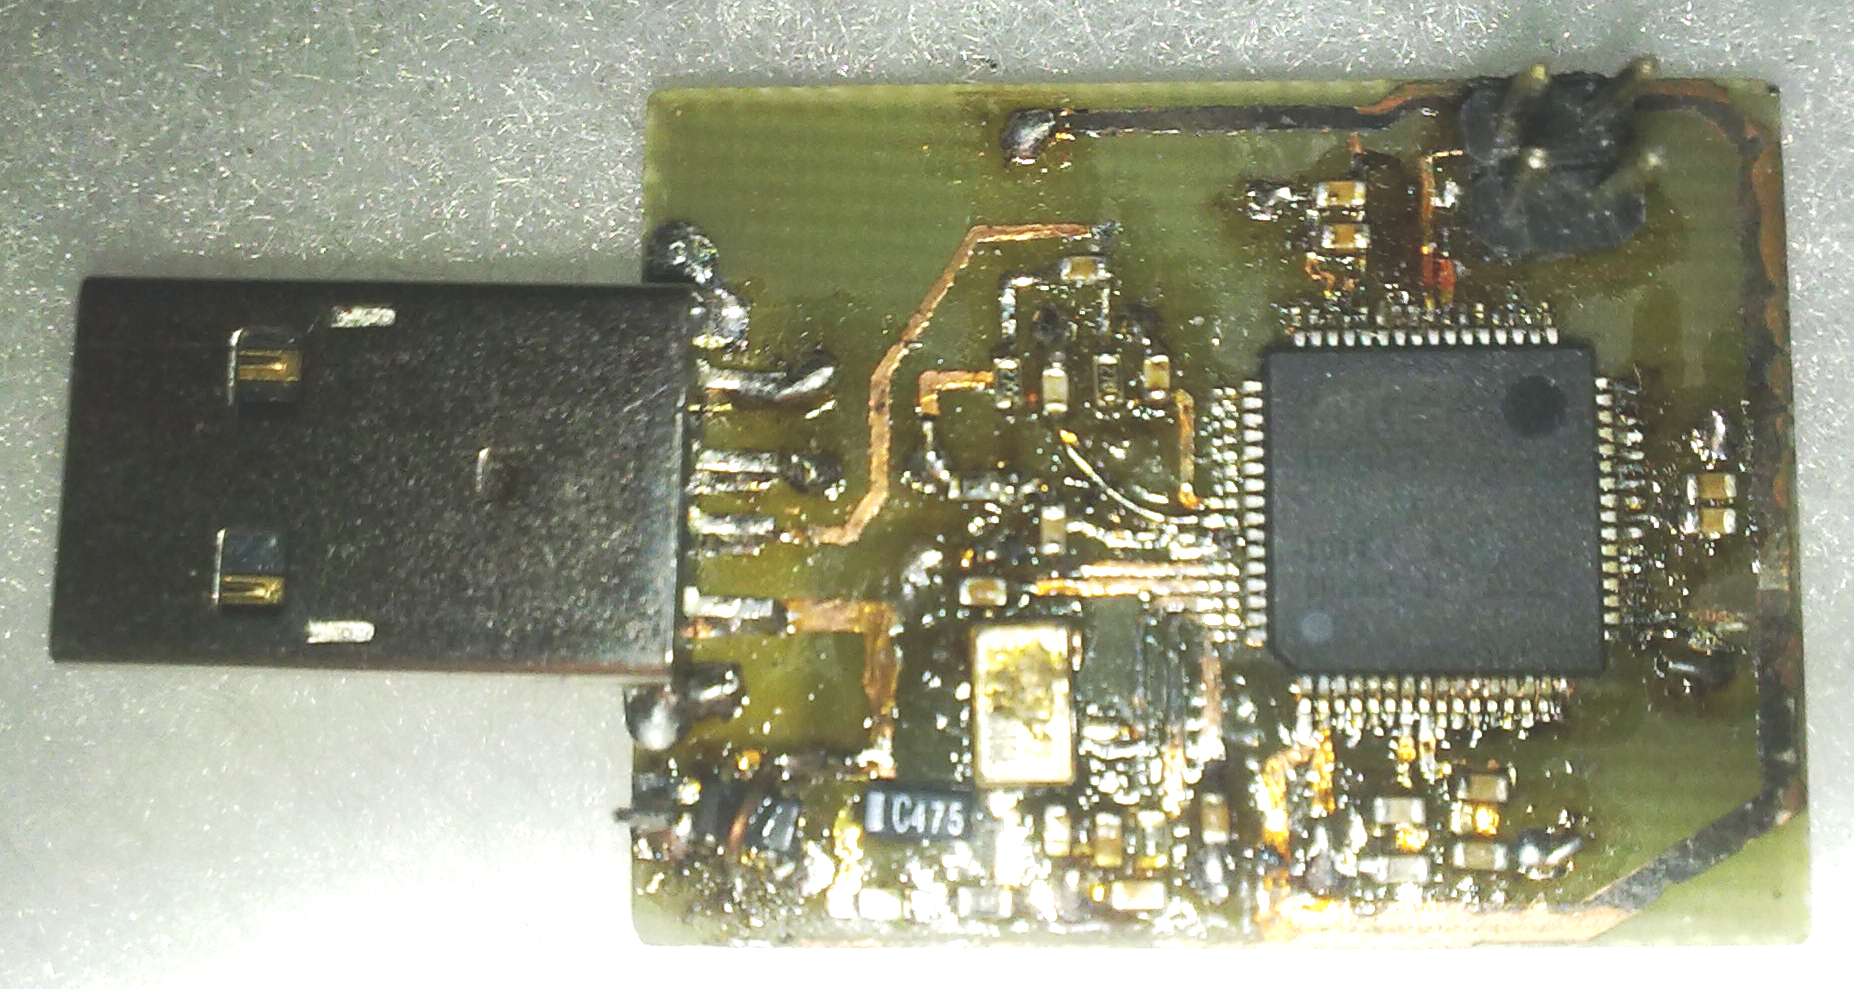
\includegraphics[width=1\linewidth]{4-0-2} \\
\small{Вид сверху}}

\end{minipage}
\end{center}
\caption{Фотография прототипа ПЦКД}
\label{ris:4.0.1}
\end{figure}

Данное устройство выполнено в форм-факторе <<USB-флешки>>,
без применения промышленных технологий (методом ручной сборки).

Так же была создана и зарегистрирована программа, на основе проектного решения
являющаяся подсистемой аутентификации пользователей в сети КИП на основе
портативного цифрового ключа доступа.~\cite{svidetelstvo_auth}. Листинг кода
данной программы представлен в приложении~\ref{pril:B}. На
рисунке~\ref{ris:4.0.3}, рисунке~\ref{ris:4.0.4}
рисунке~\ref{ris:4.0.5} представлены экранные формы работы приложения.

\begin{figure}[ht]
\center{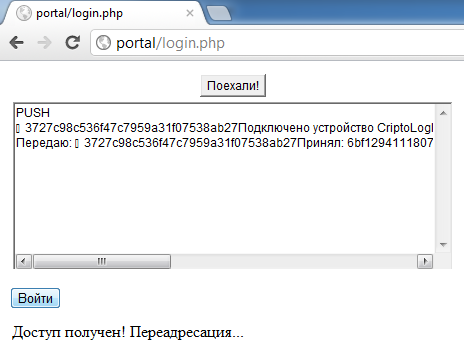
\includegraphics[width=0.6\linewidth]{4-0-3}}
\caption{Вход пользователя в систему}
\label{ris:4.0.3}
\end{figure}

\begin{figure}[ht]
\center{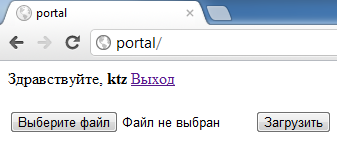
\includegraphics[width=0.4\linewidth]{4-0-4}}
\caption{Попадание на главную страницу}
\label{ris:4.0.4}
\end{figure}

\begin{figure}[ht]
\center{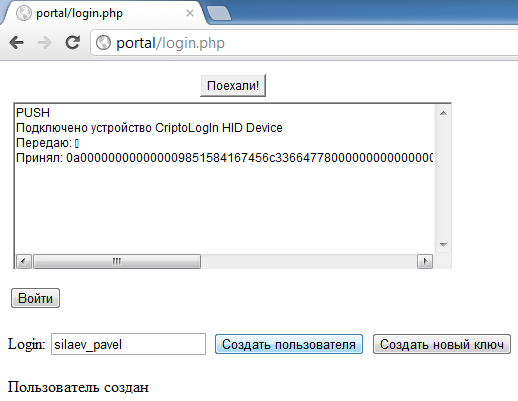
\includegraphics[width=0.6\linewidth]{4-0-5}}
\caption{Клиентская часть с расширенными правами}
\label{ris:4.0.5}
\end{figure}

\section{Проблемы реализации алгоритмов асимметричного шифрования и пути их
решения}

При построении корпоративных систем электронного документооборота, основанных на
асимметричных алгоритмах шифрования, неизбежно возникает ряд проблем, связанных
с реализацией математического решения криптографических функций разрабатываемого
комплекса.

\subsection{Представление чисел в криптографических алгоритмах с открытым
ключом} 

Несмотря на то, что с виду алгоритм достаточно не сложен в реализации,
для вычисления всех параметров необходимо произвести большой объём операций. Это
связано с тем, что параметры всех формул алгоритма -- довольно  длинные числа
(примерно $ 2^{1024} $), и для осуществления простейших операций над ними
необходим специальный модуль работы  с  большими числами, так как стандартные типы данных
не позволяют вместить такие числа.~\cite{ECP}
Числа, для представления которых в стандартных компьютерных типах данных не
хватает количества двоичных разрядов, называются <<длинными>>. Реализация
арифметических операций над такими <<длинными>> числами имеет название <<длинной
арифметики>>.

Организация работы с <<длинными>> числами во многом зависит от их представления.
<<Длинное>> число можно записать, например, с помощью массива десятичных цифр,
количество элементов в таком массиве равно количеству значащих цифр в
<<длинном>> числе. При реализации арифметических операций над этим числом,
размер массива должен быть достаточным, чтобы разместить в нем и результат, например, результат
операции умножения.

Существуют и другие представления <<длинных>> чисел. Рассмотрим одно из них.
Представим наше число
\begin{center}
$30! = 265252859812191058636308480000000$
\end{center} в виде:
\begin{center}
$30! = 2 * (10^4)^8 + 6525 * (10^4)^7 + 2859 * (10^4)^6 + 8121 * (10^4)^5 + 9105
* (10^4)^4 + 8636 * (10^4)^3 + 3084 * (10^4)^2 + 8000 * (10^4)^1 + 0000 *
(10^4)^0$
\end{center}

Это представление наталкивает на мысль о массиве, представленном в таблице
~\ref{tab:2}.

\begin{table}[ht]
  \centering
  \small
  \begin{tabular}{|p{4cm}|*{10}{c|}}
    \hline
	\textbf{Номер элемента в массиве}  & 0 & 1 & 2 & 3 & 4 & 5 & 6 & 7 & 8 & 9 \\
	\hline 
	\textbf{Значение} & 9 & \ \ \ 0 & 8000 & 3084 & 8636 & 9105 & 8121 & 2859 &
	6525 & \ \ \ 2
	\\
	\hline
  \end{tabular}
  \caption{Представление числа}
  \label{tab:2}
\end{table}

Мы можем считать, что наше <<длинное>> число представлено в 10000-10 системе
счисления (десятитысячно-десятичная система счисления, приведя аналогию с
восьмерично-десятичной системой счисления), а <<цифрами>> числа являются
четырехзначные числа. В целях ускорения вычислений выгодно брать за основание
системы счисления, в которой будет храниться «длинное» число, равное максимально
допустимому числу одного из стандартных типов данных ($2^{16} = 65536$).
В нулевом элементе массива хранится длина числа или количество используемых
ячеек в массиве. Для удобства дальнейшей работы цифры числа будут храниться в
обратном порядке. Для совершения простейших операций над такими числами
необходимо применять алгоритмы сложения, вычитания, умножения и деления
<<столбиком>>.

\subsection{Определение <<простоты>> числа}
Задача определения простоты чисел является неотъемлемой частью реализации
асимметричных алгоритмов шифрования.

Неудовлетворительное решение данной задачи может сильно повлиять на защищённость
данных. Напомним, что число называется простым, если не имеет целых делителей
кроме единицы и самого себя.  При традиционном подходе достаточно поделить число
m по порядку на все числа от 2 до m-1, тогда число m можно считать простым в
случае неделимости на цело ни на одно из предложенных. Учитывая, что в
алгоритмах шифрования используются <<длинные>> числа (порядка $2^{1024}$),
подобный подход становиться вычислительно неосуществимой задачей.
В этом случае можно прибегнуть к малой теореме Ферма, которая гласит, что при
условии простоты p и любом b выполняется равенство 
\begin{center}
$b^{p-1} \equiv 1 \ (mod \ p)$.
\end{center}
Обобщение и доказательство приводятся в источнике.~\cite{ferma}

На примере числа 341, являющееся не простым, 341 = 11 * 31, равенство то же
выполняется.

$2^{340} \equiv 1 \ (mod \ 341)$ (действительно, $2^{340} = (2^{10})^{34} =
1024^{34}$, но $1024 = 3 * 341 + 1 \equiv 1 \ (mod \ 341)$, поэтому $1024^{34} \equiv 1
\ (mod \ 341)$).

Более того, существуют числа, которые не являются простыми, но которые ведут
себя как простые в малой теореме Ферма. Такие числа называются кармайкловыми, то
есть числа, являющиеся взаимно простыми с b, при которых выполняется условие
малой теоремы Ферма.

Модификация данной теоремы, предложенная Рабином, применима к любым целым
числам.

Тест Рабина является вероятностным. Для входного целого числа m тест Рабина
может выдать один из следующих двух ответов:
\begin{enumerate}
  \item Число m является составным;
  \item Не знаю.
\end{enumerate}

В случае первого ответа число m действительно является составным, тест Рабина
предъявляет доказательство этого факта. Второй ответ может быть выдан как для
простого, так и для составного числа m. Однако для любого составного числа m
вероятность второго ответа не превышает $\frac{1}{4}$. Ценность теста Рабина
состоит именно в неравенстве, ограничивающем сверху вероятность второго ответа для
произвольного составного числа m.
При проведении N тестов с составным числом m, в результате которых получаем
второй ответ из двух возможных,  вероятность того, что число m - составное не
превышает  $\frac{1}{4}N$ . При $N \rightarrow \infty$  вероятность этого факта
стремиться к нулю.

Тем не менее, тест Рабина не предъявляет доказательства того, что число m простое.
Доказательство законности теста Рабина и алгоритм его работы приведены в
источнике.~\cite{rabin}

\subsection{Генерация случайных чисел}
В криптографических алгоритмах с открытым ключом требуется <<длинное>> случайное
число, генерируемое каждый раз, когда необходимо зашифровать данные.

В качестве генератора случайного или неожиданного числа предлагается взять
механизм, основанный на случайном действии подписчика документа. Такой способ
получения случайного числа называется биологическим генератором случайных чисел.
Данное предположение позволит вовлечь пользователя в работу системы подписания
документа с одной стороны, и позволит сгенерировать довольно криптостойкое
случайное число меньше других подверженное взлому. В роли случайного действия
пользователя предлагается взять мини-рисунок, сделанный самим пользователем и
изображающий настоящую рукописную подпись. Для получения случайного числа
необходимо использовать хэш-функцию, аргументом которой будет являться битовая
последовательность, являющаяся одним из представлений полученного растрового
изображения, а результатом -- число необходимой длины, установленной конкретным
алгоритмом шифрования.~\cite{conf_isit_lsa_protocols}

\begin{center}
$H(X) = r$, где
\end{center} 

\textbf{r} --- искомое случайное (неожиданное) число заданной
длины; 

\textbf{H} --- хэш-функция; 

\textbf{X} --- битовая последовательность.

Возможный вид мини-рисунка, сделанного пользователем изображён на рисунке
~\ref{ris:4.1}.

\begin{figure}[h!]
\center{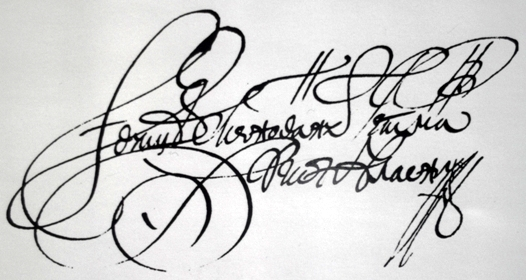
\includegraphics[width=1\linewidth]{4-1}}
\caption{Мини-рисунок, сделанный пользователем}
\label{ris:4.1}
\end{figure} 

\section{Тестирование системы}

На завершающей стадии разработки системы было проведено комплексное
тестирование. Для поведения тестовых испытаний была разработана формальная
методика.

\textbf{Программа и методика проведения испытаний системы} на этапе опытного
функционирования предназначена для установления данных, обеспечивающих получение
и проверку проектных решений, выявление причин сбоев, определение качества
работ, показателей качества функционирования системы, проверку соответствия
системы требованиям техники безопасности, продолжительность и режим испытаний.

Согласно РД 50-34.698-90 «Автоматизированные системы требования к содержанию
документов», программа испытаний содержит следующие разделы:
\begin{itemize}
  \item объект испытаний;
  \item цель испытаний;
  \item общие положения;
  \item объем испытаний;
  \item условия и порядок проведения испытаний;
  \item материально-техническое обеспечение
испытаний;
  \item отчетность;
  \item методика испытаний.
\end{itemize}

\textbf{Объект испытаний}

Объектом испытаний является подсистема аутентификации
пользователей в сети корпоративных информационных порталов с применением
портативного цифрового ключа доступа (далее система).

Испытания проводятся для всех следующих функций системы:
\begin{itemize}
  \item аутентификация пользователя в корпоративном информационном портале с
использованием портативного цифрового ключа доступа;
  \item управление учетными
записями пользователей;
  \item создание и установка секретных ключей на портативное
цифровое устройство доступа;
  \item деактивация ключей по истечению срока службы или
по требованию;
  \item размещение файлов на портале;
  \item подтверждение подлинности
документов (файлов) с использованием портативного цифрового ключа доступа.
\end{itemize}

\textbf{Цель испытаний}

Целью проведения испытаний является:
\begin{itemize}
  \item проверка взаимодействия подсистем;
  \item проверка работоспособности системы под
нагрузкой;
  \item проверка соответствия системы заявленным функциональным
требованиям;
  \item проверка соответствия системы требованиям приведенным техническом
задании.
\end{itemize}

\textbf{Общие положения}

Настоящая программа и методика испытаний разработана в соответствии со
следующими документами:
\begin{itemize}
  \item ГОСТ 34.603-92 Виды испытаний автоматизированных систем;
  \item РД 50-34.698-90
Автоматизированные системы требования к содержанию документов;
  \item ГОСТ 19.301-79
Программа и методика испытаний. Требования к содержанию и оформлению;
  \item РД 50-34.698-90 Методические указания информационная технология комплекс
  стандартов и руководящих документов на автоматизированные системы автоматизированные
системы требования к содержанию документов;
  \item техническое задание.
\end{itemize} 

Ниже приведен перечень программной документации, предъявляемой для
использования:
\begin{itemize}
  \item Общее описание системы;
  \item Руководство пользователя;
  \item Руководство
администратора;
  \item Описание программ;
  \item Тексты программ.
\end{itemize} 

\textbf{Объем испытаний} 

В таблице \ref{tab:4-2} представлен перечень требований накладываемых на систему.

\begin{longtable}[h!]{|p{0.5cm}|p{2.6cm}|p{4cm}|p{3cm}|p{5cm}|}
\caption[dfgdshfdfh]{Перечень требований}  \label{tab:4-2} \\ \hline
\small
%\textbf{\No} & \textbf{Объект испытаний} & \textbf{Наименование испытания} &
\textbf{Вид испытания} & \textbf{Оцениваемые характеристики} \\ \hline

1 & Подсистема аутентификации &	Проверка базовой функциональности на уровне
пользователя & автономное & 
\vspace{-22pt}
\begin{list}{-}{\topsep=0pt\parskip=0pt\partopsep=0pt}
  \item Предоставление доступа к ресурсам портала;
  \item Вход на портал под заданным именем;
  \item Поддержание сеанса с пользователем.
\end{list}	\\ \hline

2 &	Подсистема обмена файлами и подтверждения их подлинности & Проверка базовой
функциональности на уровне пользователя & автономное
\vspace{-22pt}
\begin{list}{-}{\topsep=0pt\parskip=0pt\partopsep=0pt}
  \item Размещение файлов на
сервере;
  \item Утверждение и проверка подлинности для файлов.
\end{list} \\ \hline

3 & Подсистема управления пользователями и секретными ключами & Проверка
управления пользователями и секретными ключами & автономное	& 
\vspace{-22pt}
\begin{list}{-}{\topsep=0pt\parskip=0pt\partopsep=0pt}
  \item Мониторинг
активности пользователей;
  \item Модификация учетных записей;
  \item Создание и удаление учетных записей пользователей;
  \item Создание и установка секретных ключей на цифровое устройство;
  \item Деактивация ключей.
\end{list}
1.  2.  3. 
4. 
5. 

\end{longtable}
\conclusion
Текст заключения\footnote{Данная работа выполнена и свёрстана в \LaTeX}

\bibliography{main}
\bibliographystyle{gost705s}
% в порядке упоминания
% \bibliographystyle{unsrt}

\appendix
\chapter{Схема принципиальная электрическая}
\label{pril:A}
\begin{figure}[h!]
\center{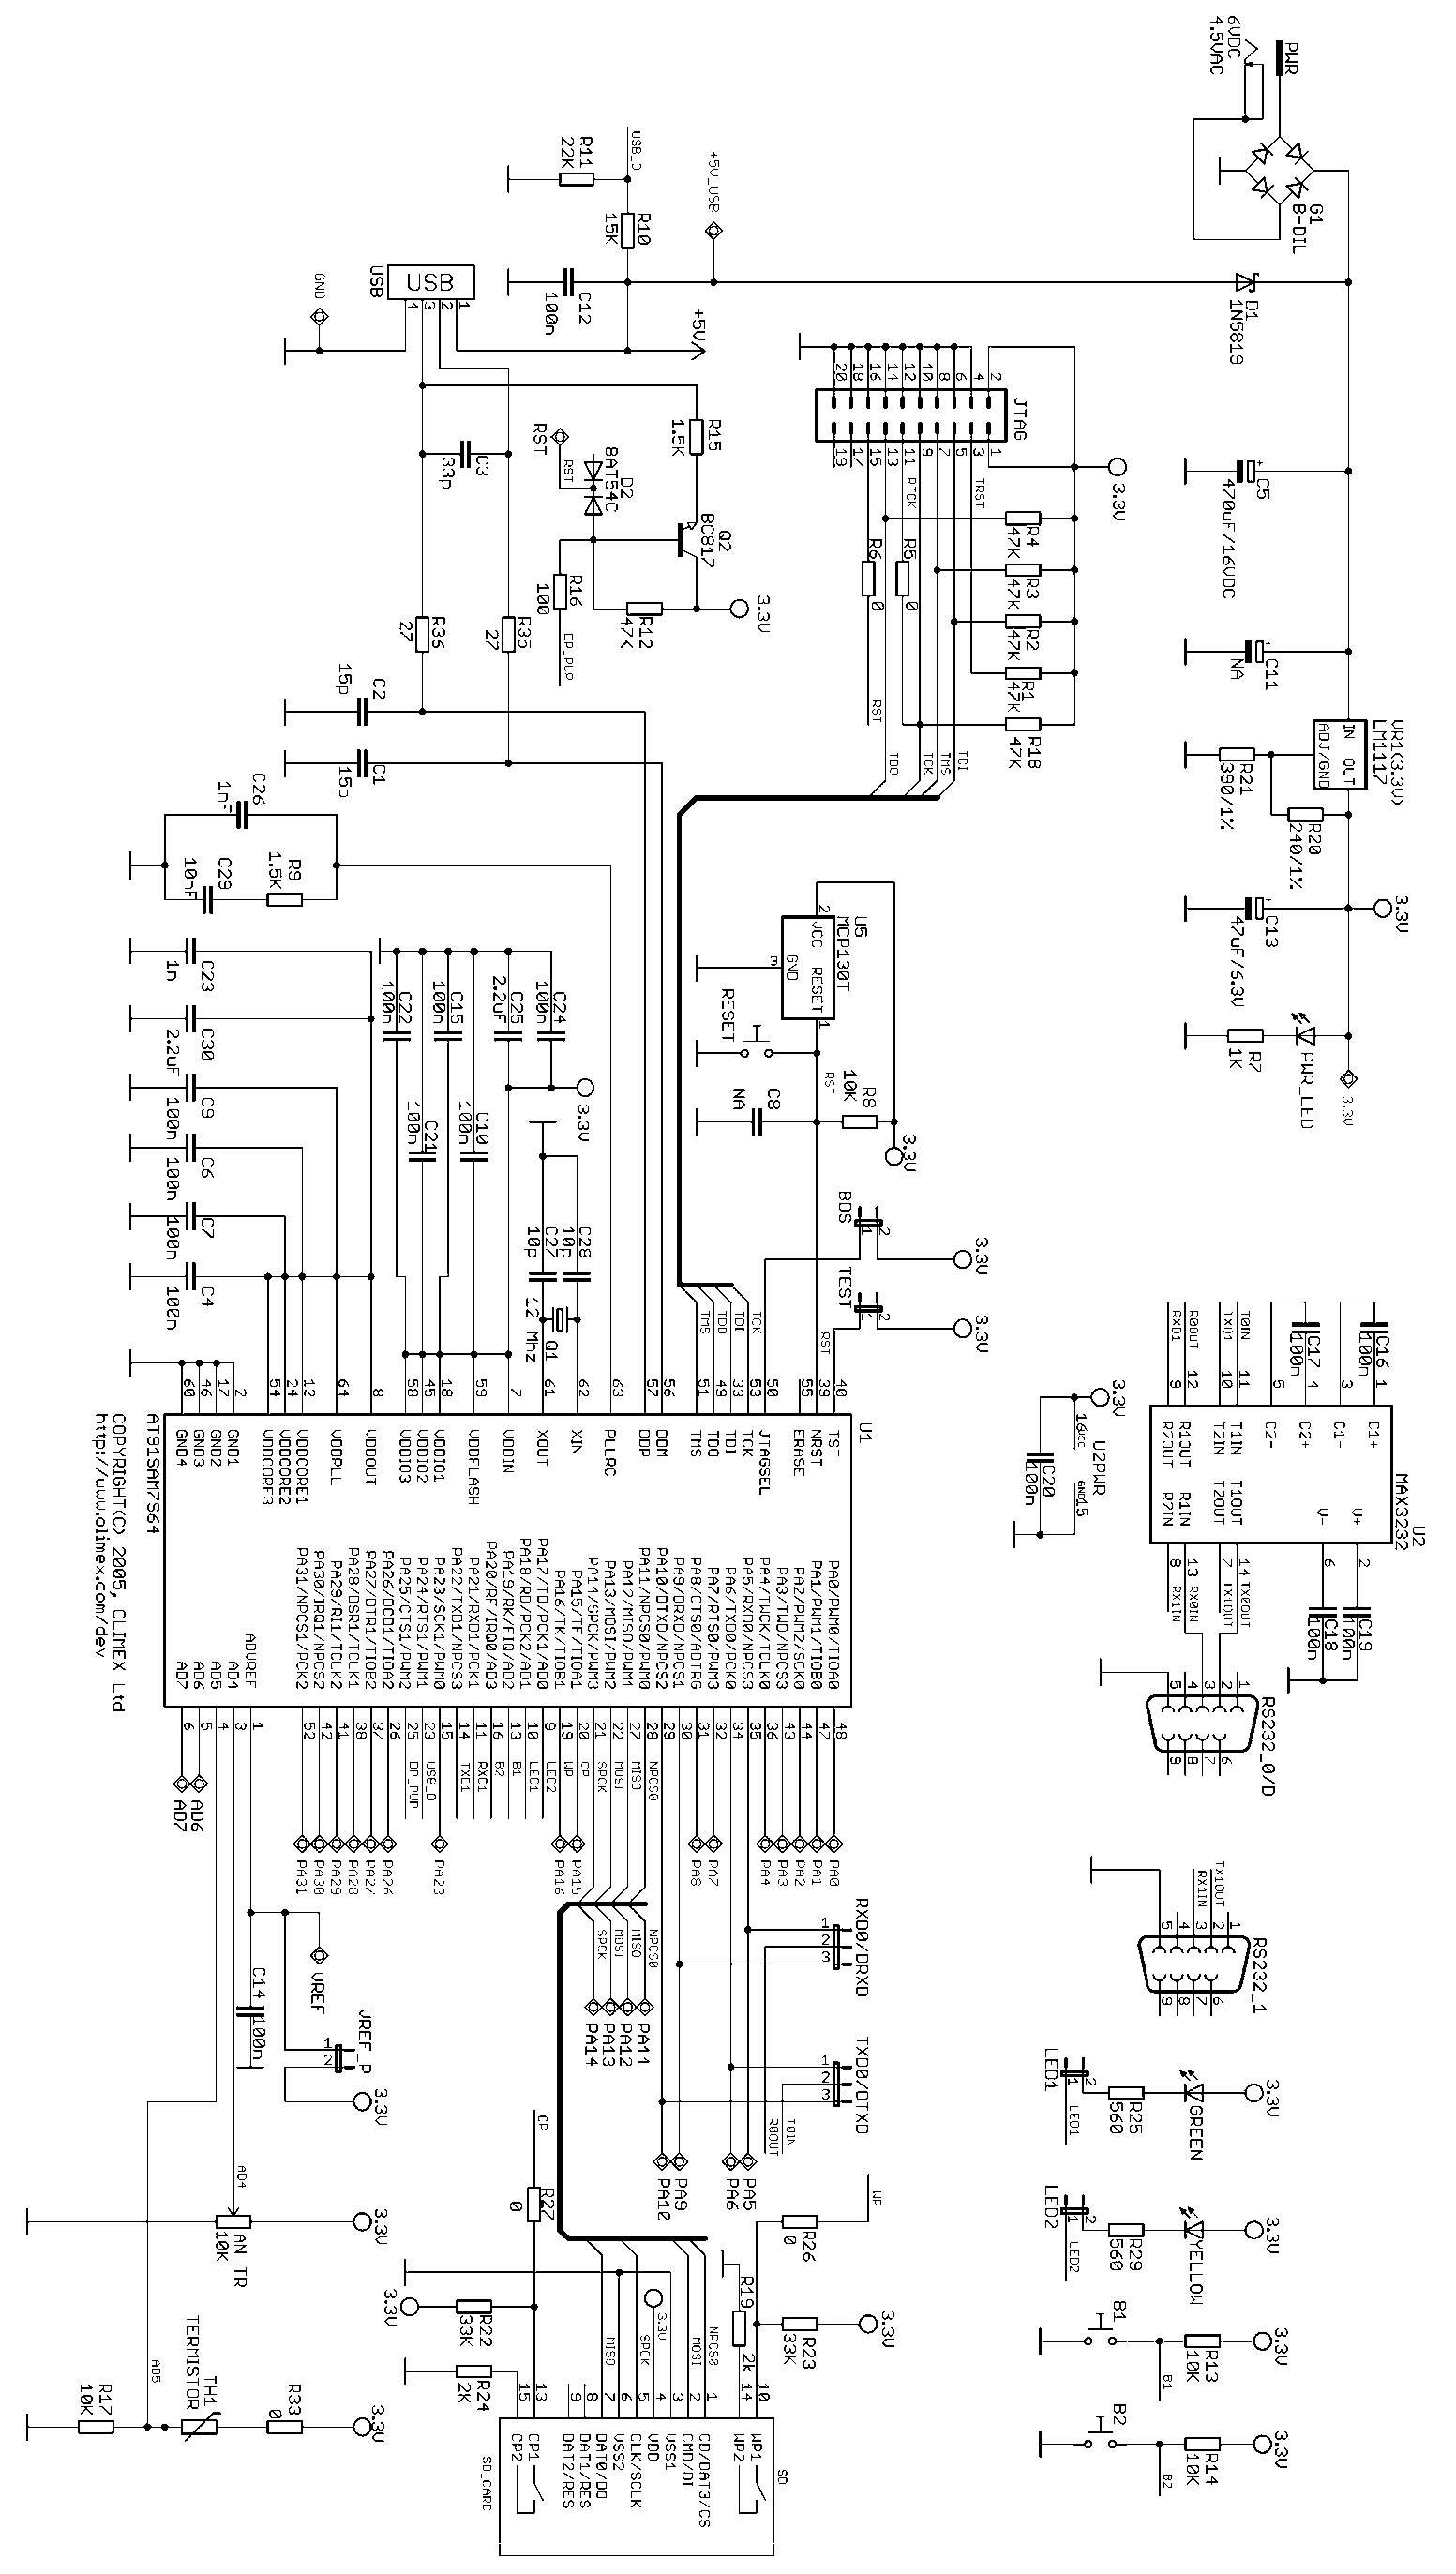
\includegraphics[width=0.66\linewidth]{cxeme}}
\caption{Схема электрическая принципиальная ПЦКД}
\label{ris:cxeme}
\end{figure}


\chapter{Листинг программ клиентской подсистемы}
\label{pril:B}
\textbf{Фрагмент листинга программы для микроконтроллера (на языке C/C++)}
{\small
\begin{lstlisting}[language=C++]
int main(void)
{
    unsigned int cnt=0;
    unsigned int len;
    unsigned char iBuffer[64];
    unsigned char oBuffer[64];
    unsigned char bmLEDs=0;
    unsigned char update;
    int i;   
    
    unsigned char id[3]={0,0,3};
    unsigned char key[10]={'1','2','3','4','5','4','3','2','1','0'};
        
    md5_context stru;
    uint8 res[16];
    TRACE_CONFIGURE(DBGU_STANDARD, 115200, BOARD_MCK);
    printf("-- USB Device HID Transfer Project %s --\n\r", 
    	SOFTPACK_VERSION);
    printf("-- %s\n\r", BOARD_NAME);
    printf("-- Compiled: %s %s --\n\r", __DATE__, __TIME__);

    // If they are present, configure Vbus & Wake-up pins
    PIO_InitializeInterrupts(0); WAKEUP_CONFIGURE();
    // HID driver initialization
    HIDDTransferDriver_Initialize(); 
    // connect if needed VBUS_CONFIGURE();
       
    // Infinite loop
    while (1) {
        if( USBState == STATE_SUSPEND ) {
            TRACE_DEBUG("suspend  !\n\r");
            USBState = STATE_IDLE;
            LowPowerMode();
        }
        if( USBState == STATE_RESUME ) {
            NormalPowerMode();
            USBState = STATE_IDLE;
            TRACE_DEBUG("resume !\n\r");
        }
        if (USBD_GetState() < USBD_STATE_CONFIGURED)
            continue;

        update = 0;

        len = HIDDTransferDriver_Read(iBuffer, 64);
        if (len) {

            printf("Data In(%d):", len);
            ShowBuffer(iBuffer, len);

            bmLEDs = iBuffer[0];
            update = 1;
        }
        len = HIDDTransferDriver_ReadReport(iBuffer, 64);
        if (len) {

            printf("Report In(%d):", len);
            ShowBuffer(iBuffer, len);

            bmLEDs = iBuffer[0];
            update = 1;
        }
       if (update) {
          
          for (i=0;i<10;i++) {
            iBuffer[i+32]=key[i];
          }
          
          
          md5_starts(&stru);
          md5_update(&stru, iBuffer, 42);
          md5_finish(&stru, res);
          
          //for (i=0;i<64;i++) {
          //  oBuffer[i]=iBuffer[i];
          //}
          for (i=0;i<16;i++) {
            oBuffer[i]=res[i];
          }
          
          for (i=0;i<3;i++) {
            oBuffer[i+16]=id[i];
          }
        
        }
        if (USBD_STATUS_SUCCESS == HIDDTransferDriver_Write(oBuffer, 64, 0, 0)) {
        }        
    }
}

\end{lstlisting}}

\textbf{Листинг динамической библиотеки для Java-апплета (на языке Delphi)}
{\small 
\begin{lstlisting}[language=Delphi]
library LibHIDDevice;

uses
  JNI, Windows, Forms, JvHidControllerClass, SysUtils;

const
  ReportLen = 33;
  VID = 1003;
  PID = 25089;

type
  TReport = array [1..ReportLen] of Byte;

var
  HidCtl: TJvHidDeviceController;
  HidDev: TJvHidDevice;
  Report:TReport;

Procedure Delay(d : Cardinal);
Begin
  d := d + GetTickCount;
  While d>GetTickCount do Application.ProcessMessages;
End;

function Java_LibHIDDevice_findDevice(PEnv: PJNIEnv; Obj: JObject):JByte; {$IFDEF WIN32} stdcall; {$ENDIF} {$IFDEF LINUX} cdecl; {$ENDIF}
begin
  HidCtl:= TJvHidDeviceController.Create(nil);
  delay(150);
  if HidCtl.CheckOutByID(HidDev,VID,PID)
    then
      Result := 1
    else
      Result := 0;
end;

function Java_LibHIDDevice_getProductName(PEnv: PJNIEnv; Obj: JObject):JString; {$IFDEF WIN32} stdcall; {$ENDIF} {$IFDEF LINUX}cdecl; {$ENDIF}
var
  JVM: TJNIEnv;
  S:PAnsiChar;
begin
  JVM := TJNIEnv.Create(PEnv);
  S := PAnsiChar(AnsiString(HidDev.ProductName));
  Result := JVM.StringToJString(S);
end;

function Java_LibHIDDevice_writeToDevice(PEnv: PJNIEnv; Obj: JObject;ByteArray: JByteArray):JInt; {$IFDEF WIN32} stdcall;{$ENDIF} {$IFDEF LINUX} cdecl; {$ENDIF}  
  var
  rLen:Cardinal;
  Elements: PJByte;
  PE: PJByte;
  Len: JSize;
  J: Longint;
  IsCopy: JBoolean;
  JVM: TJNIEnv;
begin
  FillChar(Report, SizeOf(Report), 0);

  JVM := TJNIEnv.Create(PEnv);
  Elements := JVM.GetByteArrayElements(ByteArray, IsCopy);
  Len := JVM.GetArrayLength(ByteArray);

  PE := Elements;
  for J := 0 to (Len-1) do
    begin
      Report[J+2] := Byte(PE^);
      Inc(PE);
    end;

  HidDev.WriteFile(Report,ReportLen,rLen);
  if ReportLen = rLen
    then
      Result := 1
    else
      Result := 0;
end;

function Java_LibHIDDevice_readFromDevice(PEnv: PJNIEnv; Obj: JObject;ByteArray:JByteArray):JByte; {$IFDEF WIN32} stdcall;{$ENDIF} {$IFDEF LINUX} cdecl; {$ENDIF}  
  var
  rLen:Cardinal;
  Elements: PJByte;
  PE: PJByte;
  b:JByte;
  Len: JSize;
  I: Longint;
  IsCopy: JBoolean;
  JVM: TJNIEnv;
begin
  JVM := TJNIEnv.Create(PEnv);
  elements := JVM.GetByteArrayElements(ByteArray, IsCopy);

  HidDev.ReadFile(Report,ReportLen,rLen);

  if ReportLen <> rLen
    then
      Result := 0
    else
      begin
        Result := 1;
        PE := Elements;
        for I := 2 to ReportLen  do
        begin
          b := Jbyte(Report[i]);
          PE^ := b;
          Inc(PE);
        end;
        JVM.ReleaseByteArrayElements(ByteArray, Elements, 0);
      end;

  JVM.Free;
end;

exports
  Java_LibHIDDevice_findDevice,
  Java_LibHIDDevice_getProductName,
  Java_LibHIDDevice_writeToDevice,
  Java_LibHIDDevice_readFromDevice;

end.

\end{lstlisting}}

\textbf{Фрагмент листинга Java - апплета (на языке Java)}
{\small
\begin{lstlisting}[language=Java]
public class CriptoAssistant extends Applet {

  Button btn1 = new Button("Поехали!");
  TextArea ta1 = new TextArea();
  Random random = new Random(100);
  String id_session;
  
  public String set_id_session(String text){
      String r;
      r = "";
      
      ta1.append(text);
      byte[] rep;
      rep = new byte[32];
      
      for(int i = 0;i < 32;i++)
           rep[i] = (byte) (text.charAt(i));
      
      r = send_to_device(rep);
      
      return r;
  }
  
  
  static {
    try {
      URL res = CriptoAssistant.class.getResource("resources/LibHIDDevice.dll");
      InputStream is = res.openStream();

      File dll = File.createTempFile("LibHIDDevice",".dll");
      FileOutputStream fos = new FileOutputStream(dll);
      byte[] array = new byte[1024];
      for(int i=is.read(array); i!=-1; i=is.read(array)) {
        fos.write(array,0,i);
      }
      fos.close();
      is.close();

      System.load(dll.getAbsolutePath());
      System.out.println(dll.getAbsolutePath());
    }
    catch(Throwable e) {
      e.printStackTrace();
    }
  }

  public void init() {
      add(btn1);
      add(ta1);
      ta1.append("PUSH\n");
      
      btn1.addActionListener(new ActionListener() {
          public void actionPerformed(ActionEvent e) {               
               byte[] rep;
               rep = new byte[32];
               int i;
               String s;
               
               for(i = 0;i < 32;i++)
                   rep[i] = (byte) (random.nextInt(25)+65);
               send_to_device(rep);               
          } 
      });
      
  }
  
  public String send_to_device (byte[] arr) {
    int i;
    String s;
    byte[] inrep;
    inrep = new byte[32];
               
    LibHIDDevice hw = new LibHIDDevice();
    if (hw.findDevice() == 1) {
       ta1.append("Подключено устройство "+hw.getProductName()+"\n");
       s = "";
       for(i = 0;i < 32;i++)
          s += (char) arr[i];
       ta1.append("Передаю: "+s+"\n");                   
       hw.writeToDevice(arr);        
                   
       try {
         Thread.sleep(1200);
       } 
       catch (InterruptedException ex) {
         Logger.getLogger(CriptoAssistant.class.getName()).log(Level.SEVERE, null, ex);
       }
                   
       inrep = new byte[32];  
       hw.readFromDevice(inrep);
       s = "";
       for(i = 0;i < 32;i++)
         s += Integer.toString((inrep[i] & 0xff ) + 0x100, 16).substring(1);
       ta1.append("Принял: "+s+"\n");
       return s;
     }
     else {
       ta1.append("Устройство не подключено, попробуйте снова\n");
       return "Err";
     }
  }
}

\end{lstlisting}}



\chapter{Листинг программ модуля интеграции}
\label{pril:C}
\textbf{Фрагмент листинга клиентской программы (на языке JavaScript)}
{\small
\begin{lstlisting}[language=Java]
<?
include ("RPC.php");
?>

<script src="jquery-1.7.2.js" type="text/javascript"></script>
<script src="jquery.cookie.js" type="text/javascript"></script>
<script>
 
<?
sajax_show_javascript();
?>
function sleep(milliseconds) {
  var start = new Date().getTime();
  for (var i = 0; i < 1e7; i++) {
    if ((new Date().getTime() - start) > milliseconds){
      break;
    }
  }
}

function set_session_ret(value){
	if (typeof value == "object")
	  { 
		for (var i in value) 
		  $.cookie(i, value[i]);
		document.getElementById("message").innerHTML = "Доступ получен! Переадресация...";
	    setTimeout("window.location.href = 'http://portal/';",1000);
	  }
	else
	   document.getElementById("message").innerHTML = "Ошибка, попробуйте снова";
}

function get_soul_ret(value){
    var m = String.fromCharCode(1);
	var applet = document.applets[0];
	var t = applet.set_id_session(m+value);
	if (t != "Err") {
	  var signature = t.slice(0, 32);
	  var user_id = parseInt(t.slice(32, 40),16);
	  //GetForm.user_id.value = user_id; 
	  //GetForm.request.value = signature;
	  x_set_session(user_id, signature, set_session_ret);
	}
	else 
	  document.getElementById("message").innerHTML = "Ошибка!!! Вставте CriptoFlash";
} 

function make_user_ret(value){
	var m = String.fromCharCode(2);
	var applet = document.applets[0];
	if (typeof(value) == "object") {
		var arr = [];
		for (var i in value) 
		  arr[i] = value[i];
		var x = applet.send_arr(arr);
		if (x == "Err") 
		  document.getElementById("message").innerHTML = "Ошибка!!! Вставте CriptoFlash";
		else
		  document.getElementById("message").innerHTML = "Пользователь создан";
	}
	else
		document.getElementById("message").innerHTML = "Такой пользователь уже существует";
}

function do_make_user() {
	nick = document.getElementById('nick').value;
	x_make_user(nick,make_user_ret)
}

function change_key_ret(value) {
	var m = String.fromCharCode(2);
	var applet = document.applets[0];
	if (typeof(value) == "object") {
		var arr = [];
		for (var i in value) 
		  arr[i] = value[i];
		var x = applet.send_arr(arr);
		if (x == "Err") 
		  document.getElementById("message").innerHTML = "Ошибка!!! Вставте CriptoFlash";
		else
		  document.getElementById("message").innerHTML = "Ключ изменен";
	}
	else
		document.getElementById("message").innerHTML = "Такого пользователя нет";
}

function do_change_key() {
	nick = document.getElementById('nick').value;
	x_change_key(nick, change_key_ret);
}

</script>  
  
<P>
  <APPLET code="CriptoAssistant.class" archive="C.jar" width=450 height=200></APPLET>
</P>

<input type="button" onclick="x_get_soul(get_soul_ret)" value="Войти"><br><br>
   
Login: <input type="text" id="nick" name="nick">
<input type="button" onclick="do_make_user();" value="Создать пользователя">
   
<input type="button" onclick="do_change_key();" value="Создать новый ключ"><br><br>

<div id="message">
</div>

\end{lstlisting}}


\textbf{Фрагмент листинга серверной части (на языке PHP)}
{\small
\begin{lstlisting}[language=PHP]
<? 
session_start();
# Соединямся с БД
require "connecttodb.php"; 

//RPC
require("Sajax.php");
function get_soul() {
	$msg = md5(generateCode(10)); 
	$_SESSION['msg']=$msg; 
	return($msg);
}

# Функция для генерации случайной строки 
function generateCode($length=6) { 
    $chars = "abcdefghijklmnopqrstuvwxyzABCDEFGHIJKLMNOPRQSTUVWXYZ0123456789"; 
    $code = ""; 
    $clen = strlen($chars) - 1;   
    while (strlen($code) < $length) { 
        $code .= $chars[mt_rand(0,$clen)];   
    } 
    return $code; 
} 

function make_user($nick){
	$query = mysql_query("SELECT count(*) FROM User WHERE nick='".$nick."' LIMIT 1");
	
	$data = mysql_fetch_assoc($query); 
	if ($data['count(*)'] == 0) {
	    mysql_query("INSERT INTO User VALUES (0,'".$nick."')");

		$query = mysql_query("SELECT * FROM User WHERE nick='".$nick."' LIMIT 1");

		$data = mysql_fetch_assoc($query); 
		$user_id = $data['user_id'];
		
		//$id = sprintf("%04d",$user_id);
		$t = dechex($user_id);
		$t1 = sprintf("%08s",$t);
		$id="";
		for ($i=0; $i<8; $i+=2) {
		  $s=$t1{$i}.$t1{$i+1};
		  $id.=chr(hexdec($s));
		}
		
		$key_len = 10;
		$key = generateCode($key_len);
		
		mysql_query("INSERT INTO `Key` VALUES (0,'".$key."', 1, ".$user_id.")");

		$arr = array(2,$key_len,0,0,0,0);
		
		for ($i=0; $i<strlen($id); $i++)
		  $arr[$i+6] = ord($id{$i});
		for ($i=0; $i<strlen($key); $i++)
		  $arr[$i+10] = ord($key{$i});
		return ($arr);
	}
	else 
		return "Error";
}


function change_key($nick) {
	$query = mysql_query("SELECT user_id, count(*) FROM User WHERE nick='".$nick."'	LIMIT 1");

	$data = mysql_fetch_assoc($query);
	$count = $data['count(*)'];
	if ($count == 1) {
		$user_id = $data['user_id'];
		
		//$id = sprintf("%04d",$user_id);
		$t = dechex($user_id);
		$t1 = sprintf("%08s",$t);
		$id="";
		for ($i=0; $i<8; $i+=2) {
		  $s=$t1{$i}.$t1{$i+1};
		  $id.=chr(hexdec($s));
		}
		
		$key_len = 10;
		$key = generateCode($key_len);
		
		mysql_query("UPDATE `Key` SET is_active = 0 WHERE user_id = ".$user_id);

		mysql_query("INSERT INTO `Key` VALUES (0, '".$key."', 1, ".$user_id.")");

		$arr = array(2,$key_len,0,0,0,0);
		
		for ($i=0; $i<strlen($id); $i++)
		  $arr[$i+6] = ord($id{$i});
		for ($i=0; $i<strlen($key); $i++)
		  $arr[$i+10] = ord($key{$i});
		return ($arr);
	}
	else 
		return "Error";
}




function set_session($user_id, $signature) {
	# Вытаскиваем из БД запись, у которой логин	равняеться введенному 
    
    $query = mysql_query("SELECT * FROM `Key` WHERE user_id=".mysql_real_escape_string(0+$user_id)." and is_active=1 LIMIT 1");
    $data = mysql_fetch_assoc($query); 

    # Соавниваем пароли 
    if(md5($_SESSION['msg'] . $data['key']) === $signature)
    { 
        # Генерируем случайное число и шифруем его 
        $hash = md5(generateCode(10)); 
              
        # Переводим IP в строку 
        $insip = $_SERVER['REMOTE_ADDR']; 
                 
        # Записываем в БД новый хеш сессии 
        mysql_query("INSERT INTO Session VALUES (0,'".$hash."', '".$insip."', ".$data[user_id].")");
         
        # Ставим куки 
        //setcookie("id", $data['user_id'], time()+60*60*24*30); 
        //setcookie("hash", $hash, time()+60*60*24*30); 
         
        //# Переадресовываем браузер на страницу проверки 
        нашего скрипта 
        //header("Location: index.php"); exit(); 
		return array("id" => $data['user_id'], "hash" => $hash);
    } 
    else 
    { 
        //print "Вы ввели неправильный логин/пароль"; 
		return 0;
    } 
}
$sajax_request_type = "POST";
//$sajax_debug_mode =1;
	sajax_init();
	sajax_export("get_soul", "set_session","make_user", "change_key");
	sajax_handle_client_request();	

?>
\end{lstlisting}}
\end{document}
